\documentclass[11pt]{article}
\usepackage{fullpage}
\usepackage{float}
\usepackage{graphicx}
\usepackage{amssymb}
\usepackage{subcaption}
\usepackage{mwe}
\usepackage{epstopdf}
\usepackage{color,verbatim}
\usepackage{pgfplots}
\usepackage{bm}
\usepackage{listings}
\usepackage{mathtools}          %loads amsmath as well
\usepackage{titling}
\DeclareGraphicsRule{.tif}{png}{.png}{`convert #1 `dirname #1`/`basename #1 .tif`.png}
%\usepackage{doublespace}

\begin{document}
\title{Weekly Status Report}
\author{Development of a 1D Adaptive Wavelet Collocation Code \\
Brandon Gusto \\}
\date{Week Beginning 8/28/2017}

\maketitle
%
\section{Summary of method}
The adaptive wavelet collocation method for differential equations has a number of merits which may make it a viable
alternative to traditional finite element, finite volume, or high order finite difference methods for certain problems. 
Some important advantages include the following:
\begin{itemize}
    \item the multiresolution properties of wavelets allow for natural grid adaptation
    \item the existence of a fast $\mathcal{O}(\mathcal{N})$ scheme for computation of wavelet coefficients and 
          spatial derivatives
    \item the ability of second-generation wavelets to adapt to complex geometries
\end{itemize}
\subsection{Dyadic Grid}
The method makes use of a dyadic grid. Each grid level is defined by 
\begin{equation}
    \mathcal{G}^j= \{ x_{k}^{j} \in \Omega : k \in \mathcal{K}^j \}, j \in \mathcal{Z},
\end{equation}
where $\mathcal{K}^j$ is the integer set representing the spatial locations in the grid at level $j$. The grids are 
nested, implying that $\mathcal{G}^{j} \subset \mathcal{G}^{j+1}$. In other words, the points at level $x^{j}$ are 
a perfect subset of the points at level $x^{j+1}$. This can also be demonstrated by the relation that 
$x_{k}^{j}=x_{2k}^{j+1}$.
\subsection{Interpolating Subdivision}
The interpolating subdivision scheme is central to the second-generation wavelet collocation approach. The scheme is used to
approximate values at odd points $x_{2k+1}^{j+1}$ by constructing interpolating polynomials of order $2N-1$ with the points
at grid level $j$. Lagrange polynomials are used, and the method can be used with a uniform grid or with 
nonuniform points such as Chebychev points. The interpolating scheme is 
\begin{equation}
    f^j(x_{2k+1}^{j+1})=\sum_{l=-N+1}^{N} w_{k,l}^{j} f(x_{k+l}^{j}),
\end{equation}
where the coefficients $w_{k,l}^{j}$ are the lagrange polynomials $L_{2N,k+l}(x)$ evaluated at $x=x_{2k+1}^{j+1}$. The 
lagrange polynomial in this notation is given by 
\begin{equation}
    L_{2N,k+l}(x)=\prod_{ \substack{ i=k-(N+1) \\ i\neq k+l } }^{k+2N} \frac{x-x_i}{x_{k+l}-x_i}
\end{equation}
For a uniform grid, the coefficients should be constant irrespective of the grid level $j$.
\subsection{Fast Wavelet Transform}
The existence of a fast wavelet transform is one of the more attractive qualities of the method. The transform makes use of the 
interpolating subdivision algorithm for the calculation of the scaling and detail wavelet coefficients. The forward wavelet transform is given by
\begin{equation}
	\begin{split}
		d_{k}^{j} &= \frac{1}{2} \left( c_{2k+1}^{j+1}-\sum_{l} w_{k,l}^{j} c_{2k+2l}^{j+1} \right), \\
		c_{k}^{j} &= c_{2k}^{j+1},
	\end{split}
\end{equation}
and the inverse transform is given by 
\begin{equation}
	\begin{split}
		c_{2k+1}^{j+1} &= 2 d_{k}^{j}  + \sum_{l} w_{k,l}^{j} c_{k+l}^{j}, \\
		c_{2k}^{j+1} &= c_{k}^{j}.
	\end{split}
\end{equation}
Note that this second-generation wavelet transform does not include the lifting scheme. When using the lifting scheme,
polynomials are also constructed from odd to even points.
\subsection{Wavelet Construction}
The construction of second-generation wavelets makes use of the dyadic grid. The interpolating subdivision scheme is 
used to interpolate functional values defined at points on level $j$, to odd points (i.e. $x_{2k+1}^{j+1}$) at the next
higher level of resolution. This scheme is used to construct the scaling and detail wavelet functions. Examples of the scaling and detail functions are shown in Figure 1 and Figure 2 respectively.
The computation of the wavelet functions is done using the inverse wavelet transform. To obtain the scaling function $\phi_{m}^{j}(x)$, from (5) set $c_{k}^{j}=\delta_{k,m}, \forall k \in \mathcal{K}^j$, where $\delta_{k,m}$ is the Kronecker delta function defined by
\[ \delta_{k,m} = \begin{cases} 
      1 & k=m \\
      0 & k \neq m.
   \end{cases}
\]
Then let all $d_{l}^{j'}=0, \forall l \in \mathcal{L}^{j'}$ and perform the inverse transform up to an arbitrarily high level of resolution $J$. The wavelet $\psi_{l}^{j}$ is computed by setting $d_{m}^{j'} = \delta_{j',j} \delta_{l,m}, \forall l \in \mathcal{L}^{j}, \forall j \geq j$, and also $c_{k}^{j}, \forall k \in \mathcal{K}^j$. Then perform the inverse wavelet transform up to an arbitrarily high level of resolution $J$.
\begin{figure}
	\center
	% GNUPLOT: LaTeX picture
\setlength{\unitlength}{0.240900pt}
\ifx\plotpoint\undefined\newsavebox{\plotpoint}\fi
\sbox{\plotpoint}{\rule[-0.200pt]{0.400pt}{0.400pt}}%
\begin{picture}(1500,900)(0,0)
\sbox{\plotpoint}{\rule[-0.200pt]{0.400pt}{0.400pt}}%
\put(171.0,131.0){\rule[-0.200pt]{4.818pt}{0.400pt}}
\put(151,131){\makebox(0,0)[r]{$-0.2$}}
\put(1419.0,131.0){\rule[-0.200pt]{4.818pt}{0.400pt}}
\put(171.0,252.0){\rule[-0.200pt]{4.818pt}{0.400pt}}
\put(151,252){\makebox(0,0)[r]{$0$}}
\put(1419.0,252.0){\rule[-0.200pt]{4.818pt}{0.400pt}}
\put(171.0,374.0){\rule[-0.200pt]{4.818pt}{0.400pt}}
\put(151,374){\makebox(0,0)[r]{$0.2$}}
\put(1419.0,374.0){\rule[-0.200pt]{4.818pt}{0.400pt}}
\put(171.0,495.0){\rule[-0.200pt]{4.818pt}{0.400pt}}
\put(151,495){\makebox(0,0)[r]{$0.4$}}
\put(1419.0,495.0){\rule[-0.200pt]{4.818pt}{0.400pt}}
\put(171.0,616.0){\rule[-0.200pt]{4.818pt}{0.400pt}}
\put(151,616){\makebox(0,0)[r]{$0.6$}}
\put(1419.0,616.0){\rule[-0.200pt]{4.818pt}{0.400pt}}
\put(171.0,738.0){\rule[-0.200pt]{4.818pt}{0.400pt}}
\put(151,738){\makebox(0,0)[r]{$0.8$}}
\put(1419.0,738.0){\rule[-0.200pt]{4.818pt}{0.400pt}}
\put(171.0,859.0){\rule[-0.200pt]{4.818pt}{0.400pt}}
\put(151,859){\makebox(0,0)[r]{$1$}}
\put(1419.0,859.0){\rule[-0.200pt]{4.818pt}{0.400pt}}
\put(171.0,131.0){\rule[-0.200pt]{0.400pt}{4.818pt}}
\put(171,90){\makebox(0,0){$-4$}}
\put(171.0,839.0){\rule[-0.200pt]{0.400pt}{4.818pt}}
\put(330.0,131.0){\rule[-0.200pt]{0.400pt}{4.818pt}}
\put(330,90){\makebox(0,0){$-3$}}
\put(330.0,839.0){\rule[-0.200pt]{0.400pt}{4.818pt}}
\put(488.0,131.0){\rule[-0.200pt]{0.400pt}{4.818pt}}
\put(488,90){\makebox(0,0){$-2$}}
\put(488.0,839.0){\rule[-0.200pt]{0.400pt}{4.818pt}}
\put(647.0,131.0){\rule[-0.200pt]{0.400pt}{4.818pt}}
\put(647,90){\makebox(0,0){$-1$}}
\put(647.0,839.0){\rule[-0.200pt]{0.400pt}{4.818pt}}
\put(805.0,131.0){\rule[-0.200pt]{0.400pt}{4.818pt}}
\put(805,90){\makebox(0,0){$0$}}
\put(805.0,839.0){\rule[-0.200pt]{0.400pt}{4.818pt}}
\put(964.0,131.0){\rule[-0.200pt]{0.400pt}{4.818pt}}
\put(964,90){\makebox(0,0){$1$}}
\put(964.0,839.0){\rule[-0.200pt]{0.400pt}{4.818pt}}
\put(1122.0,131.0){\rule[-0.200pt]{0.400pt}{4.818pt}}
\put(1122,90){\makebox(0,0){$2$}}
\put(1122.0,839.0){\rule[-0.200pt]{0.400pt}{4.818pt}}
\put(1281.0,131.0){\rule[-0.200pt]{0.400pt}{4.818pt}}
\put(1281,90){\makebox(0,0){$3$}}
\put(1281.0,839.0){\rule[-0.200pt]{0.400pt}{4.818pt}}
\put(1439.0,131.0){\rule[-0.200pt]{0.400pt}{4.818pt}}
\put(1439,90){\makebox(0,0){$4$}}
\put(1439.0,839.0){\rule[-0.200pt]{0.400pt}{4.818pt}}
\put(171.0,131.0){\rule[-0.200pt]{0.400pt}{175.375pt}}
\put(171.0,131.0){\rule[-0.200pt]{305.461pt}{0.400pt}}
\put(1439.0,131.0){\rule[-0.200pt]{0.400pt}{175.375pt}}
\put(171.0,859.0){\rule[-0.200pt]{305.461pt}{0.400pt}}
\put(30,495){\makebox(0,0){$\phi(x)$}}
\put(805,29){\makebox(0,0){$x$}}
\put(171,252){\usebox{\plotpoint}}
\put(567,251.67){\rule{1.204pt}{0.400pt}}
\multiput(567.00,251.17)(2.500,1.000){2}{\rule{0.602pt}{0.400pt}}
\put(572,252.67){\rule{1.204pt}{0.400pt}}
\multiput(572.00,252.17)(2.500,1.000){2}{\rule{0.602pt}{0.400pt}}
\put(577,253.67){\rule{1.204pt}{0.400pt}}
\multiput(577.00,253.17)(2.500,1.000){2}{\rule{0.602pt}{0.400pt}}
\put(582,254.67){\rule{1.204pt}{0.400pt}}
\multiput(582.00,254.17)(2.500,1.000){2}{\rule{0.602pt}{0.400pt}}
\put(587,255.67){\rule{1.204pt}{0.400pt}}
\multiput(587.00,255.17)(2.500,1.000){2}{\rule{0.602pt}{0.400pt}}
\put(592,256.67){\rule{1.204pt}{0.400pt}}
\multiput(592.00,256.17)(2.500,1.000){2}{\rule{0.602pt}{0.400pt}}
\put(171.0,252.0){\rule[-0.200pt]{95.396pt}{0.400pt}}
\put(602,257.67){\rule{1.204pt}{0.400pt}}
\multiput(602.00,257.17)(2.500,1.000){2}{\rule{0.602pt}{0.400pt}}
\put(607,259.17){\rule{1.100pt}{0.400pt}}
\multiput(607.00,258.17)(2.717,2.000){2}{\rule{0.550pt}{0.400pt}}
\put(612,260.67){\rule{1.204pt}{0.400pt}}
\multiput(612.00,260.17)(2.500,1.000){2}{\rule{0.602pt}{0.400pt}}
\put(597.0,258.0){\rule[-0.200pt]{1.204pt}{0.400pt}}
\put(632,260.17){\rule{1.100pt}{0.400pt}}
\multiput(632.00,261.17)(2.717,-2.000){2}{\rule{0.550pt}{0.400pt}}
\multiput(637.00,258.95)(0.909,-0.447){3}{\rule{0.767pt}{0.108pt}}
\multiput(637.00,259.17)(3.409,-3.000){2}{\rule{0.383pt}{0.400pt}}
\multiput(642.00,255.93)(0.487,-0.477){7}{\rule{0.500pt}{0.115pt}}
\multiput(642.00,256.17)(3.962,-5.000){2}{\rule{0.250pt}{0.400pt}}
\multiput(647.60,249.09)(0.468,-0.774){5}{\rule{0.113pt}{0.700pt}}
\multiput(646.17,250.55)(4.000,-4.547){2}{\rule{0.400pt}{0.350pt}}
\multiput(651.59,242.93)(0.477,-0.821){7}{\rule{0.115pt}{0.740pt}}
\multiput(650.17,244.46)(5.000,-6.464){2}{\rule{0.400pt}{0.370pt}}
\multiput(656.59,234.93)(0.477,-0.821){7}{\rule{0.115pt}{0.740pt}}
\multiput(655.17,236.46)(5.000,-6.464){2}{\rule{0.400pt}{0.370pt}}
\multiput(661.59,226.60)(0.477,-0.933){7}{\rule{0.115pt}{0.820pt}}
\multiput(660.17,228.30)(5.000,-7.298){2}{\rule{0.400pt}{0.410pt}}
\multiput(666.59,217.93)(0.477,-0.821){7}{\rule{0.115pt}{0.740pt}}
\multiput(665.17,219.46)(5.000,-6.464){2}{\rule{0.400pt}{0.370pt}}
\multiput(671.59,210.26)(0.477,-0.710){7}{\rule{0.115pt}{0.660pt}}
\multiput(670.17,211.63)(5.000,-5.630){2}{\rule{0.400pt}{0.330pt}}
\multiput(676.59,203.26)(0.477,-0.710){7}{\rule{0.115pt}{0.660pt}}
\multiput(675.17,204.63)(5.000,-5.630){2}{\rule{0.400pt}{0.330pt}}
\multiput(681.59,196.59)(0.477,-0.599){7}{\rule{0.115pt}{0.580pt}}
\multiput(680.17,197.80)(5.000,-4.796){2}{\rule{0.400pt}{0.290pt}}
\multiput(686.00,191.94)(0.627,-0.468){5}{\rule{0.600pt}{0.113pt}}
\multiput(686.00,192.17)(3.755,-4.000){2}{\rule{0.300pt}{0.400pt}}
\multiput(691.00,187.95)(0.909,-0.447){3}{\rule{0.767pt}{0.108pt}}
\multiput(691.00,188.17)(3.409,-3.000){2}{\rule{0.383pt}{0.400pt}}
\put(617.0,262.0){\rule[-0.200pt]{3.613pt}{0.400pt}}
\multiput(701.00,186.60)(0.627,0.468){5}{\rule{0.600pt}{0.113pt}}
\multiput(701.00,185.17)(3.755,4.000){2}{\rule{0.300pt}{0.400pt}}
\multiput(706.59,190.00)(0.477,0.821){7}{\rule{0.115pt}{0.740pt}}
\multiput(705.17,190.00)(5.000,6.464){2}{\rule{0.400pt}{0.370pt}}
\multiput(711.59,198.00)(0.477,1.267){7}{\rule{0.115pt}{1.060pt}}
\multiput(710.17,198.00)(5.000,9.800){2}{\rule{0.400pt}{0.530pt}}
\multiput(716.59,210.00)(0.477,1.935){7}{\rule{0.115pt}{1.540pt}}
\multiput(715.17,210.00)(5.000,14.804){2}{\rule{0.400pt}{0.770pt}}
\multiput(721.59,228.00)(0.477,2.602){7}{\rule{0.115pt}{2.020pt}}
\multiput(720.17,228.00)(5.000,19.807){2}{\rule{0.400pt}{1.010pt}}
\multiput(726.59,252.00)(0.477,3.493){7}{\rule{0.115pt}{2.660pt}}
\multiput(725.17,252.00)(5.000,26.479){2}{\rule{0.400pt}{1.330pt}}
\multiput(731.59,284.00)(0.477,4.161){7}{\rule{0.115pt}{3.140pt}}
\multiput(730.17,284.00)(5.000,31.483){2}{\rule{0.400pt}{1.570pt}}
\multiput(736.59,322.00)(0.477,4.718){7}{\rule{0.115pt}{3.540pt}}
\multiput(735.17,322.00)(5.000,35.653){2}{\rule{0.400pt}{1.770pt}}
\multiput(741.59,365.00)(0.477,5.051){7}{\rule{0.115pt}{3.780pt}}
\multiput(740.17,365.00)(5.000,38.154){2}{\rule{0.400pt}{1.890pt}}
\multiput(746.59,411.00)(0.477,5.274){7}{\rule{0.115pt}{3.940pt}}
\multiput(745.17,411.00)(5.000,39.822){2}{\rule{0.400pt}{1.970pt}}
\multiput(751.60,459.00)(0.468,7.207){5}{\rule{0.113pt}{5.100pt}}
\multiput(750.17,459.00)(4.000,39.415){2}{\rule{0.400pt}{2.550pt}}
\multiput(755.59,509.00)(0.477,5.385){7}{\rule{0.115pt}{4.020pt}}
\multiput(754.17,509.00)(5.000,40.656){2}{\rule{0.400pt}{2.010pt}}
\multiput(760.59,558.00)(0.477,5.497){7}{\rule{0.115pt}{4.100pt}}
\multiput(759.17,558.00)(5.000,41.490){2}{\rule{0.400pt}{2.050pt}}
\multiput(765.59,608.00)(0.477,5.274){7}{\rule{0.115pt}{3.940pt}}
\multiput(764.17,608.00)(5.000,39.822){2}{\rule{0.400pt}{1.970pt}}
\multiput(770.59,656.00)(0.477,5.051){7}{\rule{0.115pt}{3.780pt}}
\multiput(769.17,656.00)(5.000,38.154){2}{\rule{0.400pt}{1.890pt}}
\multiput(775.59,702.00)(0.477,4.495){7}{\rule{0.115pt}{3.380pt}}
\multiput(774.17,702.00)(5.000,33.985){2}{\rule{0.400pt}{1.690pt}}
\multiput(780.59,743.00)(0.477,4.161){7}{\rule{0.115pt}{3.140pt}}
\multiput(779.17,743.00)(5.000,31.483){2}{\rule{0.400pt}{1.570pt}}
\multiput(785.59,781.00)(0.477,3.382){7}{\rule{0.115pt}{2.580pt}}
\multiput(784.17,781.00)(5.000,25.645){2}{\rule{0.400pt}{1.290pt}}
\multiput(790.59,812.00)(0.477,2.714){7}{\rule{0.115pt}{2.100pt}}
\multiput(789.17,812.00)(5.000,20.641){2}{\rule{0.400pt}{1.050pt}}
\multiput(795.59,837.00)(0.477,1.712){7}{\rule{0.115pt}{1.380pt}}
\multiput(794.17,837.00)(5.000,13.136){2}{\rule{0.400pt}{0.690pt}}
\multiput(800.59,853.00)(0.477,0.599){7}{\rule{0.115pt}{0.580pt}}
\multiput(799.17,853.00)(5.000,4.796){2}{\rule{0.400pt}{0.290pt}}
\multiput(805.59,856.59)(0.477,-0.599){7}{\rule{0.115pt}{0.580pt}}
\multiput(804.17,857.80)(5.000,-4.796){2}{\rule{0.400pt}{0.290pt}}
\multiput(810.59,847.27)(0.477,-1.712){7}{\rule{0.115pt}{1.380pt}}
\multiput(809.17,850.14)(5.000,-13.136){2}{\rule{0.400pt}{0.690pt}}
\multiput(815.59,828.28)(0.477,-2.714){7}{\rule{0.115pt}{2.100pt}}
\multiput(814.17,832.64)(5.000,-20.641){2}{\rule{0.400pt}{1.050pt}}
\multiput(820.59,801.29)(0.477,-3.382){7}{\rule{0.115pt}{2.580pt}}
\multiput(819.17,806.65)(5.000,-25.645){2}{\rule{0.400pt}{1.290pt}}
\multiput(825.59,767.97)(0.477,-4.161){7}{\rule{0.115pt}{3.140pt}}
\multiput(824.17,774.48)(5.000,-31.483){2}{\rule{0.400pt}{1.570pt}}
\multiput(830.59,728.97)(0.477,-4.495){7}{\rule{0.115pt}{3.380pt}}
\multiput(829.17,735.98)(5.000,-33.985){2}{\rule{0.400pt}{1.690pt}}
\multiput(835.59,686.31)(0.477,-5.051){7}{\rule{0.115pt}{3.780pt}}
\multiput(834.17,694.15)(5.000,-38.154){2}{\rule{0.400pt}{1.890pt}}
\multiput(840.59,639.64)(0.477,-5.274){7}{\rule{0.115pt}{3.940pt}}
\multiput(839.17,647.82)(5.000,-39.822){2}{\rule{0.400pt}{1.970pt}}
\multiput(845.59,590.98)(0.477,-5.497){7}{\rule{0.115pt}{4.100pt}}
\multiput(844.17,599.49)(5.000,-41.490){2}{\rule{0.400pt}{2.050pt}}
\multiput(850.59,541.31)(0.477,-5.385){7}{\rule{0.115pt}{4.020pt}}
\multiput(849.17,549.66)(5.000,-40.656){2}{\rule{0.400pt}{2.010pt}}
\multiput(855.60,487.83)(0.468,-7.207){5}{\rule{0.113pt}{5.100pt}}
\multiput(854.17,498.41)(4.000,-39.415){2}{\rule{0.400pt}{2.550pt}}
\multiput(859.59,442.64)(0.477,-5.274){7}{\rule{0.115pt}{3.940pt}}
\multiput(858.17,450.82)(5.000,-39.822){2}{\rule{0.400pt}{1.970pt}}
\multiput(864.59,395.31)(0.477,-5.051){7}{\rule{0.115pt}{3.780pt}}
\multiput(863.17,403.15)(5.000,-38.154){2}{\rule{0.400pt}{1.890pt}}
\multiput(869.59,350.31)(0.477,-4.718){7}{\rule{0.115pt}{3.540pt}}
\multiput(868.17,357.65)(5.000,-35.653){2}{\rule{0.400pt}{1.770pt}}
\multiput(874.59,308.97)(0.477,-4.161){7}{\rule{0.115pt}{3.140pt}}
\multiput(873.17,315.48)(5.000,-31.483){2}{\rule{0.400pt}{1.570pt}}
\multiput(879.59,272.96)(0.477,-3.493){7}{\rule{0.115pt}{2.660pt}}
\multiput(878.17,278.48)(5.000,-26.479){2}{\rule{0.400pt}{1.330pt}}
\multiput(884.59,243.61)(0.477,-2.602){7}{\rule{0.115pt}{2.020pt}}
\multiput(883.17,247.81)(5.000,-19.807){2}{\rule{0.400pt}{1.010pt}}
\multiput(889.59,221.61)(0.477,-1.935){7}{\rule{0.115pt}{1.540pt}}
\multiput(888.17,224.80)(5.000,-14.804){2}{\rule{0.400pt}{0.770pt}}
\multiput(894.59,205.60)(0.477,-1.267){7}{\rule{0.115pt}{1.060pt}}
\multiput(893.17,207.80)(5.000,-9.800){2}{\rule{0.400pt}{0.530pt}}
\multiput(899.59,194.93)(0.477,-0.821){7}{\rule{0.115pt}{0.740pt}}
\multiput(898.17,196.46)(5.000,-6.464){2}{\rule{0.400pt}{0.370pt}}
\multiput(904.00,188.94)(0.627,-0.468){5}{\rule{0.600pt}{0.113pt}}
\multiput(904.00,189.17)(3.755,-4.000){2}{\rule{0.300pt}{0.400pt}}
\put(696.0,186.0){\rule[-0.200pt]{1.204pt}{0.400pt}}
\multiput(914.00,186.61)(0.909,0.447){3}{\rule{0.767pt}{0.108pt}}
\multiput(914.00,185.17)(3.409,3.000){2}{\rule{0.383pt}{0.400pt}}
\multiput(919.00,189.60)(0.627,0.468){5}{\rule{0.600pt}{0.113pt}}
\multiput(919.00,188.17)(3.755,4.000){2}{\rule{0.300pt}{0.400pt}}
\multiput(924.59,193.00)(0.477,0.599){7}{\rule{0.115pt}{0.580pt}}
\multiput(923.17,193.00)(5.000,4.796){2}{\rule{0.400pt}{0.290pt}}
\multiput(929.59,199.00)(0.477,0.710){7}{\rule{0.115pt}{0.660pt}}
\multiput(928.17,199.00)(5.000,5.630){2}{\rule{0.400pt}{0.330pt}}
\multiput(934.59,206.00)(0.477,0.710){7}{\rule{0.115pt}{0.660pt}}
\multiput(933.17,206.00)(5.000,5.630){2}{\rule{0.400pt}{0.330pt}}
\multiput(939.59,213.00)(0.477,0.821){7}{\rule{0.115pt}{0.740pt}}
\multiput(938.17,213.00)(5.000,6.464){2}{\rule{0.400pt}{0.370pt}}
\multiput(944.59,221.00)(0.477,0.933){7}{\rule{0.115pt}{0.820pt}}
\multiput(943.17,221.00)(5.000,7.298){2}{\rule{0.400pt}{0.410pt}}
\multiput(949.59,230.00)(0.477,0.821){7}{\rule{0.115pt}{0.740pt}}
\multiput(948.17,230.00)(5.000,6.464){2}{\rule{0.400pt}{0.370pt}}
\multiput(954.59,238.00)(0.477,0.821){7}{\rule{0.115pt}{0.740pt}}
\multiput(953.17,238.00)(5.000,6.464){2}{\rule{0.400pt}{0.370pt}}
\multiput(959.59,246.00)(0.477,0.599){7}{\rule{0.115pt}{0.580pt}}
\multiput(958.17,246.00)(5.000,4.796){2}{\rule{0.400pt}{0.290pt}}
\multiput(964.60,252.00)(0.468,0.627){5}{\rule{0.113pt}{0.600pt}}
\multiput(963.17,252.00)(4.000,3.755){2}{\rule{0.400pt}{0.300pt}}
\multiput(968.00,257.61)(0.909,0.447){3}{\rule{0.767pt}{0.108pt}}
\multiput(968.00,256.17)(3.409,3.000){2}{\rule{0.383pt}{0.400pt}}
\put(973,260.17){\rule{1.100pt}{0.400pt}}
\multiput(973.00,259.17)(2.717,2.000){2}{\rule{0.550pt}{0.400pt}}
\put(909.0,186.0){\rule[-0.200pt]{1.204pt}{0.400pt}}
\put(993,260.67){\rule{1.204pt}{0.400pt}}
\multiput(993.00,261.17)(2.500,-1.000){2}{\rule{0.602pt}{0.400pt}}
\put(998,259.17){\rule{1.100pt}{0.400pt}}
\multiput(998.00,260.17)(2.717,-2.000){2}{\rule{0.550pt}{0.400pt}}
\put(1003,257.67){\rule{1.204pt}{0.400pt}}
\multiput(1003.00,258.17)(2.500,-1.000){2}{\rule{0.602pt}{0.400pt}}
\put(978.0,262.0){\rule[-0.200pt]{3.613pt}{0.400pt}}
\put(1013,256.67){\rule{1.204pt}{0.400pt}}
\multiput(1013.00,257.17)(2.500,-1.000){2}{\rule{0.602pt}{0.400pt}}
\put(1018,255.67){\rule{1.204pt}{0.400pt}}
\multiput(1018.00,256.17)(2.500,-1.000){2}{\rule{0.602pt}{0.400pt}}
\put(1023,254.67){\rule{1.204pt}{0.400pt}}
\multiput(1023.00,255.17)(2.500,-1.000){2}{\rule{0.602pt}{0.400pt}}
\put(1028,253.67){\rule{1.204pt}{0.400pt}}
\multiput(1028.00,254.17)(2.500,-1.000){2}{\rule{0.602pt}{0.400pt}}
\put(1033,252.67){\rule{1.204pt}{0.400pt}}
\multiput(1033.00,253.17)(2.500,-1.000){2}{\rule{0.602pt}{0.400pt}}
\put(1038,251.67){\rule{1.204pt}{0.400pt}}
\multiput(1038.00,252.17)(2.500,-1.000){2}{\rule{0.602pt}{0.400pt}}
\put(1008.0,258.0){\rule[-0.200pt]{1.204pt}{0.400pt}}
\put(1043.0,252.0){\rule[-0.200pt]{95.396pt}{0.400pt}}
\put(171.0,131.0){\rule[-0.200pt]{0.400pt}{175.375pt}}
\put(171.0,131.0){\rule[-0.200pt]{305.461pt}{0.400pt}}
\put(1439.0,131.0){\rule[-0.200pt]{0.400pt}{175.375pt}}
\put(171.0,859.0){\rule[-0.200pt]{305.461pt}{0.400pt}}
\end{picture}

	\caption{An example of a scaling wavelet, $\phi(x)$, for $N=3$.}
\end{figure}
\begin{figure}
	\center
	% GNUPLOT: LaTeX picture
\setlength{\unitlength}{0.240900pt}
\ifx\plotpoint\undefined\newsavebox{\plotpoint}\fi
\sbox{\plotpoint}{\rule[-0.200pt]{0.400pt}{0.400pt}}%
\begin{picture}(1500,900)(0,0)
\sbox{\plotpoint}{\rule[-0.200pt]{0.400pt}{0.400pt}}%
\put(171.0,131.0){\rule[-0.200pt]{4.818pt}{0.400pt}}
\put(151,131){\makebox(0,0)[r]{$-0.5$}}
\put(1419.0,131.0){\rule[-0.200pt]{4.818pt}{0.400pt}}
\put(171.0,277.0){\rule[-0.200pt]{4.818pt}{0.400pt}}
\put(151,277){\makebox(0,0)[r]{$0$}}
\put(1419.0,277.0){\rule[-0.200pt]{4.818pt}{0.400pt}}
\put(171.0,422.0){\rule[-0.200pt]{4.818pt}{0.400pt}}
\put(151,422){\makebox(0,0)[r]{$0.5$}}
\put(1419.0,422.0){\rule[-0.200pt]{4.818pt}{0.400pt}}
\put(171.0,568.0){\rule[-0.200pt]{4.818pt}{0.400pt}}
\put(151,568){\makebox(0,0)[r]{$1$}}
\put(1419.0,568.0){\rule[-0.200pt]{4.818pt}{0.400pt}}
\put(171.0,713.0){\rule[-0.200pt]{4.818pt}{0.400pt}}
\put(151,713){\makebox(0,0)[r]{$1.5$}}
\put(1419.0,713.0){\rule[-0.200pt]{4.818pt}{0.400pt}}
\put(171.0,859.0){\rule[-0.200pt]{4.818pt}{0.400pt}}
\put(151,859){\makebox(0,0)[r]{$2$}}
\put(1419.0,859.0){\rule[-0.200pt]{4.818pt}{0.400pt}}
\put(171.0,131.0){\rule[-0.200pt]{0.400pt}{4.818pt}}
\put(171,90){\makebox(0,0){$-4$}}
\put(171.0,839.0){\rule[-0.200pt]{0.400pt}{4.818pt}}
\put(330.0,131.0){\rule[-0.200pt]{0.400pt}{4.818pt}}
\put(330,90){\makebox(0,0){$-3$}}
\put(330.0,839.0){\rule[-0.200pt]{0.400pt}{4.818pt}}
\put(488.0,131.0){\rule[-0.200pt]{0.400pt}{4.818pt}}
\put(488,90){\makebox(0,0){$-2$}}
\put(488.0,839.0){\rule[-0.200pt]{0.400pt}{4.818pt}}
\put(647.0,131.0){\rule[-0.200pt]{0.400pt}{4.818pt}}
\put(647,90){\makebox(0,0){$-1$}}
\put(647.0,839.0){\rule[-0.200pt]{0.400pt}{4.818pt}}
\put(805.0,131.0){\rule[-0.200pt]{0.400pt}{4.818pt}}
\put(805,90){\makebox(0,0){$0$}}
\put(805.0,839.0){\rule[-0.200pt]{0.400pt}{4.818pt}}
\put(964.0,131.0){\rule[-0.200pt]{0.400pt}{4.818pt}}
\put(964,90){\makebox(0,0){$1$}}
\put(964.0,839.0){\rule[-0.200pt]{0.400pt}{4.818pt}}
\put(1122.0,131.0){\rule[-0.200pt]{0.400pt}{4.818pt}}
\put(1122,90){\makebox(0,0){$2$}}
\put(1122.0,839.0){\rule[-0.200pt]{0.400pt}{4.818pt}}
\put(1281.0,131.0){\rule[-0.200pt]{0.400pt}{4.818pt}}
\put(1281,90){\makebox(0,0){$3$}}
\put(1281.0,839.0){\rule[-0.200pt]{0.400pt}{4.818pt}}
\put(1439.0,131.0){\rule[-0.200pt]{0.400pt}{4.818pt}}
\put(1439,90){\makebox(0,0){$4$}}
\put(1439.0,839.0){\rule[-0.200pt]{0.400pt}{4.818pt}}
\put(171.0,131.0){\rule[-0.200pt]{0.400pt}{175.375pt}}
\put(171.0,131.0){\rule[-0.200pt]{305.461pt}{0.400pt}}
\put(1439.0,131.0){\rule[-0.200pt]{0.400pt}{175.375pt}}
\put(171.0,859.0){\rule[-0.200pt]{305.461pt}{0.400pt}}
\put(30,495){\makebox(0,0){$\psi(x)$}}
\put(805,29){\makebox(0,0){$x$}}
\put(171,277){\usebox{\plotpoint}}
\put(706,275.67){\rule{1.204pt}{0.400pt}}
\multiput(706.00,276.17)(2.500,-1.000){2}{\rule{0.602pt}{0.400pt}}
\put(171.0,277.0){\rule[-0.200pt]{128.881pt}{0.400pt}}
\put(721,275.67){\rule{1.204pt}{0.400pt}}
\multiput(721.00,275.17)(2.500,1.000){2}{\rule{0.602pt}{0.400pt}}
\put(726,276.67){\rule{1.204pt}{0.400pt}}
\multiput(726.00,276.17)(2.500,1.000){2}{\rule{0.602pt}{0.400pt}}
\put(731,278.17){\rule{1.100pt}{0.400pt}}
\multiput(731.00,277.17)(2.717,2.000){2}{\rule{0.550pt}{0.400pt}}
\put(736,280.17){\rule{1.100pt}{0.400pt}}
\multiput(736.00,279.17)(2.717,2.000){2}{\rule{0.550pt}{0.400pt}}
\put(741,281.67){\rule{1.204pt}{0.400pt}}
\multiput(741.00,281.17)(2.500,1.000){2}{\rule{0.602pt}{0.400pt}}
\multiput(746.00,283.61)(0.909,0.447){3}{\rule{0.767pt}{0.108pt}}
\multiput(746.00,282.17)(3.409,3.000){2}{\rule{0.383pt}{0.400pt}}
\put(711.0,276.0){\rule[-0.200pt]{2.409pt}{0.400pt}}
\put(755,284.17){\rule{1.100pt}{0.400pt}}
\multiput(755.00,285.17)(2.717,-2.000){2}{\rule{0.550pt}{0.400pt}}
\multiput(760.59,281.26)(0.477,-0.710){7}{\rule{0.115pt}{0.660pt}}
\multiput(759.17,282.63)(5.000,-5.630){2}{\rule{0.400pt}{0.330pt}}
\multiput(765.59,271.94)(0.477,-1.489){7}{\rule{0.115pt}{1.220pt}}
\multiput(764.17,274.47)(5.000,-11.468){2}{\rule{0.400pt}{0.610pt}}
\multiput(770.59,257.27)(0.477,-1.712){7}{\rule{0.115pt}{1.380pt}}
\multiput(769.17,260.14)(5.000,-13.136){2}{\rule{0.400pt}{0.690pt}}
\multiput(775.59,241.60)(0.477,-1.601){7}{\rule{0.115pt}{1.300pt}}
\multiput(774.17,244.30)(5.000,-12.302){2}{\rule{0.400pt}{0.650pt}}
\multiput(780.59,227.60)(0.477,-1.267){7}{\rule{0.115pt}{1.060pt}}
\multiput(779.17,229.80)(5.000,-9.800){2}{\rule{0.400pt}{0.530pt}}
\multiput(785.59,217.26)(0.477,-0.710){7}{\rule{0.115pt}{0.660pt}}
\multiput(784.17,218.63)(5.000,-5.630){2}{\rule{0.400pt}{0.330pt}}
\multiput(790.00,213.60)(0.627,0.468){5}{\rule{0.600pt}{0.113pt}}
\multiput(790.00,212.17)(3.755,4.000){2}{\rule{0.300pt}{0.400pt}}
\multiput(795.59,217.00)(0.477,2.046){7}{\rule{0.115pt}{1.620pt}}
\multiput(794.17,217.00)(5.000,15.638){2}{\rule{0.400pt}{0.810pt}}
\multiput(800.59,236.00)(0.477,4.495){7}{\rule{0.115pt}{3.380pt}}
\multiput(799.17,236.00)(5.000,33.985){2}{\rule{0.400pt}{1.690pt}}
\multiput(805.59,277.00)(0.477,7.389){7}{\rule{0.115pt}{5.460pt}}
\multiput(804.17,277.00)(5.000,55.667){2}{\rule{0.400pt}{2.730pt}}
\multiput(810.59,344.00)(0.477,9.393){7}{\rule{0.115pt}{6.900pt}}
\multiput(809.17,344.00)(5.000,70.679){2}{\rule{0.400pt}{3.450pt}}
\multiput(815.59,429.00)(0.477,10.395){7}{\rule{0.115pt}{7.620pt}}
\multiput(814.17,429.00)(5.000,78.184){2}{\rule{0.400pt}{3.810pt}}
\multiput(820.59,523.00)(0.477,10.506){7}{\rule{0.115pt}{7.700pt}}
\multiput(819.17,523.00)(5.000,79.018){2}{\rule{0.400pt}{3.850pt}}
\multiput(825.59,618.00)(0.477,9.949){7}{\rule{0.115pt}{7.300pt}}
\multiput(824.17,618.00)(5.000,74.848){2}{\rule{0.400pt}{3.650pt}}
\multiput(830.59,708.00)(0.477,8.391){7}{\rule{0.115pt}{6.180pt}}
\multiput(829.17,708.00)(5.000,63.173){2}{\rule{0.400pt}{3.090pt}}
\multiput(835.59,784.00)(0.477,5.942){7}{\rule{0.115pt}{4.420pt}}
\multiput(834.17,784.00)(5.000,44.826){2}{\rule{0.400pt}{2.210pt}}
\multiput(840.59,838.00)(0.477,2.269){7}{\rule{0.115pt}{1.780pt}}
\multiput(839.17,838.00)(5.000,17.306){2}{\rule{0.400pt}{0.890pt}}
\multiput(845.59,851.61)(0.477,-2.269){7}{\rule{0.115pt}{1.780pt}}
\multiput(844.17,855.31)(5.000,-17.306){2}{\rule{0.400pt}{0.890pt}}
\multiput(850.59,819.65)(0.477,-5.942){7}{\rule{0.115pt}{4.420pt}}
\multiput(849.17,828.83)(5.000,-44.826){2}{\rule{0.400pt}{2.210pt}}
\multiput(855.60,752.04)(0.468,-11.009){5}{\rule{0.113pt}{7.700pt}}
\multiput(854.17,768.02)(4.000,-60.018){2}{\rule{0.400pt}{3.850pt}}
\multiput(859.59,677.70)(0.477,-9.949){7}{\rule{0.115pt}{7.300pt}}
\multiput(858.17,692.85)(5.000,-74.848){2}{\rule{0.400pt}{3.650pt}}
\multiput(864.59,586.04)(0.477,-10.506){7}{\rule{0.115pt}{7.700pt}}
\multiput(863.17,602.02)(5.000,-79.018){2}{\rule{0.400pt}{3.850pt}}
\multiput(869.59,491.37)(0.477,-10.395){7}{\rule{0.115pt}{7.620pt}}
\multiput(868.17,507.18)(5.000,-78.184){2}{\rule{0.400pt}{3.810pt}}
\multiput(874.59,400.36)(0.477,-9.393){7}{\rule{0.115pt}{6.900pt}}
\multiput(873.17,414.68)(5.000,-70.679){2}{\rule{0.400pt}{3.450pt}}
\multiput(879.59,321.33)(0.477,-7.389){7}{\rule{0.115pt}{5.460pt}}
\multiput(878.17,332.67)(5.000,-55.667){2}{\rule{0.400pt}{2.730pt}}
\multiput(884.59,262.97)(0.477,-4.495){7}{\rule{0.115pt}{3.380pt}}
\multiput(883.17,269.98)(5.000,-33.985){2}{\rule{0.400pt}{1.690pt}}
\multiput(889.59,229.28)(0.477,-2.046){7}{\rule{0.115pt}{1.620pt}}
\multiput(888.17,232.64)(5.000,-15.638){2}{\rule{0.400pt}{0.810pt}}
\multiput(894.00,215.94)(0.627,-0.468){5}{\rule{0.600pt}{0.113pt}}
\multiput(894.00,216.17)(3.755,-4.000){2}{\rule{0.300pt}{0.400pt}}
\multiput(899.59,213.00)(0.477,0.710){7}{\rule{0.115pt}{0.660pt}}
\multiput(898.17,213.00)(5.000,5.630){2}{\rule{0.400pt}{0.330pt}}
\multiput(904.59,220.00)(0.477,1.267){7}{\rule{0.115pt}{1.060pt}}
\multiput(903.17,220.00)(5.000,9.800){2}{\rule{0.400pt}{0.530pt}}
\multiput(909.59,232.00)(0.477,1.601){7}{\rule{0.115pt}{1.300pt}}
\multiput(908.17,232.00)(5.000,12.302){2}{\rule{0.400pt}{0.650pt}}
\multiput(914.59,247.00)(0.477,1.712){7}{\rule{0.115pt}{1.380pt}}
\multiput(913.17,247.00)(5.000,13.136){2}{\rule{0.400pt}{0.690pt}}
\multiput(919.59,263.00)(0.477,1.489){7}{\rule{0.115pt}{1.220pt}}
\multiput(918.17,263.00)(5.000,11.468){2}{\rule{0.400pt}{0.610pt}}
\multiput(924.59,277.00)(0.477,0.710){7}{\rule{0.115pt}{0.660pt}}
\multiput(923.17,277.00)(5.000,5.630){2}{\rule{0.400pt}{0.330pt}}
\put(929,284.17){\rule{1.100pt}{0.400pt}}
\multiput(929.00,283.17)(2.717,2.000){2}{\rule{0.550pt}{0.400pt}}
\put(751.0,286.0){\rule[-0.200pt]{0.964pt}{0.400pt}}
\multiput(939.00,284.95)(0.909,-0.447){3}{\rule{0.767pt}{0.108pt}}
\multiput(939.00,285.17)(3.409,-3.000){2}{\rule{0.383pt}{0.400pt}}
\put(944,281.67){\rule{1.204pt}{0.400pt}}
\multiput(944.00,282.17)(2.500,-1.000){2}{\rule{0.602pt}{0.400pt}}
\put(949,280.17){\rule{1.100pt}{0.400pt}}
\multiput(949.00,281.17)(2.717,-2.000){2}{\rule{0.550pt}{0.400pt}}
\put(954,278.17){\rule{1.100pt}{0.400pt}}
\multiput(954.00,279.17)(2.717,-2.000){2}{\rule{0.550pt}{0.400pt}}
\put(959,276.67){\rule{1.204pt}{0.400pt}}
\multiput(959.00,277.17)(2.500,-1.000){2}{\rule{0.602pt}{0.400pt}}
\put(964,275.67){\rule{0.964pt}{0.400pt}}
\multiput(964.00,276.17)(2.000,-1.000){2}{\rule{0.482pt}{0.400pt}}
\put(934.0,286.0){\rule[-0.200pt]{1.204pt}{0.400pt}}
\put(978,275.67){\rule{1.204pt}{0.400pt}}
\multiput(978.00,275.17)(2.500,1.000){2}{\rule{0.602pt}{0.400pt}}
\put(968.0,276.0){\rule[-0.200pt]{2.409pt}{0.400pt}}
\put(983.0,277.0){\rule[-0.200pt]{109.850pt}{0.400pt}}
\put(171.0,131.0){\rule[-0.200pt]{0.400pt}{175.375pt}}
\put(171.0,131.0){\rule[-0.200pt]{305.461pt}{0.400pt}}
\put(1439.0,131.0){\rule[-0.200pt]{0.400pt}{175.375pt}}
\put(171.0,859.0){\rule[-0.200pt]{305.461pt}{0.400pt}}
\end{picture}

	\caption{An example of a daughter wavelet, $\psi(x)$, for $N=3$.}
\end{figure}
\subsection{Approximation of Functions}
The approximation of a function $f(x)$ is done by setting the scaling coefficients at the arbitrary maximum level of resolution $J$ to the function itself. Once the function is sampled this way on $\mathcal{G}^J$, the forward wavelet transform is 
performed down to the coarsest level of resolution. The function is then represented by 
\begin{equation}
        f^J(x)=\sum_{k \in \mathcal{K}^0} c_{k}^{0} \phi_{k}^{0}(x) + \sum_{j=0}^{J-1} \sum_{l \in \mathcal{L}^j}
                d_{l}^{j} \psi_{l}^{j}(x).
\end{equation}
Often, a large number of wavelet coefficients can be discarded, and the approximation (6) still is adequate. Define some threshold $\epsilon$ for the coefficients, then keep only those coefficients which satisfy $|d_{l}^{j}| \geq \epsilon$. The approximation (6) becomes 
\begin{equation}
        f_{\geq}^{J}(x)=\sum_{k \in \mathcal{K}^0} c_{k}^{0} \phi_{k}^{0}(x) + \sum_{j=0}^{J-1} \sum_{ \substack{ l \in \mathcal{L}^j \\ |d_{l}^{j}| \geq \epsilon} } d_{l}^{j} \psi_{l}^{j}(x).
\end{equation}
In the figures below are approximations to the function $f(x)=\cos{(80 \pi x)} \exp{(-64 x^2)}$ with an increasing threshold 
$\epsilon$.
\begin{figure}[H]
	\center
	% GNUPLOT: LaTeX picture
\setlength{\unitlength}{0.240900pt}
\ifx\plotpoint\undefined\newsavebox{\plotpoint}\fi
\sbox{\plotpoint}{\rule[-0.200pt]{0.400pt}{0.400pt}}%
\begin{picture}(1500,900)(0,0)
\sbox{\plotpoint}{\rule[-0.200pt]{0.400pt}{0.400pt}}%
\put(171.0,131.0){\rule[-0.200pt]{4.818pt}{0.400pt}}
\put(151,131){\makebox(0,0)[r]{$-1$}}
\put(1419.0,131.0){\rule[-0.200pt]{4.818pt}{0.400pt}}
\put(171.0,204.0){\rule[-0.200pt]{4.818pt}{0.400pt}}
\put(151,204){\makebox(0,0)[r]{$-0.8$}}
\put(1419.0,204.0){\rule[-0.200pt]{4.818pt}{0.400pt}}
\put(171.0,277.0){\rule[-0.200pt]{4.818pt}{0.400pt}}
\put(151,277){\makebox(0,0)[r]{$-0.6$}}
\put(1419.0,277.0){\rule[-0.200pt]{4.818pt}{0.400pt}}
\put(171.0,349.0){\rule[-0.200pt]{4.818pt}{0.400pt}}
\put(151,349){\makebox(0,0)[r]{$-0.4$}}
\put(1419.0,349.0){\rule[-0.200pt]{4.818pt}{0.400pt}}
\put(171.0,422.0){\rule[-0.200pt]{4.818pt}{0.400pt}}
\put(151,422){\makebox(0,0)[r]{$-0.2$}}
\put(1419.0,422.0){\rule[-0.200pt]{4.818pt}{0.400pt}}
\put(171.0,495.0){\rule[-0.200pt]{4.818pt}{0.400pt}}
\put(151,495){\makebox(0,0)[r]{$0$}}
\put(1419.0,495.0){\rule[-0.200pt]{4.818pt}{0.400pt}}
\put(171.0,568.0){\rule[-0.200pt]{4.818pt}{0.400pt}}
\put(151,568){\makebox(0,0)[r]{$0.2$}}
\put(1419.0,568.0){\rule[-0.200pt]{4.818pt}{0.400pt}}
\put(171.0,641.0){\rule[-0.200pt]{4.818pt}{0.400pt}}
\put(151,641){\makebox(0,0)[r]{$0.4$}}
\put(1419.0,641.0){\rule[-0.200pt]{4.818pt}{0.400pt}}
\put(171.0,713.0){\rule[-0.200pt]{4.818pt}{0.400pt}}
\put(151,713){\makebox(0,0)[r]{$0.6$}}
\put(1419.0,713.0){\rule[-0.200pt]{4.818pt}{0.400pt}}
\put(171.0,786.0){\rule[-0.200pt]{4.818pt}{0.400pt}}
\put(151,786){\makebox(0,0)[r]{$0.8$}}
\put(1419.0,786.0){\rule[-0.200pt]{4.818pt}{0.400pt}}
\put(171.0,859.0){\rule[-0.200pt]{4.818pt}{0.400pt}}
\put(151,859){\makebox(0,0)[r]{$1$}}
\put(1419.0,859.0){\rule[-0.200pt]{4.818pt}{0.400pt}}
\put(171.0,131.0){\rule[-0.200pt]{0.400pt}{4.818pt}}
\put(171,90){\makebox(0,0){$-0.6$}}
\put(171.0,839.0){\rule[-0.200pt]{0.400pt}{4.818pt}}
\put(382.0,131.0){\rule[-0.200pt]{0.400pt}{4.818pt}}
\put(382,90){\makebox(0,0){$-0.4$}}
\put(382.0,839.0){\rule[-0.200pt]{0.400pt}{4.818pt}}
\put(594.0,131.0){\rule[-0.200pt]{0.400pt}{4.818pt}}
\put(594,90){\makebox(0,0){$-0.2$}}
\put(594.0,839.0){\rule[-0.200pt]{0.400pt}{4.818pt}}
\put(805.0,131.0){\rule[-0.200pt]{0.400pt}{4.818pt}}
\put(805,90){\makebox(0,0){$0$}}
\put(805.0,839.0){\rule[-0.200pt]{0.400pt}{4.818pt}}
\put(1016.0,131.0){\rule[-0.200pt]{0.400pt}{4.818pt}}
\put(1016,90){\makebox(0,0){$0.2$}}
\put(1016.0,839.0){\rule[-0.200pt]{0.400pt}{4.818pt}}
\put(1228.0,131.0){\rule[-0.200pt]{0.400pt}{4.818pt}}
\put(1228,90){\makebox(0,0){$0.4$}}
\put(1228.0,839.0){\rule[-0.200pt]{0.400pt}{4.818pt}}
\put(1439.0,131.0){\rule[-0.200pt]{0.400pt}{4.818pt}}
\put(1439,90){\makebox(0,0){$0.6$}}
\put(1439.0,839.0){\rule[-0.200pt]{0.400pt}{4.818pt}}
\put(171.0,131.0){\rule[-0.200pt]{0.400pt}{175.375pt}}
\put(171.0,131.0){\rule[-0.200pt]{305.461pt}{0.400pt}}
\put(1439.0,131.0){\rule[-0.200pt]{0.400pt}{175.375pt}}
\put(171.0,859.0){\rule[-0.200pt]{305.461pt}{0.400pt}}
\put(30,495){\makebox(0,0){$f(x)$}}
\put(805,29){\makebox(0,0){$x$}}
\put(277,495){\usebox{\plotpoint}}
\put(471,493.67){\rule{0.482pt}{0.400pt}}
\multiput(471.00,494.17)(1.000,-1.000){2}{\rule{0.241pt}{0.400pt}}
\put(277.0,495.0){\rule[-0.200pt]{46.735pt}{0.400pt}}
\put(477,493.67){\rule{0.482pt}{0.400pt}}
\multiput(477.00,493.17)(1.000,1.000){2}{\rule{0.241pt}{0.400pt}}
\put(473.0,494.0){\rule[-0.200pt]{0.964pt}{0.400pt}}
\put(483,494.67){\rule{0.482pt}{0.400pt}}
\multiput(483.00,494.17)(1.000,1.000){2}{\rule{0.241pt}{0.400pt}}
\put(479.0,495.0){\rule[-0.200pt]{0.964pt}{0.400pt}}
\put(491,494.67){\rule{0.482pt}{0.400pt}}
\multiput(491.00,495.17)(1.000,-1.000){2}{\rule{0.241pt}{0.400pt}}
\put(485.0,496.0){\rule[-0.200pt]{1.445pt}{0.400pt}}
\put(495,493.67){\rule{0.482pt}{0.400pt}}
\multiput(495.00,494.17)(1.000,-1.000){2}{\rule{0.241pt}{0.400pt}}
\put(497,492.67){\rule{0.723pt}{0.400pt}}
\multiput(497.00,493.17)(1.500,-1.000){2}{\rule{0.361pt}{0.400pt}}
\put(493.0,495.0){\rule[-0.200pt]{0.482pt}{0.400pt}}
\put(504,492.67){\rule{0.482pt}{0.400pt}}
\multiput(504.00,492.17)(1.000,1.000){2}{\rule{0.241pt}{0.400pt}}
\put(506,493.67){\rule{0.482pt}{0.400pt}}
\multiput(506.00,493.17)(1.000,1.000){2}{\rule{0.241pt}{0.400pt}}
\put(508,494.67){\rule{0.482pt}{0.400pt}}
\multiput(508.00,494.17)(1.000,1.000){2}{\rule{0.241pt}{0.400pt}}
\put(510,495.67){\rule{0.482pt}{0.400pt}}
\multiput(510.00,495.17)(1.000,1.000){2}{\rule{0.241pt}{0.400pt}}
\put(512,496.67){\rule{0.482pt}{0.400pt}}
\multiput(512.00,496.17)(1.000,1.000){2}{\rule{0.241pt}{0.400pt}}
\put(500.0,493.0){\rule[-0.200pt]{0.964pt}{0.400pt}}
\put(516,496.67){\rule{0.482pt}{0.400pt}}
\multiput(516.00,497.17)(1.000,-1.000){2}{\rule{0.241pt}{0.400pt}}
\put(518,495.67){\rule{0.482pt}{0.400pt}}
\multiput(518.00,496.17)(1.000,-1.000){2}{\rule{0.241pt}{0.400pt}}
\put(520,494.17){\rule{0.482pt}{0.400pt}}
\multiput(520.00,495.17)(1.000,-2.000){2}{\rule{0.241pt}{0.400pt}}
\put(522,492.17){\rule{0.482pt}{0.400pt}}
\multiput(522.00,493.17)(1.000,-2.000){2}{\rule{0.241pt}{0.400pt}}
\put(524,490.67){\rule{0.482pt}{0.400pt}}
\multiput(524.00,491.17)(1.000,-1.000){2}{\rule{0.241pt}{0.400pt}}
\put(514.0,498.0){\rule[-0.200pt]{0.482pt}{0.400pt}}
\put(531,491.17){\rule{0.482pt}{0.400pt}}
\multiput(531.00,490.17)(1.000,2.000){2}{\rule{0.241pt}{0.400pt}}
\put(533.17,493){\rule{0.400pt}{0.700pt}}
\multiput(532.17,493.00)(2.000,1.547){2}{\rule{0.400pt}{0.350pt}}
\put(535,496.17){\rule{0.482pt}{0.400pt}}
\multiput(535.00,495.17)(1.000,2.000){2}{\rule{0.241pt}{0.400pt}}
\put(537.17,498){\rule{0.400pt}{0.700pt}}
\multiput(536.17,498.00)(2.000,1.547){2}{\rule{0.400pt}{0.350pt}}
\put(539,500.67){\rule{0.482pt}{0.400pt}}
\multiput(539.00,500.17)(1.000,1.000){2}{\rule{0.241pt}{0.400pt}}
\put(541,500.67){\rule{0.482pt}{0.400pt}}
\multiput(541.00,501.17)(1.000,-1.000){2}{\rule{0.241pt}{0.400pt}}
\put(543,499.17){\rule{0.482pt}{0.400pt}}
\multiput(543.00,500.17)(1.000,-2.000){2}{\rule{0.241pt}{0.400pt}}
\put(545.17,496){\rule{0.400pt}{0.700pt}}
\multiput(544.17,497.55)(2.000,-1.547){2}{\rule{0.400pt}{0.350pt}}
\put(547.17,492){\rule{0.400pt}{0.900pt}}
\multiput(546.17,494.13)(2.000,-2.132){2}{\rule{0.400pt}{0.450pt}}
\put(549.17,488){\rule{0.400pt}{0.900pt}}
\multiput(548.17,490.13)(2.000,-2.132){2}{\rule{0.400pt}{0.450pt}}
\put(551,486.17){\rule{0.482pt}{0.400pt}}
\multiput(551.00,487.17)(1.000,-2.000){2}{\rule{0.241pt}{0.400pt}}
\put(553,484.67){\rule{0.482pt}{0.400pt}}
\multiput(553.00,485.17)(1.000,-1.000){2}{\rule{0.241pt}{0.400pt}}
\put(555,485.17){\rule{0.482pt}{0.400pt}}
\multiput(555.00,484.17)(1.000,2.000){2}{\rule{0.241pt}{0.400pt}}
\put(557.17,487){\rule{0.400pt}{1.100pt}}
\multiput(556.17,487.00)(2.000,2.717){2}{\rule{0.400pt}{0.550pt}}
\put(559.17,492){\rule{0.400pt}{1.100pt}}
\multiput(558.17,492.00)(2.000,2.717){2}{\rule{0.400pt}{0.550pt}}
\multiput(561.61,497.00)(0.447,1.132){3}{\rule{0.108pt}{0.900pt}}
\multiput(560.17,497.00)(3.000,4.132){2}{\rule{0.400pt}{0.450pt}}
\put(564.17,503){\rule{0.400pt}{1.100pt}}
\multiput(563.17,503.00)(2.000,2.717){2}{\rule{0.400pt}{0.550pt}}
\put(566,507.67){\rule{0.482pt}{0.400pt}}
\multiput(566.00,507.17)(1.000,1.000){2}{\rule{0.241pt}{0.400pt}}
\put(568,507.67){\rule{0.482pt}{0.400pt}}
\multiput(568.00,508.17)(1.000,-1.000){2}{\rule{0.241pt}{0.400pt}}
\put(570.17,503){\rule{0.400pt}{1.100pt}}
\multiput(569.17,505.72)(2.000,-2.717){2}{\rule{0.400pt}{0.550pt}}
\put(572.17,495){\rule{0.400pt}{1.700pt}}
\multiput(571.17,499.47)(2.000,-4.472){2}{\rule{0.400pt}{0.850pt}}
\put(574.17,487){\rule{0.400pt}{1.700pt}}
\multiput(573.17,491.47)(2.000,-4.472){2}{\rule{0.400pt}{0.850pt}}
\put(576.17,479){\rule{0.400pt}{1.700pt}}
\multiput(575.17,483.47)(2.000,-4.472){2}{\rule{0.400pt}{0.850pt}}
\put(578.17,475){\rule{0.400pt}{0.900pt}}
\multiput(577.17,477.13)(2.000,-2.132){2}{\rule{0.400pt}{0.450pt}}
\put(580,474.67){\rule{0.482pt}{0.400pt}}
\multiput(580.00,474.17)(1.000,1.000){2}{\rule{0.241pt}{0.400pt}}
\put(582.17,476){\rule{0.400pt}{1.100pt}}
\multiput(581.17,476.00)(2.000,2.717){2}{\rule{0.400pt}{0.550pt}}
\put(584.17,481){\rule{0.400pt}{1.900pt}}
\multiput(583.17,481.00)(2.000,5.056){2}{\rule{0.400pt}{0.950pt}}
\put(586.17,490){\rule{0.400pt}{2.500pt}}
\multiput(585.17,490.00)(2.000,6.811){2}{\rule{0.400pt}{1.250pt}}
\put(588.17,502){\rule{0.400pt}{2.300pt}}
\multiput(587.17,502.00)(2.000,6.226){2}{\rule{0.400pt}{1.150pt}}
\put(590.17,513){\rule{0.400pt}{1.700pt}}
\multiput(589.17,513.00)(2.000,4.472){2}{\rule{0.400pt}{0.850pt}}
\put(592,521.17){\rule{0.482pt}{0.400pt}}
\multiput(592.00,520.17)(1.000,2.000){2}{\rule{0.241pt}{0.400pt}}
\multiput(594.61,519.82)(0.447,-0.909){3}{\rule{0.108pt}{0.767pt}}
\multiput(593.17,521.41)(3.000,-3.409){2}{\rule{0.400pt}{0.383pt}}
\put(597.17,507){\rule{0.400pt}{2.300pt}}
\multiput(596.17,513.23)(2.000,-6.226){2}{\rule{0.400pt}{1.150pt}}
\put(599.17,492){\rule{0.400pt}{3.100pt}}
\multiput(598.17,500.57)(2.000,-8.566){2}{\rule{0.400pt}{1.550pt}}
\put(601.17,476){\rule{0.400pt}{3.300pt}}
\multiput(600.17,485.15)(2.000,-9.151){2}{\rule{0.400pt}{1.650pt}}
\put(603.17,463){\rule{0.400pt}{2.700pt}}
\multiput(602.17,470.40)(2.000,-7.396){2}{\rule{0.400pt}{1.350pt}}
\put(605.17,457){\rule{0.400pt}{1.300pt}}
\multiput(604.17,460.30)(2.000,-3.302){2}{\rule{0.400pt}{0.650pt}}
\put(607.17,457){\rule{0.400pt}{0.700pt}}
\multiput(606.17,457.00)(2.000,1.547){2}{\rule{0.400pt}{0.350pt}}
\put(609.17,460){\rule{0.400pt}{2.500pt}}
\multiput(608.17,460.00)(2.000,6.811){2}{\rule{0.400pt}{1.250pt}}
\put(611.17,472){\rule{0.400pt}{3.900pt}}
\multiput(610.17,472.00)(2.000,10.905){2}{\rule{0.400pt}{1.950pt}}
\put(613.17,491){\rule{0.400pt}{4.500pt}}
\multiput(612.17,491.00)(2.000,12.660){2}{\rule{0.400pt}{2.250pt}}
\put(615.17,513){\rule{0.400pt}{3.900pt}}
\multiput(614.17,513.00)(2.000,10.905){2}{\rule{0.400pt}{1.950pt}}
\put(617.17,532){\rule{0.400pt}{2.500pt}}
\multiput(616.17,532.00)(2.000,6.811){2}{\rule{0.400pt}{1.250pt}}
\put(619,543.67){\rule{0.482pt}{0.400pt}}
\multiput(619.00,543.17)(1.000,1.000){2}{\rule{0.241pt}{0.400pt}}
\put(621.17,534){\rule{0.400pt}{2.300pt}}
\multiput(620.17,540.23)(2.000,-6.226){2}{\rule{0.400pt}{1.150pt}}
\put(623.17,512){\rule{0.400pt}{4.500pt}}
\multiput(622.17,524.66)(2.000,-12.660){2}{\rule{0.400pt}{2.250pt}}
\multiput(625.61,495.53)(0.447,-6.267){3}{\rule{0.108pt}{3.967pt}}
\multiput(624.17,503.77)(3.000,-20.767){2}{\rule{0.400pt}{1.983pt}}
\put(628.17,455){\rule{0.400pt}{5.700pt}}
\multiput(627.17,471.17)(2.000,-16.169){2}{\rule{0.400pt}{2.850pt}}
\put(630.17,435){\rule{0.400pt}{4.100pt}}
\multiput(629.17,446.49)(2.000,-11.490){2}{\rule{0.400pt}{2.050pt}}
\put(632.17,428){\rule{0.400pt}{1.500pt}}
\multiput(631.17,431.89)(2.000,-3.887){2}{\rule{0.400pt}{0.750pt}}
\put(634.17,428){\rule{0.400pt}{1.700pt}}
\multiput(633.17,428.00)(2.000,4.472){2}{\rule{0.400pt}{0.850pt}}
\put(636.17,436){\rule{0.400pt}{4.900pt}}
\multiput(635.17,436.00)(2.000,13.830){2}{\rule{0.400pt}{2.450pt}}
\put(638.17,460){\rule{0.400pt}{7.100pt}}
\multiput(637.17,460.00)(2.000,20.264){2}{\rule{0.400pt}{3.550pt}}
\put(640.17,495){\rule{0.400pt}{7.500pt}}
\multiput(639.17,495.00)(2.000,21.433){2}{\rule{0.400pt}{3.750pt}}
\put(642.17,532){\rule{0.400pt}{6.500pt}}
\multiput(641.17,532.00)(2.000,18.509){2}{\rule{0.400pt}{3.250pt}}
\put(644.17,564){\rule{0.400pt}{3.300pt}}
\multiput(643.17,564.00)(2.000,9.151){2}{\rule{0.400pt}{1.650pt}}
\put(646.17,577){\rule{0.400pt}{0.700pt}}
\multiput(645.17,578.55)(2.000,-1.547){2}{\rule{0.400pt}{0.350pt}}
\put(648.17,553){\rule{0.400pt}{4.900pt}}
\multiput(647.17,566.83)(2.000,-13.830){2}{\rule{0.400pt}{2.450pt}}
\put(650.17,514){\rule{0.400pt}{7.900pt}}
\multiput(649.17,536.60)(2.000,-22.603){2}{\rule{0.400pt}{3.950pt}}
\put(652.17,466){\rule{0.400pt}{9.700pt}}
\multiput(651.17,493.87)(2.000,-27.867){2}{\rule{0.400pt}{4.850pt}}
\put(654.17,422){\rule{0.400pt}{8.900pt}}
\multiput(653.17,447.53)(2.000,-25.528){2}{\rule{0.400pt}{4.450pt}}
\put(656.17,393){\rule{0.400pt}{5.900pt}}
\multiput(655.17,409.75)(2.000,-16.754){2}{\rule{0.400pt}{2.950pt}}
\multiput(658.61,389.26)(0.447,-1.132){3}{\rule{0.108pt}{0.900pt}}
\multiput(657.17,391.13)(3.000,-4.132){2}{\rule{0.400pt}{0.450pt}}
\put(661.17,387){\rule{0.400pt}{4.100pt}}
\multiput(660.17,387.00)(2.000,11.490){2}{\rule{0.400pt}{2.050pt}}
\put(663.17,407){\rule{0.400pt}{8.700pt}}
\multiput(662.17,407.00)(2.000,24.943){2}{\rule{0.400pt}{4.350pt}}
\put(665.17,450){\rule{0.400pt}{11.500pt}}
\multiput(664.17,450.00)(2.000,33.131){2}{\rule{0.400pt}{5.750pt}}
\put(667.17,507){\rule{0.400pt}{11.700pt}}
\multiput(666.17,507.00)(2.000,33.716){2}{\rule{0.400pt}{5.850pt}}
\put(669.17,565){\rule{0.400pt}{8.900pt}}
\multiput(668.17,565.00)(2.000,25.528){2}{\rule{0.400pt}{4.450pt}}
\put(671.17,609){\rule{0.400pt}{4.100pt}}
\multiput(670.17,609.00)(2.000,11.490){2}{\rule{0.400pt}{2.050pt}}
\put(673.17,617){\rule{0.400pt}{2.500pt}}
\multiput(672.17,623.81)(2.000,-6.811){2}{\rule{0.400pt}{1.250pt}}
\put(675.17,574){\rule{0.400pt}{8.700pt}}
\multiput(674.17,598.94)(2.000,-24.943){2}{\rule{0.400pt}{4.350pt}}
\put(677.17,509){\rule{0.400pt}{13.100pt}}
\multiput(676.17,546.81)(2.000,-37.810){2}{\rule{0.400pt}{6.550pt}}
\put(679.17,437){\rule{0.400pt}{14.500pt}}
\multiput(678.17,478.90)(2.000,-41.905){2}{\rule{0.400pt}{7.250pt}}
\put(681.17,375){\rule{0.400pt}{12.500pt}}
\multiput(680.17,411.06)(2.000,-36.056){2}{\rule{0.400pt}{6.250pt}}
\put(683.17,338){\rule{0.400pt}{7.500pt}}
\multiput(682.17,359.43)(2.000,-21.433){2}{\rule{0.400pt}{3.750pt}}
\put(685,336.67){\rule{0.482pt}{0.400pt}}
\multiput(685.00,337.17)(1.000,-1.000){2}{\rule{0.241pt}{0.400pt}}
\put(687.17,337){\rule{0.400pt}{7.700pt}}
\multiput(686.17,337.00)(2.000,22.018){2}{\rule{0.400pt}{3.850pt}}
\put(689.17,375){\rule{0.400pt}{14.100pt}}
\multiput(688.17,375.00)(2.000,40.735){2}{\rule{0.400pt}{7.050pt}}
\multiput(691.61,445.00)(0.447,18.770){3}{\rule{0.108pt}{11.433pt}}
\multiput(690.17,445.00)(3.000,61.270){2}{\rule{0.400pt}{5.717pt}}
\put(694.17,530){\rule{0.400pt}{16.300pt}}
\multiput(693.17,530.00)(2.000,47.169){2}{\rule{0.400pt}{8.150pt}}
\put(696.17,611){\rule{0.400pt}{11.700pt}}
\multiput(695.17,611.00)(2.000,33.716){2}{\rule{0.400pt}{5.850pt}}
\put(698.17,669){\rule{0.400pt}{3.700pt}}
\multiput(697.17,669.00)(2.000,10.320){2}{\rule{0.400pt}{1.850pt}}
\put(700.17,659){\rule{0.400pt}{5.700pt}}
\multiput(699.17,675.17)(2.000,-16.169){2}{\rule{0.400pt}{2.850pt}}
\put(702.17,590){\rule{0.400pt}{13.900pt}}
\multiput(701.17,630.15)(2.000,-40.150){2}{\rule{0.400pt}{6.950pt}}
\put(704.17,495){\rule{0.400pt}{19.100pt}}
\multiput(703.17,550.36)(2.000,-55.357){2}{\rule{0.400pt}{9.550pt}}
\put(706.17,395){\rule{0.400pt}{20.100pt}}
\multiput(705.17,453.28)(2.000,-58.281){2}{\rule{0.400pt}{10.050pt}}
\put(708.17,314){\rule{0.400pt}{16.300pt}}
\multiput(707.17,361.17)(2.000,-47.169){2}{\rule{0.400pt}{8.150pt}}
\put(710.17,274){\rule{0.400pt}{8.100pt}}
\multiput(709.17,297.19)(2.000,-23.188){2}{\rule{0.400pt}{4.050pt}}
\put(712.17,274){\rule{0.400pt}{2.300pt}}
\multiput(711.17,274.00)(2.000,6.226){2}{\rule{0.400pt}{1.150pt}}
\put(714.17,285){\rule{0.400pt}{12.700pt}}
\multiput(713.17,285.00)(2.000,36.641){2}{\rule{0.400pt}{6.350pt}}
\put(716.17,348){\rule{0.400pt}{20.300pt}}
\multiput(715.17,348.00)(2.000,58.866){2}{\rule{0.400pt}{10.150pt}}
\put(718.17,449){\rule{0.400pt}{23.300pt}}
\multiput(717.17,449.00)(2.000,67.640){2}{\rule{0.400pt}{11.650pt}}
\put(720.17,565){\rule{0.400pt}{20.900pt}}
\multiput(719.17,565.00)(2.000,60.621){2}{\rule{0.400pt}{10.450pt}}
\multiput(722.61,669.00)(0.447,14.528){3}{\rule{0.108pt}{8.900pt}}
\multiput(721.17,669.00)(3.000,47.528){2}{\rule{0.400pt}{4.450pt}}
\put(725.17,735){\rule{0.400pt}{2.300pt}}
\multiput(724.17,735.00)(2.000,6.226){2}{\rule{0.400pt}{1.150pt}}
\put(727.17,696){\rule{0.400pt}{10.100pt}}
\multiput(726.17,725.04)(2.000,-29.037){2}{\rule{0.400pt}{5.050pt}}
\put(729.17,597){\rule{0.400pt}{19.900pt}}
\multiput(728.17,654.70)(2.000,-57.697){2}{\rule{0.400pt}{9.950pt}}
\put(731.17,469){\rule{0.400pt}{25.700pt}}
\multiput(730.17,543.66)(2.000,-74.658){2}{\rule{0.400pt}{12.850pt}}
\put(733.17,342){\rule{0.400pt}{25.500pt}}
\multiput(732.17,416.07)(2.000,-74.073){2}{\rule{0.400pt}{12.750pt}}
\put(735.17,249){\rule{0.400pt}{18.700pt}}
\multiput(734.17,303.19)(2.000,-54.187){2}{\rule{0.400pt}{9.350pt}}
\put(737.17,212){\rule{0.400pt}{7.500pt}}
\multiput(736.17,233.43)(2.000,-21.433){2}{\rule{0.400pt}{3.750pt}}
\put(739.17,212){\rule{0.400pt}{5.900pt}}
\multiput(738.17,212.00)(2.000,16.754){2}{\rule{0.400pt}{2.950pt}}
\put(741.17,241){\rule{0.400pt}{18.500pt}}
\multiput(740.17,241.00)(2.000,53.602){2}{\rule{0.400pt}{9.250pt}}
\put(743.17,333){\rule{0.400pt}{26.700pt}}
\multiput(742.17,333.00)(2.000,77.583){2}{\rule{0.400pt}{13.350pt}}
\put(745.17,466){\rule{0.400pt}{28.900pt}}
\multiput(744.17,466.00)(2.000,84.017){2}{\rule{0.400pt}{14.450pt}}
\put(747.17,610){\rule{0.400pt}{24.300pt}}
\multiput(746.17,610.00)(2.000,70.564){2}{\rule{0.400pt}{12.150pt}}
\put(749.17,731){\rule{0.400pt}{13.500pt}}
\multiput(748.17,731.00)(2.000,38.980){2}{\rule{0.400pt}{6.750pt}}
\put(751.17,794){\rule{0.400pt}{0.900pt}}
\multiput(750.17,796.13)(2.000,-2.132){2}{\rule{0.400pt}{0.450pt}}
\put(753.17,719){\rule{0.400pt}{15.100pt}}
\multiput(752.17,762.66)(2.000,-43.659){2}{\rule{0.400pt}{7.550pt}}
\multiput(755.61,646.08)(0.447,-29.040){3}{\rule{0.108pt}{17.567pt}}
\multiput(754.17,682.54)(3.000,-94.540){2}{\rule{0.400pt}{8.783pt}}
\put(758.17,432){\rule{0.400pt}{31.300pt}}
\multiput(757.17,523.04)(2.000,-91.035){2}{\rule{0.400pt}{15.650pt}}
\put(760.17,288){\rule{0.400pt}{28.900pt}}
\multiput(759.17,372.02)(2.000,-84.017){2}{\rule{0.400pt}{14.450pt}}
\put(762.17,190){\rule{0.400pt}{19.700pt}}
\multiput(761.17,247.11)(2.000,-57.112){2}{\rule{0.400pt}{9.850pt}}
\put(764.17,163){\rule{0.400pt}{5.500pt}}
\multiput(763.17,178.58)(2.000,-15.584){2}{\rule{0.400pt}{2.750pt}}
\put(766.17,163){\rule{0.400pt}{10.500pt}}
\multiput(765.17,163.00)(2.000,30.207){2}{\rule{0.400pt}{5.250pt}}
\put(768.17,215){\rule{0.400pt}{24.100pt}}
\multiput(767.17,215.00)(2.000,69.979){2}{\rule{0.400pt}{12.050pt}}
\put(770.17,335){\rule{0.400pt}{32.100pt}}
\multiput(769.17,335.00)(2.000,93.375){2}{\rule{0.400pt}{16.050pt}}
\put(772.17,495){\rule{0.400pt}{32.500pt}}
\multiput(771.17,495.00)(2.000,94.545){2}{\rule{0.400pt}{16.250pt}}
\put(774.17,657){\rule{0.400pt}{25.500pt}}
\multiput(773.17,657.00)(2.000,74.073){2}{\rule{0.400pt}{12.750pt}}
\put(776.17,784){\rule{0.400pt}{11.900pt}}
\multiput(775.17,784.00)(2.000,34.301){2}{\rule{0.400pt}{5.950pt}}
\put(778.17,820){\rule{0.400pt}{4.700pt}}
\multiput(777.17,833.24)(2.000,-13.245){2}{\rule{0.400pt}{2.350pt}}
\put(780.17,719){\rule{0.400pt}{20.300pt}}
\multiput(779.17,777.87)(2.000,-58.866){2}{\rule{0.400pt}{10.150pt}}
\put(782.17,564){\rule{0.400pt}{31.100pt}}
\multiput(781.17,654.45)(2.000,-90.450){2}{\rule{0.400pt}{15.550pt}}
\put(784.17,391){\rule{0.400pt}{34.700pt}}
\multiput(783.17,491.98)(2.000,-100.978){2}{\rule{0.400pt}{17.350pt}}
\put(786.17,242){\rule{0.400pt}{29.900pt}}
\multiput(785.17,328.94)(2.000,-86.941){2}{\rule{0.400pt}{14.950pt}}
\multiput(788.61,191.22)(0.447,-20.109){3}{\rule{0.108pt}{12.233pt}}
\multiput(787.17,216.61)(3.000,-65.609){2}{\rule{0.400pt}{6.117pt}}
\put(791.17,141){\rule{0.400pt}{2.100pt}}
\multiput(790.17,146.64)(2.000,-5.641){2}{\rule{0.400pt}{1.050pt}}
\put(793.17,141){\rule{0.400pt}{14.900pt}}
\multiput(792.17,141.00)(2.000,43.074){2}{\rule{0.400pt}{7.450pt}}
\put(795.17,215){\rule{0.400pt}{28.300pt}}
\multiput(794.17,215.00)(2.000,82.262){2}{\rule{0.400pt}{14.150pt}}
\put(797.17,356){\rule{0.400pt}{35.100pt}}
\multiput(796.17,356.00)(2.000,102.148){2}{\rule{0.400pt}{17.550pt}}
\put(799.17,531){\rule{0.400pt}{33.300pt}}
\multiput(798.17,531.00)(2.000,96.884){2}{\rule{0.400pt}{16.650pt}}
\put(801.17,697){\rule{0.400pt}{23.900pt}}
\multiput(800.17,697.00)(2.000,69.394){2}{\rule{0.400pt}{11.950pt}}
\put(803.17,816){\rule{0.400pt}{8.700pt}}
\multiput(802.17,816.00)(2.000,24.943){2}{\rule{0.400pt}{4.350pt}}
\put(805.17,816){\rule{0.400pt}{8.700pt}}
\multiput(804.17,840.94)(2.000,-24.943){2}{\rule{0.400pt}{4.350pt}}
\put(807.17,697){\rule{0.400pt}{23.900pt}}
\multiput(806.17,766.39)(2.000,-69.394){2}{\rule{0.400pt}{11.950pt}}
\put(809.17,531){\rule{0.400pt}{33.300pt}}
\multiput(808.17,627.88)(2.000,-96.884){2}{\rule{0.400pt}{16.650pt}}
\put(811.17,356){\rule{0.400pt}{35.100pt}}
\multiput(810.17,458.15)(2.000,-102.148){2}{\rule{0.400pt}{17.550pt}}
\put(813.17,215){\rule{0.400pt}{28.300pt}}
\multiput(812.17,297.26)(2.000,-82.262){2}{\rule{0.400pt}{14.150pt}}
\put(815.17,141){\rule{0.400pt}{14.900pt}}
\multiput(814.17,184.07)(2.000,-43.074){2}{\rule{0.400pt}{7.450pt}}
\put(817.17,141){\rule{0.400pt}{2.100pt}}
\multiput(816.17,141.00)(2.000,5.641){2}{\rule{0.400pt}{1.050pt}}
\multiput(819.61,151.00)(0.447,20.109){3}{\rule{0.108pt}{12.233pt}}
\multiput(818.17,151.00)(3.000,65.609){2}{\rule{0.400pt}{6.117pt}}
\put(822.17,242){\rule{0.400pt}{29.900pt}}
\multiput(821.17,242.00)(2.000,86.941){2}{\rule{0.400pt}{14.950pt}}
\put(824.17,391){\rule{0.400pt}{34.700pt}}
\multiput(823.17,391.00)(2.000,100.978){2}{\rule{0.400pt}{17.350pt}}
\put(826.17,564){\rule{0.400pt}{31.100pt}}
\multiput(825.17,564.00)(2.000,90.450){2}{\rule{0.400pt}{15.550pt}}
\put(828.17,719){\rule{0.400pt}{20.300pt}}
\multiput(827.17,719.00)(2.000,58.866){2}{\rule{0.400pt}{10.150pt}}
\put(830.17,820){\rule{0.400pt}{4.700pt}}
\multiput(829.17,820.00)(2.000,13.245){2}{\rule{0.400pt}{2.350pt}}
\put(832.17,784){\rule{0.400pt}{11.900pt}}
\multiput(831.17,818.30)(2.000,-34.301){2}{\rule{0.400pt}{5.950pt}}
\put(834.17,657){\rule{0.400pt}{25.500pt}}
\multiput(833.17,731.07)(2.000,-74.073){2}{\rule{0.400pt}{12.750pt}}
\put(836.17,495){\rule{0.400pt}{32.500pt}}
\multiput(835.17,589.54)(2.000,-94.545){2}{\rule{0.400pt}{16.250pt}}
\put(838.17,335){\rule{0.400pt}{32.100pt}}
\multiput(837.17,428.37)(2.000,-93.375){2}{\rule{0.400pt}{16.050pt}}
\put(840.17,215){\rule{0.400pt}{24.100pt}}
\multiput(839.17,284.98)(2.000,-69.979){2}{\rule{0.400pt}{12.050pt}}
\put(842.17,163){\rule{0.400pt}{10.500pt}}
\multiput(841.17,193.21)(2.000,-30.207){2}{\rule{0.400pt}{5.250pt}}
\put(844.17,163){\rule{0.400pt}{5.500pt}}
\multiput(843.17,163.00)(2.000,15.584){2}{\rule{0.400pt}{2.750pt}}
\put(846.17,190){\rule{0.400pt}{19.700pt}}
\multiput(845.17,190.00)(2.000,57.112){2}{\rule{0.400pt}{9.850pt}}
\put(848.17,288){\rule{0.400pt}{28.900pt}}
\multiput(847.17,288.00)(2.000,84.017){2}{\rule{0.400pt}{14.450pt}}
\put(850.17,432){\rule{0.400pt}{31.300pt}}
\multiput(849.17,432.00)(2.000,91.035){2}{\rule{0.400pt}{15.650pt}}
\multiput(852.61,588.00)(0.447,29.040){3}{\rule{0.108pt}{17.567pt}}
\multiput(851.17,588.00)(3.000,94.540){2}{\rule{0.400pt}{8.783pt}}
\put(855.17,719){\rule{0.400pt}{15.100pt}}
\multiput(854.17,719.00)(2.000,43.659){2}{\rule{0.400pt}{7.550pt}}
\put(857.17,794){\rule{0.400pt}{0.900pt}}
\multiput(856.17,794.00)(2.000,2.132){2}{\rule{0.400pt}{0.450pt}}
\put(859.17,731){\rule{0.400pt}{13.500pt}}
\multiput(858.17,769.98)(2.000,-38.980){2}{\rule{0.400pt}{6.750pt}}
\put(861.17,610){\rule{0.400pt}{24.300pt}}
\multiput(860.17,680.56)(2.000,-70.564){2}{\rule{0.400pt}{12.150pt}}
\put(863.17,466){\rule{0.400pt}{28.900pt}}
\multiput(862.17,550.02)(2.000,-84.017){2}{\rule{0.400pt}{14.450pt}}
\put(865.17,333){\rule{0.400pt}{26.700pt}}
\multiput(864.17,410.58)(2.000,-77.583){2}{\rule{0.400pt}{13.350pt}}
\put(867.17,241){\rule{0.400pt}{18.500pt}}
\multiput(866.17,294.60)(2.000,-53.602){2}{\rule{0.400pt}{9.250pt}}
\put(869.17,212){\rule{0.400pt}{5.900pt}}
\multiput(868.17,228.75)(2.000,-16.754){2}{\rule{0.400pt}{2.950pt}}
\put(871.17,212){\rule{0.400pt}{7.500pt}}
\multiput(870.17,212.00)(2.000,21.433){2}{\rule{0.400pt}{3.750pt}}
\put(873.17,249){\rule{0.400pt}{18.700pt}}
\multiput(872.17,249.00)(2.000,54.187){2}{\rule{0.400pt}{9.350pt}}
\put(875.17,342){\rule{0.400pt}{25.500pt}}
\multiput(874.17,342.00)(2.000,74.073){2}{\rule{0.400pt}{12.750pt}}
\put(877.17,469){\rule{0.400pt}{25.700pt}}
\multiput(876.17,469.00)(2.000,74.658){2}{\rule{0.400pt}{12.850pt}}
\put(879.17,597){\rule{0.400pt}{19.900pt}}
\multiput(878.17,597.00)(2.000,57.697){2}{\rule{0.400pt}{9.950pt}}
\put(881.17,696){\rule{0.400pt}{10.100pt}}
\multiput(880.17,696.00)(2.000,29.037){2}{\rule{0.400pt}{5.050pt}}
\put(883.17,735){\rule{0.400pt}{2.300pt}}
\multiput(882.17,741.23)(2.000,-6.226){2}{\rule{0.400pt}{1.150pt}}
\multiput(885.61,698.06)(0.447,-14.528){3}{\rule{0.108pt}{8.900pt}}
\multiput(884.17,716.53)(3.000,-47.528){2}{\rule{0.400pt}{4.450pt}}
\put(888.17,565){\rule{0.400pt}{20.900pt}}
\multiput(887.17,625.62)(2.000,-60.621){2}{\rule{0.400pt}{10.450pt}}
\put(890.17,449){\rule{0.400pt}{23.300pt}}
\multiput(889.17,516.64)(2.000,-67.640){2}{\rule{0.400pt}{11.650pt}}
\put(892.17,348){\rule{0.400pt}{20.300pt}}
\multiput(891.17,406.87)(2.000,-58.866){2}{\rule{0.400pt}{10.150pt}}
\put(894.17,285){\rule{0.400pt}{12.700pt}}
\multiput(893.17,321.64)(2.000,-36.641){2}{\rule{0.400pt}{6.350pt}}
\put(896.17,274){\rule{0.400pt}{2.300pt}}
\multiput(895.17,280.23)(2.000,-6.226){2}{\rule{0.400pt}{1.150pt}}
\put(898.17,274){\rule{0.400pt}{8.100pt}}
\multiput(897.17,274.00)(2.000,23.188){2}{\rule{0.400pt}{4.050pt}}
\put(900.17,314){\rule{0.400pt}{16.300pt}}
\multiput(899.17,314.00)(2.000,47.169){2}{\rule{0.400pt}{8.150pt}}
\put(902.17,395){\rule{0.400pt}{20.100pt}}
\multiput(901.17,395.00)(2.000,58.281){2}{\rule{0.400pt}{10.050pt}}
\put(904.17,495){\rule{0.400pt}{19.100pt}}
\multiput(903.17,495.00)(2.000,55.357){2}{\rule{0.400pt}{9.550pt}}
\put(906.17,590){\rule{0.400pt}{13.900pt}}
\multiput(905.17,590.00)(2.000,40.150){2}{\rule{0.400pt}{6.950pt}}
\put(908.17,659){\rule{0.400pt}{5.700pt}}
\multiput(907.17,659.00)(2.000,16.169){2}{\rule{0.400pt}{2.850pt}}
\put(910.17,669){\rule{0.400pt}{3.700pt}}
\multiput(909.17,679.32)(2.000,-10.320){2}{\rule{0.400pt}{1.850pt}}
\put(912.17,611){\rule{0.400pt}{11.700pt}}
\multiput(911.17,644.72)(2.000,-33.716){2}{\rule{0.400pt}{5.850pt}}
\put(914.17,530){\rule{0.400pt}{16.300pt}}
\multiput(913.17,577.17)(2.000,-47.169){2}{\rule{0.400pt}{8.150pt}}
\multiput(916.61,482.54)(0.447,-18.770){3}{\rule{0.108pt}{11.433pt}}
\multiput(915.17,506.27)(3.000,-61.270){2}{\rule{0.400pt}{5.717pt}}
\put(919.17,375){\rule{0.400pt}{14.100pt}}
\multiput(918.17,415.73)(2.000,-40.735){2}{\rule{0.400pt}{7.050pt}}
\put(921.17,337){\rule{0.400pt}{7.700pt}}
\multiput(920.17,359.02)(2.000,-22.018){2}{\rule{0.400pt}{3.850pt}}
\put(923,336.67){\rule{0.482pt}{0.400pt}}
\multiput(923.00,336.17)(1.000,1.000){2}{\rule{0.241pt}{0.400pt}}
\put(925.17,338){\rule{0.400pt}{7.500pt}}
\multiput(924.17,338.00)(2.000,21.433){2}{\rule{0.400pt}{3.750pt}}
\put(927.17,375){\rule{0.400pt}{12.500pt}}
\multiput(926.17,375.00)(2.000,36.056){2}{\rule{0.400pt}{6.250pt}}
\put(929.17,437){\rule{0.400pt}{14.500pt}}
\multiput(928.17,437.00)(2.000,41.905){2}{\rule{0.400pt}{7.250pt}}
\put(931.17,509){\rule{0.400pt}{13.100pt}}
\multiput(930.17,509.00)(2.000,37.810){2}{\rule{0.400pt}{6.550pt}}
\put(933.17,574){\rule{0.400pt}{8.700pt}}
\multiput(932.17,574.00)(2.000,24.943){2}{\rule{0.400pt}{4.350pt}}
\put(935.17,617){\rule{0.400pt}{2.500pt}}
\multiput(934.17,617.00)(2.000,6.811){2}{\rule{0.400pt}{1.250pt}}
\put(937.17,609){\rule{0.400pt}{4.100pt}}
\multiput(936.17,620.49)(2.000,-11.490){2}{\rule{0.400pt}{2.050pt}}
\put(939.17,565){\rule{0.400pt}{8.900pt}}
\multiput(938.17,590.53)(2.000,-25.528){2}{\rule{0.400pt}{4.450pt}}
\put(941.17,507){\rule{0.400pt}{11.700pt}}
\multiput(940.17,540.72)(2.000,-33.716){2}{\rule{0.400pt}{5.850pt}}
\put(943.17,450){\rule{0.400pt}{11.500pt}}
\multiput(942.17,483.13)(2.000,-33.131){2}{\rule{0.400pt}{5.750pt}}
\put(945.17,407){\rule{0.400pt}{8.700pt}}
\multiput(944.17,431.94)(2.000,-24.943){2}{\rule{0.400pt}{4.350pt}}
\put(947.17,387){\rule{0.400pt}{4.100pt}}
\multiput(946.17,398.49)(2.000,-11.490){2}{\rule{0.400pt}{2.050pt}}
\multiput(949.61,387.00)(0.447,1.132){3}{\rule{0.108pt}{0.900pt}}
\multiput(948.17,387.00)(3.000,4.132){2}{\rule{0.400pt}{0.450pt}}
\put(952.17,393){\rule{0.400pt}{5.900pt}}
\multiput(951.17,393.00)(2.000,16.754){2}{\rule{0.400pt}{2.950pt}}
\put(954.17,422){\rule{0.400pt}{8.900pt}}
\multiput(953.17,422.00)(2.000,25.528){2}{\rule{0.400pt}{4.450pt}}
\put(956.17,466){\rule{0.400pt}{9.700pt}}
\multiput(955.17,466.00)(2.000,27.867){2}{\rule{0.400pt}{4.850pt}}
\put(958.17,514){\rule{0.400pt}{7.900pt}}
\multiput(957.17,514.00)(2.000,22.603){2}{\rule{0.400pt}{3.950pt}}
\put(960.17,553){\rule{0.400pt}{4.900pt}}
\multiput(959.17,553.00)(2.000,13.830){2}{\rule{0.400pt}{2.450pt}}
\put(962.17,577){\rule{0.400pt}{0.700pt}}
\multiput(961.17,577.00)(2.000,1.547){2}{\rule{0.400pt}{0.350pt}}
\put(964.17,564){\rule{0.400pt}{3.300pt}}
\multiput(963.17,573.15)(2.000,-9.151){2}{\rule{0.400pt}{1.650pt}}
\put(966.17,532){\rule{0.400pt}{6.500pt}}
\multiput(965.17,550.51)(2.000,-18.509){2}{\rule{0.400pt}{3.250pt}}
\put(968.17,495){\rule{0.400pt}{7.500pt}}
\multiput(967.17,516.43)(2.000,-21.433){2}{\rule{0.400pt}{3.750pt}}
\put(970.17,460){\rule{0.400pt}{7.100pt}}
\multiput(969.17,480.26)(2.000,-20.264){2}{\rule{0.400pt}{3.550pt}}
\put(972.17,436){\rule{0.400pt}{4.900pt}}
\multiput(971.17,449.83)(2.000,-13.830){2}{\rule{0.400pt}{2.450pt}}
\put(974.17,428){\rule{0.400pt}{1.700pt}}
\multiput(973.17,432.47)(2.000,-4.472){2}{\rule{0.400pt}{0.850pt}}
\put(976.17,428){\rule{0.400pt}{1.500pt}}
\multiput(975.17,428.00)(2.000,3.887){2}{\rule{0.400pt}{0.750pt}}
\put(978.17,435){\rule{0.400pt}{4.100pt}}
\multiput(977.17,435.00)(2.000,11.490){2}{\rule{0.400pt}{2.050pt}}
\put(980.17,455){\rule{0.400pt}{5.700pt}}
\multiput(979.17,455.00)(2.000,16.169){2}{\rule{0.400pt}{2.850pt}}
\multiput(982.61,483.00)(0.447,6.267){3}{\rule{0.108pt}{3.967pt}}
\multiput(981.17,483.00)(3.000,20.767){2}{\rule{0.400pt}{1.983pt}}
\put(985.17,512){\rule{0.400pt}{4.500pt}}
\multiput(984.17,512.00)(2.000,12.660){2}{\rule{0.400pt}{2.250pt}}
\put(987.17,534){\rule{0.400pt}{2.300pt}}
\multiput(986.17,534.00)(2.000,6.226){2}{\rule{0.400pt}{1.150pt}}
\put(989,543.67){\rule{0.482pt}{0.400pt}}
\multiput(989.00,544.17)(1.000,-1.000){2}{\rule{0.241pt}{0.400pt}}
\put(991.17,532){\rule{0.400pt}{2.500pt}}
\multiput(990.17,538.81)(2.000,-6.811){2}{\rule{0.400pt}{1.250pt}}
\put(993.17,513){\rule{0.400pt}{3.900pt}}
\multiput(992.17,523.91)(2.000,-10.905){2}{\rule{0.400pt}{1.950pt}}
\put(995.17,491){\rule{0.400pt}{4.500pt}}
\multiput(994.17,503.66)(2.000,-12.660){2}{\rule{0.400pt}{2.250pt}}
\put(997.17,472){\rule{0.400pt}{3.900pt}}
\multiput(996.17,482.91)(2.000,-10.905){2}{\rule{0.400pt}{1.950pt}}
\put(999.17,460){\rule{0.400pt}{2.500pt}}
\multiput(998.17,466.81)(2.000,-6.811){2}{\rule{0.400pt}{1.250pt}}
\put(1001.17,457){\rule{0.400pt}{0.700pt}}
\multiput(1000.17,458.55)(2.000,-1.547){2}{\rule{0.400pt}{0.350pt}}
\put(1003.17,457){\rule{0.400pt}{1.300pt}}
\multiput(1002.17,457.00)(2.000,3.302){2}{\rule{0.400pt}{0.650pt}}
\put(1005.17,463){\rule{0.400pt}{2.700pt}}
\multiput(1004.17,463.00)(2.000,7.396){2}{\rule{0.400pt}{1.350pt}}
\put(1007.17,476){\rule{0.400pt}{3.300pt}}
\multiput(1006.17,476.00)(2.000,9.151){2}{\rule{0.400pt}{1.650pt}}
\put(1009.17,492){\rule{0.400pt}{3.100pt}}
\multiput(1008.17,492.00)(2.000,8.566){2}{\rule{0.400pt}{1.550pt}}
\put(1011.17,507){\rule{0.400pt}{2.300pt}}
\multiput(1010.17,507.00)(2.000,6.226){2}{\rule{0.400pt}{1.150pt}}
\multiput(1013.61,518.00)(0.447,0.909){3}{\rule{0.108pt}{0.767pt}}
\multiput(1012.17,518.00)(3.000,3.409){2}{\rule{0.400pt}{0.383pt}}
\put(1016,521.17){\rule{0.482pt}{0.400pt}}
\multiput(1016.00,522.17)(1.000,-2.000){2}{\rule{0.241pt}{0.400pt}}
\put(1018.17,513){\rule{0.400pt}{1.700pt}}
\multiput(1017.17,517.47)(2.000,-4.472){2}{\rule{0.400pt}{0.850pt}}
\put(1020.17,502){\rule{0.400pt}{2.300pt}}
\multiput(1019.17,508.23)(2.000,-6.226){2}{\rule{0.400pt}{1.150pt}}
\put(1022.17,490){\rule{0.400pt}{2.500pt}}
\multiput(1021.17,496.81)(2.000,-6.811){2}{\rule{0.400pt}{1.250pt}}
\put(1024.17,481){\rule{0.400pt}{1.900pt}}
\multiput(1023.17,486.06)(2.000,-5.056){2}{\rule{0.400pt}{0.950pt}}
\put(1026.17,476){\rule{0.400pt}{1.100pt}}
\multiput(1025.17,478.72)(2.000,-2.717){2}{\rule{0.400pt}{0.550pt}}
\put(1028,474.67){\rule{0.482pt}{0.400pt}}
\multiput(1028.00,475.17)(1.000,-1.000){2}{\rule{0.241pt}{0.400pt}}
\put(1030.17,475){\rule{0.400pt}{0.900pt}}
\multiput(1029.17,475.00)(2.000,2.132){2}{\rule{0.400pt}{0.450pt}}
\put(1032.17,479){\rule{0.400pt}{1.700pt}}
\multiput(1031.17,479.00)(2.000,4.472){2}{\rule{0.400pt}{0.850pt}}
\put(1034.17,487){\rule{0.400pt}{1.700pt}}
\multiput(1033.17,487.00)(2.000,4.472){2}{\rule{0.400pt}{0.850pt}}
\put(1036.17,495){\rule{0.400pt}{1.700pt}}
\multiput(1035.17,495.00)(2.000,4.472){2}{\rule{0.400pt}{0.850pt}}
\put(1038.17,503){\rule{0.400pt}{1.100pt}}
\multiput(1037.17,503.00)(2.000,2.717){2}{\rule{0.400pt}{0.550pt}}
\put(1040,507.67){\rule{0.482pt}{0.400pt}}
\multiput(1040.00,507.17)(1.000,1.000){2}{\rule{0.241pt}{0.400pt}}
\put(1042,507.67){\rule{0.482pt}{0.400pt}}
\multiput(1042.00,508.17)(1.000,-1.000){2}{\rule{0.241pt}{0.400pt}}
\put(1044.17,503){\rule{0.400pt}{1.100pt}}
\multiput(1043.17,505.72)(2.000,-2.717){2}{\rule{0.400pt}{0.550pt}}
\multiput(1046.61,499.26)(0.447,-1.132){3}{\rule{0.108pt}{0.900pt}}
\multiput(1045.17,501.13)(3.000,-4.132){2}{\rule{0.400pt}{0.450pt}}
\put(1049.17,492){\rule{0.400pt}{1.100pt}}
\multiput(1048.17,494.72)(2.000,-2.717){2}{\rule{0.400pt}{0.550pt}}
\put(1051.17,487){\rule{0.400pt}{1.100pt}}
\multiput(1050.17,489.72)(2.000,-2.717){2}{\rule{0.400pt}{0.550pt}}
\put(1053,485.17){\rule{0.482pt}{0.400pt}}
\multiput(1053.00,486.17)(1.000,-2.000){2}{\rule{0.241pt}{0.400pt}}
\put(1055,484.67){\rule{0.482pt}{0.400pt}}
\multiput(1055.00,484.17)(1.000,1.000){2}{\rule{0.241pt}{0.400pt}}
\put(1057,486.17){\rule{0.482pt}{0.400pt}}
\multiput(1057.00,485.17)(1.000,2.000){2}{\rule{0.241pt}{0.400pt}}
\put(1059.17,488){\rule{0.400pt}{0.900pt}}
\multiput(1058.17,488.00)(2.000,2.132){2}{\rule{0.400pt}{0.450pt}}
\put(1061.17,492){\rule{0.400pt}{0.900pt}}
\multiput(1060.17,492.00)(2.000,2.132){2}{\rule{0.400pt}{0.450pt}}
\put(1063.17,496){\rule{0.400pt}{0.700pt}}
\multiput(1062.17,496.00)(2.000,1.547){2}{\rule{0.400pt}{0.350pt}}
\put(1065,499.17){\rule{0.482pt}{0.400pt}}
\multiput(1065.00,498.17)(1.000,2.000){2}{\rule{0.241pt}{0.400pt}}
\put(1067,500.67){\rule{0.482pt}{0.400pt}}
\multiput(1067.00,500.17)(1.000,1.000){2}{\rule{0.241pt}{0.400pt}}
\put(1069,500.67){\rule{0.482pt}{0.400pt}}
\multiput(1069.00,501.17)(1.000,-1.000){2}{\rule{0.241pt}{0.400pt}}
\put(1071.17,498){\rule{0.400pt}{0.700pt}}
\multiput(1070.17,499.55)(2.000,-1.547){2}{\rule{0.400pt}{0.350pt}}
\put(1073,496.17){\rule{0.482pt}{0.400pt}}
\multiput(1073.00,497.17)(1.000,-2.000){2}{\rule{0.241pt}{0.400pt}}
\put(1075.17,493){\rule{0.400pt}{0.700pt}}
\multiput(1074.17,494.55)(2.000,-1.547){2}{\rule{0.400pt}{0.350pt}}
\put(1077,491.17){\rule{0.482pt}{0.400pt}}
\multiput(1077.00,492.17)(1.000,-2.000){2}{\rule{0.241pt}{0.400pt}}
\put(526.0,491.0){\rule[-0.200pt]{1.204pt}{0.400pt}}
\put(1084,490.67){\rule{0.482pt}{0.400pt}}
\multiput(1084.00,490.17)(1.000,1.000){2}{\rule{0.241pt}{0.400pt}}
\put(1086,492.17){\rule{0.482pt}{0.400pt}}
\multiput(1086.00,491.17)(1.000,2.000){2}{\rule{0.241pt}{0.400pt}}
\put(1088,494.17){\rule{0.482pt}{0.400pt}}
\multiput(1088.00,493.17)(1.000,2.000){2}{\rule{0.241pt}{0.400pt}}
\put(1090,495.67){\rule{0.482pt}{0.400pt}}
\multiput(1090.00,495.17)(1.000,1.000){2}{\rule{0.241pt}{0.400pt}}
\put(1092,496.67){\rule{0.482pt}{0.400pt}}
\multiput(1092.00,496.17)(1.000,1.000){2}{\rule{0.241pt}{0.400pt}}
\put(1079.0,491.0){\rule[-0.200pt]{1.204pt}{0.400pt}}
\put(1096,496.67){\rule{0.482pt}{0.400pt}}
\multiput(1096.00,497.17)(1.000,-1.000){2}{\rule{0.241pt}{0.400pt}}
\put(1098,495.67){\rule{0.482pt}{0.400pt}}
\multiput(1098.00,496.17)(1.000,-1.000){2}{\rule{0.241pt}{0.400pt}}
\put(1100,494.67){\rule{0.482pt}{0.400pt}}
\multiput(1100.00,495.17)(1.000,-1.000){2}{\rule{0.241pt}{0.400pt}}
\put(1102,493.67){\rule{0.482pt}{0.400pt}}
\multiput(1102.00,494.17)(1.000,-1.000){2}{\rule{0.241pt}{0.400pt}}
\put(1104,492.67){\rule{0.482pt}{0.400pt}}
\multiput(1104.00,493.17)(1.000,-1.000){2}{\rule{0.241pt}{0.400pt}}
\put(1094.0,498.0){\rule[-0.200pt]{0.482pt}{0.400pt}}
\put(1110,492.67){\rule{0.723pt}{0.400pt}}
\multiput(1110.00,492.17)(1.500,1.000){2}{\rule{0.361pt}{0.400pt}}
\put(1113,493.67){\rule{0.482pt}{0.400pt}}
\multiput(1113.00,493.17)(1.000,1.000){2}{\rule{0.241pt}{0.400pt}}
\put(1106.0,493.0){\rule[-0.200pt]{0.964pt}{0.400pt}}
\put(1117,494.67){\rule{0.482pt}{0.400pt}}
\multiput(1117.00,494.17)(1.000,1.000){2}{\rule{0.241pt}{0.400pt}}
\put(1115.0,495.0){\rule[-0.200pt]{0.482pt}{0.400pt}}
\put(1125,494.67){\rule{0.482pt}{0.400pt}}
\multiput(1125.00,495.17)(1.000,-1.000){2}{\rule{0.241pt}{0.400pt}}
\put(1119.0,496.0){\rule[-0.200pt]{1.445pt}{0.400pt}}
\put(1131,493.67){\rule{0.482pt}{0.400pt}}
\multiput(1131.00,494.17)(1.000,-1.000){2}{\rule{0.241pt}{0.400pt}}
\put(1127.0,495.0){\rule[-0.200pt]{0.964pt}{0.400pt}}
\put(1137,493.67){\rule{0.482pt}{0.400pt}}
\multiput(1137.00,493.17)(1.000,1.000){2}{\rule{0.241pt}{0.400pt}}
\put(1133.0,494.0){\rule[-0.200pt]{0.964pt}{0.400pt}}
\put(1139.0,495.0){\rule[-0.200pt]{46.735pt}{0.400pt}}
\put(171.0,131.0){\rule[-0.200pt]{0.400pt}{175.375pt}}
\put(171.0,131.0){\rule[-0.200pt]{305.461pt}{0.400pt}}
\put(1439.0,131.0){\rule[-0.200pt]{0.400pt}{175.375pt}}
\put(171.0,859.0){\rule[-0.200pt]{305.461pt}{0.400pt}}
\end{picture}

	\caption{Approximation of $f(x)=\cos{(80 \pi x)} \exp{(-64 x^2)},$ with $N=3$ and 256 points on $\mathcal{G}^J$. All coefficients are kept.}
\end{figure}

\begin{figure}[H]
	\center
	% GNUPLOT: LaTeX picture
\setlength{\unitlength}{0.240900pt}
\ifx\plotpoint\undefined\newsavebox{\plotpoint}\fi
\sbox{\plotpoint}{\rule[-0.200pt]{0.400pt}{0.400pt}}%
\begin{picture}(1500,900)(0,0)
\sbox{\plotpoint}{\rule[-0.200pt]{0.400pt}{0.400pt}}%
\put(171.0,131.0){\rule[-0.200pt]{4.818pt}{0.400pt}}
\put(151,131){\makebox(0,0)[r]{$-1$}}
\put(1419.0,131.0){\rule[-0.200pt]{4.818pt}{0.400pt}}
\put(171.0,204.0){\rule[-0.200pt]{4.818pt}{0.400pt}}
\put(151,204){\makebox(0,0)[r]{$-0.8$}}
\put(1419.0,204.0){\rule[-0.200pt]{4.818pt}{0.400pt}}
\put(171.0,277.0){\rule[-0.200pt]{4.818pt}{0.400pt}}
\put(151,277){\makebox(0,0)[r]{$-0.6$}}
\put(1419.0,277.0){\rule[-0.200pt]{4.818pt}{0.400pt}}
\put(171.0,349.0){\rule[-0.200pt]{4.818pt}{0.400pt}}
\put(151,349){\makebox(0,0)[r]{$-0.4$}}
\put(1419.0,349.0){\rule[-0.200pt]{4.818pt}{0.400pt}}
\put(171.0,422.0){\rule[-0.200pt]{4.818pt}{0.400pt}}
\put(151,422){\makebox(0,0)[r]{$-0.2$}}
\put(1419.0,422.0){\rule[-0.200pt]{4.818pt}{0.400pt}}
\put(171.0,495.0){\rule[-0.200pt]{4.818pt}{0.400pt}}
\put(151,495){\makebox(0,0)[r]{$0$}}
\put(1419.0,495.0){\rule[-0.200pt]{4.818pt}{0.400pt}}
\put(171.0,568.0){\rule[-0.200pt]{4.818pt}{0.400pt}}
\put(151,568){\makebox(0,0)[r]{$0.2$}}
\put(1419.0,568.0){\rule[-0.200pt]{4.818pt}{0.400pt}}
\put(171.0,641.0){\rule[-0.200pt]{4.818pt}{0.400pt}}
\put(151,641){\makebox(0,0)[r]{$0.4$}}
\put(1419.0,641.0){\rule[-0.200pt]{4.818pt}{0.400pt}}
\put(171.0,713.0){\rule[-0.200pt]{4.818pt}{0.400pt}}
\put(151,713){\makebox(0,0)[r]{$0.6$}}
\put(1419.0,713.0){\rule[-0.200pt]{4.818pt}{0.400pt}}
\put(171.0,786.0){\rule[-0.200pt]{4.818pt}{0.400pt}}
\put(151,786){\makebox(0,0)[r]{$0.8$}}
\put(1419.0,786.0){\rule[-0.200pt]{4.818pt}{0.400pt}}
\put(171.0,859.0){\rule[-0.200pt]{4.818pt}{0.400pt}}
\put(151,859){\makebox(0,0)[r]{$1$}}
\put(1419.0,859.0){\rule[-0.200pt]{4.818pt}{0.400pt}}
\put(171.0,131.0){\rule[-0.200pt]{0.400pt}{4.818pt}}
\put(171,90){\makebox(0,0){$-0.6$}}
\put(171.0,839.0){\rule[-0.200pt]{0.400pt}{4.818pt}}
\put(382.0,131.0){\rule[-0.200pt]{0.400pt}{4.818pt}}
\put(382,90){\makebox(0,0){$-0.4$}}
\put(382.0,839.0){\rule[-0.200pt]{0.400pt}{4.818pt}}
\put(594.0,131.0){\rule[-0.200pt]{0.400pt}{4.818pt}}
\put(594,90){\makebox(0,0){$-0.2$}}
\put(594.0,839.0){\rule[-0.200pt]{0.400pt}{4.818pt}}
\put(805.0,131.0){\rule[-0.200pt]{0.400pt}{4.818pt}}
\put(805,90){\makebox(0,0){$0$}}
\put(805.0,839.0){\rule[-0.200pt]{0.400pt}{4.818pt}}
\put(1016.0,131.0){\rule[-0.200pt]{0.400pt}{4.818pt}}
\put(1016,90){\makebox(0,0){$0.2$}}
\put(1016.0,839.0){\rule[-0.200pt]{0.400pt}{4.818pt}}
\put(1228.0,131.0){\rule[-0.200pt]{0.400pt}{4.818pt}}
\put(1228,90){\makebox(0,0){$0.4$}}
\put(1228.0,839.0){\rule[-0.200pt]{0.400pt}{4.818pt}}
\put(1439.0,131.0){\rule[-0.200pt]{0.400pt}{4.818pt}}
\put(1439,90){\makebox(0,0){$0.6$}}
\put(1439.0,839.0){\rule[-0.200pt]{0.400pt}{4.818pt}}
\put(171.0,131.0){\rule[-0.200pt]{0.400pt}{175.375pt}}
\put(171.0,131.0){\rule[-0.200pt]{305.461pt}{0.400pt}}
\put(1439.0,131.0){\rule[-0.200pt]{0.400pt}{175.375pt}}
\put(171.0,859.0){\rule[-0.200pt]{305.461pt}{0.400pt}}
\put(30,495){\makebox(0,0){$f(x)$}}
\put(805,29){\makebox(0,0){$x$}}
\put(277,495){\usebox{\plotpoint}}
\put(471,493.67){\rule{0.482pt}{0.400pt}}
\multiput(471.00,494.17)(1.000,-1.000){2}{\rule{0.241pt}{0.400pt}}
\put(277.0,495.0){\rule[-0.200pt]{46.735pt}{0.400pt}}
\put(477,493.67){\rule{0.482pt}{0.400pt}}
\multiput(477.00,493.17)(1.000,1.000){2}{\rule{0.241pt}{0.400pt}}
\put(473.0,494.0){\rule[-0.200pt]{0.964pt}{0.400pt}}
\put(483,494.67){\rule{0.482pt}{0.400pt}}
\multiput(483.00,494.17)(1.000,1.000){2}{\rule{0.241pt}{0.400pt}}
\put(479.0,495.0){\rule[-0.200pt]{0.964pt}{0.400pt}}
\put(491,494.67){\rule{0.482pt}{0.400pt}}
\multiput(491.00,495.17)(1.000,-1.000){2}{\rule{0.241pt}{0.400pt}}
\put(485.0,496.0){\rule[-0.200pt]{1.445pt}{0.400pt}}
\put(495,493.67){\rule{0.482pt}{0.400pt}}
\multiput(495.00,494.17)(1.000,-1.000){2}{\rule{0.241pt}{0.400pt}}
\put(497,492.67){\rule{0.723pt}{0.400pt}}
\multiput(497.00,493.17)(1.500,-1.000){2}{\rule{0.361pt}{0.400pt}}
\put(493.0,495.0){\rule[-0.200pt]{0.482pt}{0.400pt}}
\put(504,492.67){\rule{0.482pt}{0.400pt}}
\multiput(504.00,492.17)(1.000,1.000){2}{\rule{0.241pt}{0.400pt}}
\put(506,493.67){\rule{0.482pt}{0.400pt}}
\multiput(506.00,493.17)(1.000,1.000){2}{\rule{0.241pt}{0.400pt}}
\put(508,494.67){\rule{0.482pt}{0.400pt}}
\multiput(508.00,494.17)(1.000,1.000){2}{\rule{0.241pt}{0.400pt}}
\put(510,495.67){\rule{0.482pt}{0.400pt}}
\multiput(510.00,495.17)(1.000,1.000){2}{\rule{0.241pt}{0.400pt}}
\put(512,496.67){\rule{0.482pt}{0.400pt}}
\multiput(512.00,496.17)(1.000,1.000){2}{\rule{0.241pt}{0.400pt}}
\put(500.0,493.0){\rule[-0.200pt]{0.964pt}{0.400pt}}
\put(516,496.67){\rule{0.482pt}{0.400pt}}
\multiput(516.00,497.17)(1.000,-1.000){2}{\rule{0.241pt}{0.400pt}}
\put(518,495.67){\rule{0.482pt}{0.400pt}}
\multiput(518.00,496.17)(1.000,-1.000){2}{\rule{0.241pt}{0.400pt}}
\put(520,494.17){\rule{0.482pt}{0.400pt}}
\multiput(520.00,495.17)(1.000,-2.000){2}{\rule{0.241pt}{0.400pt}}
\put(522,492.17){\rule{0.482pt}{0.400pt}}
\multiput(522.00,493.17)(1.000,-2.000){2}{\rule{0.241pt}{0.400pt}}
\put(524,490.67){\rule{0.482pt}{0.400pt}}
\multiput(524.00,491.17)(1.000,-1.000){2}{\rule{0.241pt}{0.400pt}}
\put(514.0,498.0){\rule[-0.200pt]{0.482pt}{0.400pt}}
\put(531,491.17){\rule{0.482pt}{0.400pt}}
\multiput(531.00,490.17)(1.000,2.000){2}{\rule{0.241pt}{0.400pt}}
\put(533.17,493){\rule{0.400pt}{0.700pt}}
\multiput(532.17,493.00)(2.000,1.547){2}{\rule{0.400pt}{0.350pt}}
\put(535,496.17){\rule{0.482pt}{0.400pt}}
\multiput(535.00,495.17)(1.000,2.000){2}{\rule{0.241pt}{0.400pt}}
\put(537.17,498){\rule{0.400pt}{0.700pt}}
\multiput(536.17,498.00)(2.000,1.547){2}{\rule{0.400pt}{0.350pt}}
\put(539,500.67){\rule{0.482pt}{0.400pt}}
\multiput(539.00,500.17)(1.000,1.000){2}{\rule{0.241pt}{0.400pt}}
\put(541,500.67){\rule{0.482pt}{0.400pt}}
\multiput(541.00,501.17)(1.000,-1.000){2}{\rule{0.241pt}{0.400pt}}
\put(543,499.17){\rule{0.482pt}{0.400pt}}
\multiput(543.00,500.17)(1.000,-2.000){2}{\rule{0.241pt}{0.400pt}}
\put(545.17,496){\rule{0.400pt}{0.700pt}}
\multiput(544.17,497.55)(2.000,-1.547){2}{\rule{0.400pt}{0.350pt}}
\put(547.17,492){\rule{0.400pt}{0.900pt}}
\multiput(546.17,494.13)(2.000,-2.132){2}{\rule{0.400pt}{0.450pt}}
\put(549.17,488){\rule{0.400pt}{0.900pt}}
\multiput(548.17,490.13)(2.000,-2.132){2}{\rule{0.400pt}{0.450pt}}
\put(551,486.17){\rule{0.482pt}{0.400pt}}
\multiput(551.00,487.17)(1.000,-2.000){2}{\rule{0.241pt}{0.400pt}}
\put(553,484.67){\rule{0.482pt}{0.400pt}}
\multiput(553.00,485.17)(1.000,-1.000){2}{\rule{0.241pt}{0.400pt}}
\put(555,485.17){\rule{0.482pt}{0.400pt}}
\multiput(555.00,484.17)(1.000,2.000){2}{\rule{0.241pt}{0.400pt}}
\put(557.17,487){\rule{0.400pt}{1.100pt}}
\multiput(556.17,487.00)(2.000,2.717){2}{\rule{0.400pt}{0.550pt}}
\put(559.17,492){\rule{0.400pt}{1.100pt}}
\multiput(558.17,492.00)(2.000,2.717){2}{\rule{0.400pt}{0.550pt}}
\multiput(561.61,497.00)(0.447,1.132){3}{\rule{0.108pt}{0.900pt}}
\multiput(560.17,497.00)(3.000,4.132){2}{\rule{0.400pt}{0.450pt}}
\put(564.17,503){\rule{0.400pt}{1.100pt}}
\multiput(563.17,503.00)(2.000,2.717){2}{\rule{0.400pt}{0.550pt}}
\put(566,507.67){\rule{0.482pt}{0.400pt}}
\multiput(566.00,507.17)(1.000,1.000){2}{\rule{0.241pt}{0.400pt}}
\put(568,507.67){\rule{0.482pt}{0.400pt}}
\multiput(568.00,508.17)(1.000,-1.000){2}{\rule{0.241pt}{0.400pt}}
\put(570.17,503){\rule{0.400pt}{1.100pt}}
\multiput(569.17,505.72)(2.000,-2.717){2}{\rule{0.400pt}{0.550pt}}
\put(572.17,495){\rule{0.400pt}{1.700pt}}
\multiput(571.17,499.47)(2.000,-4.472){2}{\rule{0.400pt}{0.850pt}}
\put(574.17,487){\rule{0.400pt}{1.700pt}}
\multiput(573.17,491.47)(2.000,-4.472){2}{\rule{0.400pt}{0.850pt}}
\put(576.17,479){\rule{0.400pt}{1.700pt}}
\multiput(575.17,483.47)(2.000,-4.472){2}{\rule{0.400pt}{0.850pt}}
\put(578.17,475){\rule{0.400pt}{0.900pt}}
\multiput(577.17,477.13)(2.000,-2.132){2}{\rule{0.400pt}{0.450pt}}
\put(580,474.67){\rule{0.482pt}{0.400pt}}
\multiput(580.00,474.17)(1.000,1.000){2}{\rule{0.241pt}{0.400pt}}
\put(582.17,476){\rule{0.400pt}{1.100pt}}
\multiput(581.17,476.00)(2.000,2.717){2}{\rule{0.400pt}{0.550pt}}
\put(584.17,481){\rule{0.400pt}{1.900pt}}
\multiput(583.17,481.00)(2.000,5.056){2}{\rule{0.400pt}{0.950pt}}
\put(586.17,490){\rule{0.400pt}{2.500pt}}
\multiput(585.17,490.00)(2.000,6.811){2}{\rule{0.400pt}{1.250pt}}
\put(588.17,502){\rule{0.400pt}{2.300pt}}
\multiput(587.17,502.00)(2.000,6.226){2}{\rule{0.400pt}{1.150pt}}
\put(590.17,513){\rule{0.400pt}{1.700pt}}
\multiput(589.17,513.00)(2.000,4.472){2}{\rule{0.400pt}{0.850pt}}
\put(592,521.17){\rule{0.482pt}{0.400pt}}
\multiput(592.00,520.17)(1.000,2.000){2}{\rule{0.241pt}{0.400pt}}
\multiput(594.61,519.82)(0.447,-0.909){3}{\rule{0.108pt}{0.767pt}}
\multiput(593.17,521.41)(3.000,-3.409){2}{\rule{0.400pt}{0.383pt}}
\put(597.17,507){\rule{0.400pt}{2.300pt}}
\multiput(596.17,513.23)(2.000,-6.226){2}{\rule{0.400pt}{1.150pt}}
\put(599.17,492){\rule{0.400pt}{3.100pt}}
\multiput(598.17,500.57)(2.000,-8.566){2}{\rule{0.400pt}{1.550pt}}
\put(601.17,476){\rule{0.400pt}{3.300pt}}
\multiput(600.17,485.15)(2.000,-9.151){2}{\rule{0.400pt}{1.650pt}}
\put(603.17,463){\rule{0.400pt}{2.700pt}}
\multiput(602.17,470.40)(2.000,-7.396){2}{\rule{0.400pt}{1.350pt}}
\put(605.17,457){\rule{0.400pt}{1.300pt}}
\multiput(604.17,460.30)(2.000,-3.302){2}{\rule{0.400pt}{0.650pt}}
\put(607.17,457){\rule{0.400pt}{0.700pt}}
\multiput(606.17,457.00)(2.000,1.547){2}{\rule{0.400pt}{0.350pt}}
\put(609.17,460){\rule{0.400pt}{2.500pt}}
\multiput(608.17,460.00)(2.000,6.811){2}{\rule{0.400pt}{1.250pt}}
\put(611.17,472){\rule{0.400pt}{3.900pt}}
\multiput(610.17,472.00)(2.000,10.905){2}{\rule{0.400pt}{1.950pt}}
\put(613.17,491){\rule{0.400pt}{4.500pt}}
\multiput(612.17,491.00)(2.000,12.660){2}{\rule{0.400pt}{2.250pt}}
\put(615.17,513){\rule{0.400pt}{3.900pt}}
\multiput(614.17,513.00)(2.000,10.905){2}{\rule{0.400pt}{1.950pt}}
\put(617.17,532){\rule{0.400pt}{2.500pt}}
\multiput(616.17,532.00)(2.000,6.811){2}{\rule{0.400pt}{1.250pt}}
\put(619,543.67){\rule{0.482pt}{0.400pt}}
\multiput(619.00,543.17)(1.000,1.000){2}{\rule{0.241pt}{0.400pt}}
\put(621.17,534){\rule{0.400pt}{2.300pt}}
\multiput(620.17,540.23)(2.000,-6.226){2}{\rule{0.400pt}{1.150pt}}
\put(623.17,512){\rule{0.400pt}{4.500pt}}
\multiput(622.17,524.66)(2.000,-12.660){2}{\rule{0.400pt}{2.250pt}}
\multiput(625.61,495.53)(0.447,-6.267){3}{\rule{0.108pt}{3.967pt}}
\multiput(624.17,503.77)(3.000,-20.767){2}{\rule{0.400pt}{1.983pt}}
\put(628.17,455){\rule{0.400pt}{5.700pt}}
\multiput(627.17,471.17)(2.000,-16.169){2}{\rule{0.400pt}{2.850pt}}
\put(630.17,435){\rule{0.400pt}{4.100pt}}
\multiput(629.17,446.49)(2.000,-11.490){2}{\rule{0.400pt}{2.050pt}}
\put(632.17,428){\rule{0.400pt}{1.500pt}}
\multiput(631.17,431.89)(2.000,-3.887){2}{\rule{0.400pt}{0.750pt}}
\put(634.17,428){\rule{0.400pt}{1.700pt}}
\multiput(633.17,428.00)(2.000,4.472){2}{\rule{0.400pt}{0.850pt}}
\put(636.17,436){\rule{0.400pt}{4.900pt}}
\multiput(635.17,436.00)(2.000,13.830){2}{\rule{0.400pt}{2.450pt}}
\put(638.17,460){\rule{0.400pt}{7.100pt}}
\multiput(637.17,460.00)(2.000,20.264){2}{\rule{0.400pt}{3.550pt}}
\put(640.17,495){\rule{0.400pt}{7.500pt}}
\multiput(639.17,495.00)(2.000,21.433){2}{\rule{0.400pt}{3.750pt}}
\put(642.17,532){\rule{0.400pt}{6.500pt}}
\multiput(641.17,532.00)(2.000,18.509){2}{\rule{0.400pt}{3.250pt}}
\put(644.17,564){\rule{0.400pt}{3.300pt}}
\multiput(643.17,564.00)(2.000,9.151){2}{\rule{0.400pt}{1.650pt}}
\put(646.17,577){\rule{0.400pt}{0.700pt}}
\multiput(645.17,578.55)(2.000,-1.547){2}{\rule{0.400pt}{0.350pt}}
\put(648.17,553){\rule{0.400pt}{4.900pt}}
\multiput(647.17,566.83)(2.000,-13.830){2}{\rule{0.400pt}{2.450pt}}
\put(650.17,514){\rule{0.400pt}{7.900pt}}
\multiput(649.17,536.60)(2.000,-22.603){2}{\rule{0.400pt}{3.950pt}}
\put(652.17,466){\rule{0.400pt}{9.700pt}}
\multiput(651.17,493.87)(2.000,-27.867){2}{\rule{0.400pt}{4.850pt}}
\put(654.17,422){\rule{0.400pt}{8.900pt}}
\multiput(653.17,447.53)(2.000,-25.528){2}{\rule{0.400pt}{4.450pt}}
\put(656.17,393){\rule{0.400pt}{5.900pt}}
\multiput(655.17,409.75)(2.000,-16.754){2}{\rule{0.400pt}{2.950pt}}
\multiput(658.61,389.26)(0.447,-1.132){3}{\rule{0.108pt}{0.900pt}}
\multiput(657.17,391.13)(3.000,-4.132){2}{\rule{0.400pt}{0.450pt}}
\put(661.17,387){\rule{0.400pt}{4.100pt}}
\multiput(660.17,387.00)(2.000,11.490){2}{\rule{0.400pt}{2.050pt}}
\put(663.17,407){\rule{0.400pt}{8.700pt}}
\multiput(662.17,407.00)(2.000,24.943){2}{\rule{0.400pt}{4.350pt}}
\put(665.17,450){\rule{0.400pt}{11.500pt}}
\multiput(664.17,450.00)(2.000,33.131){2}{\rule{0.400pt}{5.750pt}}
\put(667.17,507){\rule{0.400pt}{11.700pt}}
\multiput(666.17,507.00)(2.000,33.716){2}{\rule{0.400pt}{5.850pt}}
\put(669.17,565){\rule{0.400pt}{8.900pt}}
\multiput(668.17,565.00)(2.000,25.528){2}{\rule{0.400pt}{4.450pt}}
\put(671.17,609){\rule{0.400pt}{4.100pt}}
\multiput(670.17,609.00)(2.000,11.490){2}{\rule{0.400pt}{2.050pt}}
\put(673.17,617){\rule{0.400pt}{2.500pt}}
\multiput(672.17,623.81)(2.000,-6.811){2}{\rule{0.400pt}{1.250pt}}
\put(675.17,574){\rule{0.400pt}{8.700pt}}
\multiput(674.17,598.94)(2.000,-24.943){2}{\rule{0.400pt}{4.350pt}}
\put(677.17,509){\rule{0.400pt}{13.100pt}}
\multiput(676.17,546.81)(2.000,-37.810){2}{\rule{0.400pt}{6.550pt}}
\put(679.17,437){\rule{0.400pt}{14.500pt}}
\multiput(678.17,478.90)(2.000,-41.905){2}{\rule{0.400pt}{7.250pt}}
\put(681.17,375){\rule{0.400pt}{12.500pt}}
\multiput(680.17,411.06)(2.000,-36.056){2}{\rule{0.400pt}{6.250pt}}
\put(683.17,338){\rule{0.400pt}{7.500pt}}
\multiput(682.17,359.43)(2.000,-21.433){2}{\rule{0.400pt}{3.750pt}}
\put(685,336.67){\rule{0.482pt}{0.400pt}}
\multiput(685.00,337.17)(1.000,-1.000){2}{\rule{0.241pt}{0.400pt}}
\put(687.17,337){\rule{0.400pt}{7.700pt}}
\multiput(686.17,337.00)(2.000,22.018){2}{\rule{0.400pt}{3.850pt}}
\put(689.17,375){\rule{0.400pt}{14.100pt}}
\multiput(688.17,375.00)(2.000,40.735){2}{\rule{0.400pt}{7.050pt}}
\multiput(691.61,445.00)(0.447,18.770){3}{\rule{0.108pt}{11.433pt}}
\multiput(690.17,445.00)(3.000,61.270){2}{\rule{0.400pt}{5.717pt}}
\put(694.17,530){\rule{0.400pt}{16.300pt}}
\multiput(693.17,530.00)(2.000,47.169){2}{\rule{0.400pt}{8.150pt}}
\put(696.17,611){\rule{0.400pt}{11.700pt}}
\multiput(695.17,611.00)(2.000,33.716){2}{\rule{0.400pt}{5.850pt}}
\put(698.17,669){\rule{0.400pt}{3.700pt}}
\multiput(697.17,669.00)(2.000,10.320){2}{\rule{0.400pt}{1.850pt}}
\put(700.17,659){\rule{0.400pt}{5.700pt}}
\multiput(699.17,675.17)(2.000,-16.169){2}{\rule{0.400pt}{2.850pt}}
\put(702.17,590){\rule{0.400pt}{13.900pt}}
\multiput(701.17,630.15)(2.000,-40.150){2}{\rule{0.400pt}{6.950pt}}
\put(704.17,495){\rule{0.400pt}{19.100pt}}
\multiput(703.17,550.36)(2.000,-55.357){2}{\rule{0.400pt}{9.550pt}}
\put(706.17,395){\rule{0.400pt}{20.100pt}}
\multiput(705.17,453.28)(2.000,-58.281){2}{\rule{0.400pt}{10.050pt}}
\put(708.17,314){\rule{0.400pt}{16.300pt}}
\multiput(707.17,361.17)(2.000,-47.169){2}{\rule{0.400pt}{8.150pt}}
\put(710.17,274){\rule{0.400pt}{8.100pt}}
\multiput(709.17,297.19)(2.000,-23.188){2}{\rule{0.400pt}{4.050pt}}
\put(712.17,274){\rule{0.400pt}{2.300pt}}
\multiput(711.17,274.00)(2.000,6.226){2}{\rule{0.400pt}{1.150pt}}
\put(714.17,285){\rule{0.400pt}{12.700pt}}
\multiput(713.17,285.00)(2.000,36.641){2}{\rule{0.400pt}{6.350pt}}
\put(716.17,348){\rule{0.400pt}{20.300pt}}
\multiput(715.17,348.00)(2.000,58.866){2}{\rule{0.400pt}{10.150pt}}
\put(718.17,449){\rule{0.400pt}{23.300pt}}
\multiput(717.17,449.00)(2.000,67.640){2}{\rule{0.400pt}{11.650pt}}
\put(720.17,565){\rule{0.400pt}{20.900pt}}
\multiput(719.17,565.00)(2.000,60.621){2}{\rule{0.400pt}{10.450pt}}
\multiput(722.61,669.00)(0.447,14.528){3}{\rule{0.108pt}{8.900pt}}
\multiput(721.17,669.00)(3.000,47.528){2}{\rule{0.400pt}{4.450pt}}
\put(725.17,735){\rule{0.400pt}{2.300pt}}
\multiput(724.17,735.00)(2.000,6.226){2}{\rule{0.400pt}{1.150pt}}
\put(727.17,696){\rule{0.400pt}{10.100pt}}
\multiput(726.17,725.04)(2.000,-29.037){2}{\rule{0.400pt}{5.050pt}}
\put(729.17,597){\rule{0.400pt}{19.900pt}}
\multiput(728.17,654.70)(2.000,-57.697){2}{\rule{0.400pt}{9.950pt}}
\put(731.17,469){\rule{0.400pt}{25.700pt}}
\multiput(730.17,543.66)(2.000,-74.658){2}{\rule{0.400pt}{12.850pt}}
\put(733.17,342){\rule{0.400pt}{25.500pt}}
\multiput(732.17,416.07)(2.000,-74.073){2}{\rule{0.400pt}{12.750pt}}
\put(735.17,249){\rule{0.400pt}{18.700pt}}
\multiput(734.17,303.19)(2.000,-54.187){2}{\rule{0.400pt}{9.350pt}}
\put(737.17,212){\rule{0.400pt}{7.500pt}}
\multiput(736.17,233.43)(2.000,-21.433){2}{\rule{0.400pt}{3.750pt}}
\put(739.17,212){\rule{0.400pt}{5.900pt}}
\multiput(738.17,212.00)(2.000,16.754){2}{\rule{0.400pt}{2.950pt}}
\put(741.17,241){\rule{0.400pt}{18.500pt}}
\multiput(740.17,241.00)(2.000,53.602){2}{\rule{0.400pt}{9.250pt}}
\put(743.17,333){\rule{0.400pt}{26.700pt}}
\multiput(742.17,333.00)(2.000,77.583){2}{\rule{0.400pt}{13.350pt}}
\put(745.17,466){\rule{0.400pt}{28.900pt}}
\multiput(744.17,466.00)(2.000,84.017){2}{\rule{0.400pt}{14.450pt}}
\put(747.17,610){\rule{0.400pt}{24.300pt}}
\multiput(746.17,610.00)(2.000,70.564){2}{\rule{0.400pt}{12.150pt}}
\put(749.17,731){\rule{0.400pt}{13.500pt}}
\multiput(748.17,731.00)(2.000,38.980){2}{\rule{0.400pt}{6.750pt}}
\put(751.17,794){\rule{0.400pt}{0.900pt}}
\multiput(750.17,796.13)(2.000,-2.132){2}{\rule{0.400pt}{0.450pt}}
\put(753.17,719){\rule{0.400pt}{15.100pt}}
\multiput(752.17,762.66)(2.000,-43.659){2}{\rule{0.400pt}{7.550pt}}
\multiput(755.61,646.08)(0.447,-29.040){3}{\rule{0.108pt}{17.567pt}}
\multiput(754.17,682.54)(3.000,-94.540){2}{\rule{0.400pt}{8.783pt}}
\put(758.17,432){\rule{0.400pt}{31.300pt}}
\multiput(757.17,523.04)(2.000,-91.035){2}{\rule{0.400pt}{15.650pt}}
\put(760.17,288){\rule{0.400pt}{28.900pt}}
\multiput(759.17,372.02)(2.000,-84.017){2}{\rule{0.400pt}{14.450pt}}
\put(762.17,190){\rule{0.400pt}{19.700pt}}
\multiput(761.17,247.11)(2.000,-57.112){2}{\rule{0.400pt}{9.850pt}}
\put(764.17,163){\rule{0.400pt}{5.500pt}}
\multiput(763.17,178.58)(2.000,-15.584){2}{\rule{0.400pt}{2.750pt}}
\put(766.17,163){\rule{0.400pt}{10.500pt}}
\multiput(765.17,163.00)(2.000,30.207){2}{\rule{0.400pt}{5.250pt}}
\put(768.17,215){\rule{0.400pt}{24.100pt}}
\multiput(767.17,215.00)(2.000,69.979){2}{\rule{0.400pt}{12.050pt}}
\put(770.17,335){\rule{0.400pt}{32.100pt}}
\multiput(769.17,335.00)(2.000,93.375){2}{\rule{0.400pt}{16.050pt}}
\put(772.17,495){\rule{0.400pt}{32.500pt}}
\multiput(771.17,495.00)(2.000,94.545){2}{\rule{0.400pt}{16.250pt}}
\put(774.17,657){\rule{0.400pt}{25.500pt}}
\multiput(773.17,657.00)(2.000,74.073){2}{\rule{0.400pt}{12.750pt}}
\put(776.17,784){\rule{0.400pt}{11.900pt}}
\multiput(775.17,784.00)(2.000,34.301){2}{\rule{0.400pt}{5.950pt}}
\put(778.17,820){\rule{0.400pt}{4.700pt}}
\multiput(777.17,833.24)(2.000,-13.245){2}{\rule{0.400pt}{2.350pt}}
\put(780.17,719){\rule{0.400pt}{20.300pt}}
\multiput(779.17,777.87)(2.000,-58.866){2}{\rule{0.400pt}{10.150pt}}
\put(782.17,564){\rule{0.400pt}{31.100pt}}
\multiput(781.17,654.45)(2.000,-90.450){2}{\rule{0.400pt}{15.550pt}}
\put(784.17,391){\rule{0.400pt}{34.700pt}}
\multiput(783.17,491.98)(2.000,-100.978){2}{\rule{0.400pt}{17.350pt}}
\put(786.17,242){\rule{0.400pt}{29.900pt}}
\multiput(785.17,328.94)(2.000,-86.941){2}{\rule{0.400pt}{14.950pt}}
\multiput(788.61,191.22)(0.447,-20.109){3}{\rule{0.108pt}{12.233pt}}
\multiput(787.17,216.61)(3.000,-65.609){2}{\rule{0.400pt}{6.117pt}}
\put(791.17,141){\rule{0.400pt}{2.100pt}}
\multiput(790.17,146.64)(2.000,-5.641){2}{\rule{0.400pt}{1.050pt}}
\put(793.17,141){\rule{0.400pt}{14.900pt}}
\multiput(792.17,141.00)(2.000,43.074){2}{\rule{0.400pt}{7.450pt}}
\put(795.17,215){\rule{0.400pt}{28.300pt}}
\multiput(794.17,215.00)(2.000,82.262){2}{\rule{0.400pt}{14.150pt}}
\put(797.17,356){\rule{0.400pt}{35.100pt}}
\multiput(796.17,356.00)(2.000,102.148){2}{\rule{0.400pt}{17.550pt}}
\put(799.17,531){\rule{0.400pt}{33.300pt}}
\multiput(798.17,531.00)(2.000,96.884){2}{\rule{0.400pt}{16.650pt}}
\put(801.17,697){\rule{0.400pt}{23.900pt}}
\multiput(800.17,697.00)(2.000,69.394){2}{\rule{0.400pt}{11.950pt}}
\put(803.17,816){\rule{0.400pt}{8.700pt}}
\multiput(802.17,816.00)(2.000,24.943){2}{\rule{0.400pt}{4.350pt}}
\put(805.17,816){\rule{0.400pt}{8.700pt}}
\multiput(804.17,840.94)(2.000,-24.943){2}{\rule{0.400pt}{4.350pt}}
\put(807.17,697){\rule{0.400pt}{23.900pt}}
\multiput(806.17,766.39)(2.000,-69.394){2}{\rule{0.400pt}{11.950pt}}
\put(809.17,531){\rule{0.400pt}{33.300pt}}
\multiput(808.17,627.88)(2.000,-96.884){2}{\rule{0.400pt}{16.650pt}}
\put(811.17,356){\rule{0.400pt}{35.100pt}}
\multiput(810.17,458.15)(2.000,-102.148){2}{\rule{0.400pt}{17.550pt}}
\put(813.17,215){\rule{0.400pt}{28.300pt}}
\multiput(812.17,297.26)(2.000,-82.262){2}{\rule{0.400pt}{14.150pt}}
\put(815.17,141){\rule{0.400pt}{14.900pt}}
\multiput(814.17,184.07)(2.000,-43.074){2}{\rule{0.400pt}{7.450pt}}
\put(817.17,141){\rule{0.400pt}{2.100pt}}
\multiput(816.17,141.00)(2.000,5.641){2}{\rule{0.400pt}{1.050pt}}
\multiput(819.61,151.00)(0.447,20.109){3}{\rule{0.108pt}{12.233pt}}
\multiput(818.17,151.00)(3.000,65.609){2}{\rule{0.400pt}{6.117pt}}
\put(822.17,242){\rule{0.400pt}{29.900pt}}
\multiput(821.17,242.00)(2.000,86.941){2}{\rule{0.400pt}{14.950pt}}
\put(824.17,391){\rule{0.400pt}{34.700pt}}
\multiput(823.17,391.00)(2.000,100.978){2}{\rule{0.400pt}{17.350pt}}
\put(826.17,564){\rule{0.400pt}{31.100pt}}
\multiput(825.17,564.00)(2.000,90.450){2}{\rule{0.400pt}{15.550pt}}
\put(828.17,719){\rule{0.400pt}{20.300pt}}
\multiput(827.17,719.00)(2.000,58.866){2}{\rule{0.400pt}{10.150pt}}
\put(830.17,820){\rule{0.400pt}{4.700pt}}
\multiput(829.17,820.00)(2.000,13.245){2}{\rule{0.400pt}{2.350pt}}
\put(832.17,784){\rule{0.400pt}{11.900pt}}
\multiput(831.17,818.30)(2.000,-34.301){2}{\rule{0.400pt}{5.950pt}}
\put(834.17,657){\rule{0.400pt}{25.500pt}}
\multiput(833.17,731.07)(2.000,-74.073){2}{\rule{0.400pt}{12.750pt}}
\put(836.17,495){\rule{0.400pt}{32.500pt}}
\multiput(835.17,589.54)(2.000,-94.545){2}{\rule{0.400pt}{16.250pt}}
\put(838.17,335){\rule{0.400pt}{32.100pt}}
\multiput(837.17,428.37)(2.000,-93.375){2}{\rule{0.400pt}{16.050pt}}
\put(840.17,215){\rule{0.400pt}{24.100pt}}
\multiput(839.17,284.98)(2.000,-69.979){2}{\rule{0.400pt}{12.050pt}}
\put(842.17,163){\rule{0.400pt}{10.500pt}}
\multiput(841.17,193.21)(2.000,-30.207){2}{\rule{0.400pt}{5.250pt}}
\put(844.17,163){\rule{0.400pt}{5.500pt}}
\multiput(843.17,163.00)(2.000,15.584){2}{\rule{0.400pt}{2.750pt}}
\put(846.17,190){\rule{0.400pt}{19.700pt}}
\multiput(845.17,190.00)(2.000,57.112){2}{\rule{0.400pt}{9.850pt}}
\put(848.17,288){\rule{0.400pt}{28.900pt}}
\multiput(847.17,288.00)(2.000,84.017){2}{\rule{0.400pt}{14.450pt}}
\put(850.17,432){\rule{0.400pt}{31.300pt}}
\multiput(849.17,432.00)(2.000,91.035){2}{\rule{0.400pt}{15.650pt}}
\multiput(852.61,588.00)(0.447,29.040){3}{\rule{0.108pt}{17.567pt}}
\multiput(851.17,588.00)(3.000,94.540){2}{\rule{0.400pt}{8.783pt}}
\put(855.17,719){\rule{0.400pt}{15.100pt}}
\multiput(854.17,719.00)(2.000,43.659){2}{\rule{0.400pt}{7.550pt}}
\put(857.17,794){\rule{0.400pt}{0.900pt}}
\multiput(856.17,794.00)(2.000,2.132){2}{\rule{0.400pt}{0.450pt}}
\put(859.17,731){\rule{0.400pt}{13.500pt}}
\multiput(858.17,769.98)(2.000,-38.980){2}{\rule{0.400pt}{6.750pt}}
\put(861.17,610){\rule{0.400pt}{24.300pt}}
\multiput(860.17,680.56)(2.000,-70.564){2}{\rule{0.400pt}{12.150pt}}
\put(863.17,466){\rule{0.400pt}{28.900pt}}
\multiput(862.17,550.02)(2.000,-84.017){2}{\rule{0.400pt}{14.450pt}}
\put(865.17,333){\rule{0.400pt}{26.700pt}}
\multiput(864.17,410.58)(2.000,-77.583){2}{\rule{0.400pt}{13.350pt}}
\put(867.17,241){\rule{0.400pt}{18.500pt}}
\multiput(866.17,294.60)(2.000,-53.602){2}{\rule{0.400pt}{9.250pt}}
\put(869.17,212){\rule{0.400pt}{5.900pt}}
\multiput(868.17,228.75)(2.000,-16.754){2}{\rule{0.400pt}{2.950pt}}
\put(871.17,212){\rule{0.400pt}{7.500pt}}
\multiput(870.17,212.00)(2.000,21.433){2}{\rule{0.400pt}{3.750pt}}
\put(873.17,249){\rule{0.400pt}{18.700pt}}
\multiput(872.17,249.00)(2.000,54.187){2}{\rule{0.400pt}{9.350pt}}
\put(875.17,342){\rule{0.400pt}{25.500pt}}
\multiput(874.17,342.00)(2.000,74.073){2}{\rule{0.400pt}{12.750pt}}
\put(877.17,469){\rule{0.400pt}{25.700pt}}
\multiput(876.17,469.00)(2.000,74.658){2}{\rule{0.400pt}{12.850pt}}
\put(879.17,597){\rule{0.400pt}{19.900pt}}
\multiput(878.17,597.00)(2.000,57.697){2}{\rule{0.400pt}{9.950pt}}
\put(881.17,696){\rule{0.400pt}{10.100pt}}
\multiput(880.17,696.00)(2.000,29.037){2}{\rule{0.400pt}{5.050pt}}
\put(883.17,735){\rule{0.400pt}{2.300pt}}
\multiput(882.17,741.23)(2.000,-6.226){2}{\rule{0.400pt}{1.150pt}}
\multiput(885.61,698.06)(0.447,-14.528){3}{\rule{0.108pt}{8.900pt}}
\multiput(884.17,716.53)(3.000,-47.528){2}{\rule{0.400pt}{4.450pt}}
\put(888.17,565){\rule{0.400pt}{20.900pt}}
\multiput(887.17,625.62)(2.000,-60.621){2}{\rule{0.400pt}{10.450pt}}
\put(890.17,449){\rule{0.400pt}{23.300pt}}
\multiput(889.17,516.64)(2.000,-67.640){2}{\rule{0.400pt}{11.650pt}}
\put(892.17,348){\rule{0.400pt}{20.300pt}}
\multiput(891.17,406.87)(2.000,-58.866){2}{\rule{0.400pt}{10.150pt}}
\put(894.17,285){\rule{0.400pt}{12.700pt}}
\multiput(893.17,321.64)(2.000,-36.641){2}{\rule{0.400pt}{6.350pt}}
\put(896.17,274){\rule{0.400pt}{2.300pt}}
\multiput(895.17,280.23)(2.000,-6.226){2}{\rule{0.400pt}{1.150pt}}
\put(898.17,274){\rule{0.400pt}{8.100pt}}
\multiput(897.17,274.00)(2.000,23.188){2}{\rule{0.400pt}{4.050pt}}
\put(900.17,314){\rule{0.400pt}{16.300pt}}
\multiput(899.17,314.00)(2.000,47.169){2}{\rule{0.400pt}{8.150pt}}
\put(902.17,395){\rule{0.400pt}{20.100pt}}
\multiput(901.17,395.00)(2.000,58.281){2}{\rule{0.400pt}{10.050pt}}
\put(904.17,495){\rule{0.400pt}{19.100pt}}
\multiput(903.17,495.00)(2.000,55.357){2}{\rule{0.400pt}{9.550pt}}
\put(906.17,590){\rule{0.400pt}{13.900pt}}
\multiput(905.17,590.00)(2.000,40.150){2}{\rule{0.400pt}{6.950pt}}
\put(908.17,659){\rule{0.400pt}{5.700pt}}
\multiput(907.17,659.00)(2.000,16.169){2}{\rule{0.400pt}{2.850pt}}
\put(910.17,669){\rule{0.400pt}{3.700pt}}
\multiput(909.17,679.32)(2.000,-10.320){2}{\rule{0.400pt}{1.850pt}}
\put(912.17,611){\rule{0.400pt}{11.700pt}}
\multiput(911.17,644.72)(2.000,-33.716){2}{\rule{0.400pt}{5.850pt}}
\put(914.17,530){\rule{0.400pt}{16.300pt}}
\multiput(913.17,577.17)(2.000,-47.169){2}{\rule{0.400pt}{8.150pt}}
\multiput(916.61,482.54)(0.447,-18.770){3}{\rule{0.108pt}{11.433pt}}
\multiput(915.17,506.27)(3.000,-61.270){2}{\rule{0.400pt}{5.717pt}}
\put(919.17,375){\rule{0.400pt}{14.100pt}}
\multiput(918.17,415.73)(2.000,-40.735){2}{\rule{0.400pt}{7.050pt}}
\put(921.17,337){\rule{0.400pt}{7.700pt}}
\multiput(920.17,359.02)(2.000,-22.018){2}{\rule{0.400pt}{3.850pt}}
\put(923,336.67){\rule{0.482pt}{0.400pt}}
\multiput(923.00,336.17)(1.000,1.000){2}{\rule{0.241pt}{0.400pt}}
\put(925.17,338){\rule{0.400pt}{7.500pt}}
\multiput(924.17,338.00)(2.000,21.433){2}{\rule{0.400pt}{3.750pt}}
\put(927.17,375){\rule{0.400pt}{12.500pt}}
\multiput(926.17,375.00)(2.000,36.056){2}{\rule{0.400pt}{6.250pt}}
\put(929.17,437){\rule{0.400pt}{14.500pt}}
\multiput(928.17,437.00)(2.000,41.905){2}{\rule{0.400pt}{7.250pt}}
\put(931.17,509){\rule{0.400pt}{13.100pt}}
\multiput(930.17,509.00)(2.000,37.810){2}{\rule{0.400pt}{6.550pt}}
\put(933.17,574){\rule{0.400pt}{8.700pt}}
\multiput(932.17,574.00)(2.000,24.943){2}{\rule{0.400pt}{4.350pt}}
\put(935.17,617){\rule{0.400pt}{2.500pt}}
\multiput(934.17,617.00)(2.000,6.811){2}{\rule{0.400pt}{1.250pt}}
\put(937.17,609){\rule{0.400pt}{4.100pt}}
\multiput(936.17,620.49)(2.000,-11.490){2}{\rule{0.400pt}{2.050pt}}
\put(939.17,565){\rule{0.400pt}{8.900pt}}
\multiput(938.17,590.53)(2.000,-25.528){2}{\rule{0.400pt}{4.450pt}}
\put(941.17,507){\rule{0.400pt}{11.700pt}}
\multiput(940.17,540.72)(2.000,-33.716){2}{\rule{0.400pt}{5.850pt}}
\put(943.17,450){\rule{0.400pt}{11.500pt}}
\multiput(942.17,483.13)(2.000,-33.131){2}{\rule{0.400pt}{5.750pt}}
\put(945.17,407){\rule{0.400pt}{8.700pt}}
\multiput(944.17,431.94)(2.000,-24.943){2}{\rule{0.400pt}{4.350pt}}
\put(947.17,387){\rule{0.400pt}{4.100pt}}
\multiput(946.17,398.49)(2.000,-11.490){2}{\rule{0.400pt}{2.050pt}}
\multiput(949.61,387.00)(0.447,1.132){3}{\rule{0.108pt}{0.900pt}}
\multiput(948.17,387.00)(3.000,4.132){2}{\rule{0.400pt}{0.450pt}}
\put(952.17,393){\rule{0.400pt}{5.900pt}}
\multiput(951.17,393.00)(2.000,16.754){2}{\rule{0.400pt}{2.950pt}}
\put(954.17,422){\rule{0.400pt}{8.900pt}}
\multiput(953.17,422.00)(2.000,25.528){2}{\rule{0.400pt}{4.450pt}}
\put(956.17,466){\rule{0.400pt}{9.700pt}}
\multiput(955.17,466.00)(2.000,27.867){2}{\rule{0.400pt}{4.850pt}}
\put(958.17,514){\rule{0.400pt}{7.900pt}}
\multiput(957.17,514.00)(2.000,22.603){2}{\rule{0.400pt}{3.950pt}}
\put(960.17,553){\rule{0.400pt}{4.900pt}}
\multiput(959.17,553.00)(2.000,13.830){2}{\rule{0.400pt}{2.450pt}}
\put(962.17,577){\rule{0.400pt}{0.700pt}}
\multiput(961.17,577.00)(2.000,1.547){2}{\rule{0.400pt}{0.350pt}}
\put(964.17,564){\rule{0.400pt}{3.300pt}}
\multiput(963.17,573.15)(2.000,-9.151){2}{\rule{0.400pt}{1.650pt}}
\put(966.17,532){\rule{0.400pt}{6.500pt}}
\multiput(965.17,550.51)(2.000,-18.509){2}{\rule{0.400pt}{3.250pt}}
\put(968.17,495){\rule{0.400pt}{7.500pt}}
\multiput(967.17,516.43)(2.000,-21.433){2}{\rule{0.400pt}{3.750pt}}
\put(970.17,460){\rule{0.400pt}{7.100pt}}
\multiput(969.17,480.26)(2.000,-20.264){2}{\rule{0.400pt}{3.550pt}}
\put(972.17,436){\rule{0.400pt}{4.900pt}}
\multiput(971.17,449.83)(2.000,-13.830){2}{\rule{0.400pt}{2.450pt}}
\put(974.17,428){\rule{0.400pt}{1.700pt}}
\multiput(973.17,432.47)(2.000,-4.472){2}{\rule{0.400pt}{0.850pt}}
\put(976.17,428){\rule{0.400pt}{1.500pt}}
\multiput(975.17,428.00)(2.000,3.887){2}{\rule{0.400pt}{0.750pt}}
\put(978.17,435){\rule{0.400pt}{4.100pt}}
\multiput(977.17,435.00)(2.000,11.490){2}{\rule{0.400pt}{2.050pt}}
\put(980.17,455){\rule{0.400pt}{5.700pt}}
\multiput(979.17,455.00)(2.000,16.169){2}{\rule{0.400pt}{2.850pt}}
\multiput(982.61,483.00)(0.447,6.267){3}{\rule{0.108pt}{3.967pt}}
\multiput(981.17,483.00)(3.000,20.767){2}{\rule{0.400pt}{1.983pt}}
\put(985.17,512){\rule{0.400pt}{4.500pt}}
\multiput(984.17,512.00)(2.000,12.660){2}{\rule{0.400pt}{2.250pt}}
\put(987.17,534){\rule{0.400pt}{2.300pt}}
\multiput(986.17,534.00)(2.000,6.226){2}{\rule{0.400pt}{1.150pt}}
\put(989,543.67){\rule{0.482pt}{0.400pt}}
\multiput(989.00,544.17)(1.000,-1.000){2}{\rule{0.241pt}{0.400pt}}
\put(991.17,532){\rule{0.400pt}{2.500pt}}
\multiput(990.17,538.81)(2.000,-6.811){2}{\rule{0.400pt}{1.250pt}}
\put(993.17,513){\rule{0.400pt}{3.900pt}}
\multiput(992.17,523.91)(2.000,-10.905){2}{\rule{0.400pt}{1.950pt}}
\put(995.17,491){\rule{0.400pt}{4.500pt}}
\multiput(994.17,503.66)(2.000,-12.660){2}{\rule{0.400pt}{2.250pt}}
\put(997.17,472){\rule{0.400pt}{3.900pt}}
\multiput(996.17,482.91)(2.000,-10.905){2}{\rule{0.400pt}{1.950pt}}
\put(999.17,460){\rule{0.400pt}{2.500pt}}
\multiput(998.17,466.81)(2.000,-6.811){2}{\rule{0.400pt}{1.250pt}}
\put(1001.17,457){\rule{0.400pt}{0.700pt}}
\multiput(1000.17,458.55)(2.000,-1.547){2}{\rule{0.400pt}{0.350pt}}
\put(1003.17,457){\rule{0.400pt}{1.300pt}}
\multiput(1002.17,457.00)(2.000,3.302){2}{\rule{0.400pt}{0.650pt}}
\put(1005.17,463){\rule{0.400pt}{2.700pt}}
\multiput(1004.17,463.00)(2.000,7.396){2}{\rule{0.400pt}{1.350pt}}
\put(1007.17,476){\rule{0.400pt}{3.300pt}}
\multiput(1006.17,476.00)(2.000,9.151){2}{\rule{0.400pt}{1.650pt}}
\put(1009.17,492){\rule{0.400pt}{3.100pt}}
\multiput(1008.17,492.00)(2.000,8.566){2}{\rule{0.400pt}{1.550pt}}
\put(1011.17,507){\rule{0.400pt}{2.300pt}}
\multiput(1010.17,507.00)(2.000,6.226){2}{\rule{0.400pt}{1.150pt}}
\multiput(1013.61,518.00)(0.447,0.909){3}{\rule{0.108pt}{0.767pt}}
\multiput(1012.17,518.00)(3.000,3.409){2}{\rule{0.400pt}{0.383pt}}
\put(1016,521.17){\rule{0.482pt}{0.400pt}}
\multiput(1016.00,522.17)(1.000,-2.000){2}{\rule{0.241pt}{0.400pt}}
\put(1018.17,513){\rule{0.400pt}{1.700pt}}
\multiput(1017.17,517.47)(2.000,-4.472){2}{\rule{0.400pt}{0.850pt}}
\put(1020.17,502){\rule{0.400pt}{2.300pt}}
\multiput(1019.17,508.23)(2.000,-6.226){2}{\rule{0.400pt}{1.150pt}}
\put(1022.17,490){\rule{0.400pt}{2.500pt}}
\multiput(1021.17,496.81)(2.000,-6.811){2}{\rule{0.400pt}{1.250pt}}
\put(1024.17,481){\rule{0.400pt}{1.900pt}}
\multiput(1023.17,486.06)(2.000,-5.056){2}{\rule{0.400pt}{0.950pt}}
\put(1026.17,476){\rule{0.400pt}{1.100pt}}
\multiput(1025.17,478.72)(2.000,-2.717){2}{\rule{0.400pt}{0.550pt}}
\put(1028,474.67){\rule{0.482pt}{0.400pt}}
\multiput(1028.00,475.17)(1.000,-1.000){2}{\rule{0.241pt}{0.400pt}}
\put(1030.17,475){\rule{0.400pt}{0.900pt}}
\multiput(1029.17,475.00)(2.000,2.132){2}{\rule{0.400pt}{0.450pt}}
\put(1032.17,479){\rule{0.400pt}{1.700pt}}
\multiput(1031.17,479.00)(2.000,4.472){2}{\rule{0.400pt}{0.850pt}}
\put(1034.17,487){\rule{0.400pt}{1.700pt}}
\multiput(1033.17,487.00)(2.000,4.472){2}{\rule{0.400pt}{0.850pt}}
\put(1036.17,495){\rule{0.400pt}{1.700pt}}
\multiput(1035.17,495.00)(2.000,4.472){2}{\rule{0.400pt}{0.850pt}}
\put(1038.17,503){\rule{0.400pt}{1.100pt}}
\multiput(1037.17,503.00)(2.000,2.717){2}{\rule{0.400pt}{0.550pt}}
\put(1040,507.67){\rule{0.482pt}{0.400pt}}
\multiput(1040.00,507.17)(1.000,1.000){2}{\rule{0.241pt}{0.400pt}}
\put(1042,507.67){\rule{0.482pt}{0.400pt}}
\multiput(1042.00,508.17)(1.000,-1.000){2}{\rule{0.241pt}{0.400pt}}
\put(1044.17,503){\rule{0.400pt}{1.100pt}}
\multiput(1043.17,505.72)(2.000,-2.717){2}{\rule{0.400pt}{0.550pt}}
\multiput(1046.61,499.26)(0.447,-1.132){3}{\rule{0.108pt}{0.900pt}}
\multiput(1045.17,501.13)(3.000,-4.132){2}{\rule{0.400pt}{0.450pt}}
\put(1049.17,492){\rule{0.400pt}{1.100pt}}
\multiput(1048.17,494.72)(2.000,-2.717){2}{\rule{0.400pt}{0.550pt}}
\put(1051.17,487){\rule{0.400pt}{1.100pt}}
\multiput(1050.17,489.72)(2.000,-2.717){2}{\rule{0.400pt}{0.550pt}}
\put(1053,485.17){\rule{0.482pt}{0.400pt}}
\multiput(1053.00,486.17)(1.000,-2.000){2}{\rule{0.241pt}{0.400pt}}
\put(1055,484.67){\rule{0.482pt}{0.400pt}}
\multiput(1055.00,484.17)(1.000,1.000){2}{\rule{0.241pt}{0.400pt}}
\put(1057,486.17){\rule{0.482pt}{0.400pt}}
\multiput(1057.00,485.17)(1.000,2.000){2}{\rule{0.241pt}{0.400pt}}
\put(1059.17,488){\rule{0.400pt}{0.900pt}}
\multiput(1058.17,488.00)(2.000,2.132){2}{\rule{0.400pt}{0.450pt}}
\put(1061.17,492){\rule{0.400pt}{0.900pt}}
\multiput(1060.17,492.00)(2.000,2.132){2}{\rule{0.400pt}{0.450pt}}
\put(1063.17,496){\rule{0.400pt}{0.700pt}}
\multiput(1062.17,496.00)(2.000,1.547){2}{\rule{0.400pt}{0.350pt}}
\put(1065,499.17){\rule{0.482pt}{0.400pt}}
\multiput(1065.00,498.17)(1.000,2.000){2}{\rule{0.241pt}{0.400pt}}
\put(1067,500.67){\rule{0.482pt}{0.400pt}}
\multiput(1067.00,500.17)(1.000,1.000){2}{\rule{0.241pt}{0.400pt}}
\put(1069,500.67){\rule{0.482pt}{0.400pt}}
\multiput(1069.00,501.17)(1.000,-1.000){2}{\rule{0.241pt}{0.400pt}}
\put(1071.17,498){\rule{0.400pt}{0.700pt}}
\multiput(1070.17,499.55)(2.000,-1.547){2}{\rule{0.400pt}{0.350pt}}
\put(1073,496.17){\rule{0.482pt}{0.400pt}}
\multiput(1073.00,497.17)(1.000,-2.000){2}{\rule{0.241pt}{0.400pt}}
\put(1075.17,493){\rule{0.400pt}{0.700pt}}
\multiput(1074.17,494.55)(2.000,-1.547){2}{\rule{0.400pt}{0.350pt}}
\put(1077,491.17){\rule{0.482pt}{0.400pt}}
\multiput(1077.00,492.17)(1.000,-2.000){2}{\rule{0.241pt}{0.400pt}}
\put(526.0,491.0){\rule[-0.200pt]{1.204pt}{0.400pt}}
\put(1084,490.67){\rule{0.482pt}{0.400pt}}
\multiput(1084.00,490.17)(1.000,1.000){2}{\rule{0.241pt}{0.400pt}}
\put(1086,492.17){\rule{0.482pt}{0.400pt}}
\multiput(1086.00,491.17)(1.000,2.000){2}{\rule{0.241pt}{0.400pt}}
\put(1088,494.17){\rule{0.482pt}{0.400pt}}
\multiput(1088.00,493.17)(1.000,2.000){2}{\rule{0.241pt}{0.400pt}}
\put(1090,495.67){\rule{0.482pt}{0.400pt}}
\multiput(1090.00,495.17)(1.000,1.000){2}{\rule{0.241pt}{0.400pt}}
\put(1092,496.67){\rule{0.482pt}{0.400pt}}
\multiput(1092.00,496.17)(1.000,1.000){2}{\rule{0.241pt}{0.400pt}}
\put(1079.0,491.0){\rule[-0.200pt]{1.204pt}{0.400pt}}
\put(1096,496.67){\rule{0.482pt}{0.400pt}}
\multiput(1096.00,497.17)(1.000,-1.000){2}{\rule{0.241pt}{0.400pt}}
\put(1098,495.67){\rule{0.482pt}{0.400pt}}
\multiput(1098.00,496.17)(1.000,-1.000){2}{\rule{0.241pt}{0.400pt}}
\put(1100,494.67){\rule{0.482pt}{0.400pt}}
\multiput(1100.00,495.17)(1.000,-1.000){2}{\rule{0.241pt}{0.400pt}}
\put(1102,493.67){\rule{0.482pt}{0.400pt}}
\multiput(1102.00,494.17)(1.000,-1.000){2}{\rule{0.241pt}{0.400pt}}
\put(1104,492.67){\rule{0.482pt}{0.400pt}}
\multiput(1104.00,493.17)(1.000,-1.000){2}{\rule{0.241pt}{0.400pt}}
\put(1094.0,498.0){\rule[-0.200pt]{0.482pt}{0.400pt}}
\put(1110,492.67){\rule{0.723pt}{0.400pt}}
\multiput(1110.00,492.17)(1.500,1.000){2}{\rule{0.361pt}{0.400pt}}
\put(1113,493.67){\rule{0.482pt}{0.400pt}}
\multiput(1113.00,493.17)(1.000,1.000){2}{\rule{0.241pt}{0.400pt}}
\put(1106.0,493.0){\rule[-0.200pt]{0.964pt}{0.400pt}}
\put(1117,494.67){\rule{0.482pt}{0.400pt}}
\multiput(1117.00,494.17)(1.000,1.000){2}{\rule{0.241pt}{0.400pt}}
\put(1115.0,495.0){\rule[-0.200pt]{0.482pt}{0.400pt}}
\put(1125,494.67){\rule{0.482pt}{0.400pt}}
\multiput(1125.00,495.17)(1.000,-1.000){2}{\rule{0.241pt}{0.400pt}}
\put(1119.0,496.0){\rule[-0.200pt]{1.445pt}{0.400pt}}
\put(1131,493.67){\rule{0.482pt}{0.400pt}}
\multiput(1131.00,494.17)(1.000,-1.000){2}{\rule{0.241pt}{0.400pt}}
\put(1127.0,495.0){\rule[-0.200pt]{0.964pt}{0.400pt}}
\put(1137,493.67){\rule{0.482pt}{0.400pt}}
\multiput(1137.00,493.17)(1.000,1.000){2}{\rule{0.241pt}{0.400pt}}
\put(1133.0,494.0){\rule[-0.200pt]{0.964pt}{0.400pt}}
\put(1139.0,495.0){\rule[-0.200pt]{46.735pt}{0.400pt}}
\put(171.0,131.0){\rule[-0.200pt]{0.400pt}{175.375pt}}
\put(171.0,131.0){\rule[-0.200pt]{305.461pt}{0.400pt}}
\put(1439.0,131.0){\rule[-0.200pt]{0.400pt}{175.375pt}}
\put(171.0,859.0){\rule[-0.200pt]{305.461pt}{0.400pt}}
\end{picture}

	\caption{Approximation of $f(x)$ with $\epsilon=10^{-5}$.}
\end{figure}

\begin{figure}[H]
	\center
	% This file was created by matlab2tikz.
%
%The latest updates can be retrieved from
%  http://www.mathworks.com/matlabcentral/fileexchange/22022-matlab2tikz-matlab2tikz
%where you can also make suggestions and rate matlab2tikz.
%
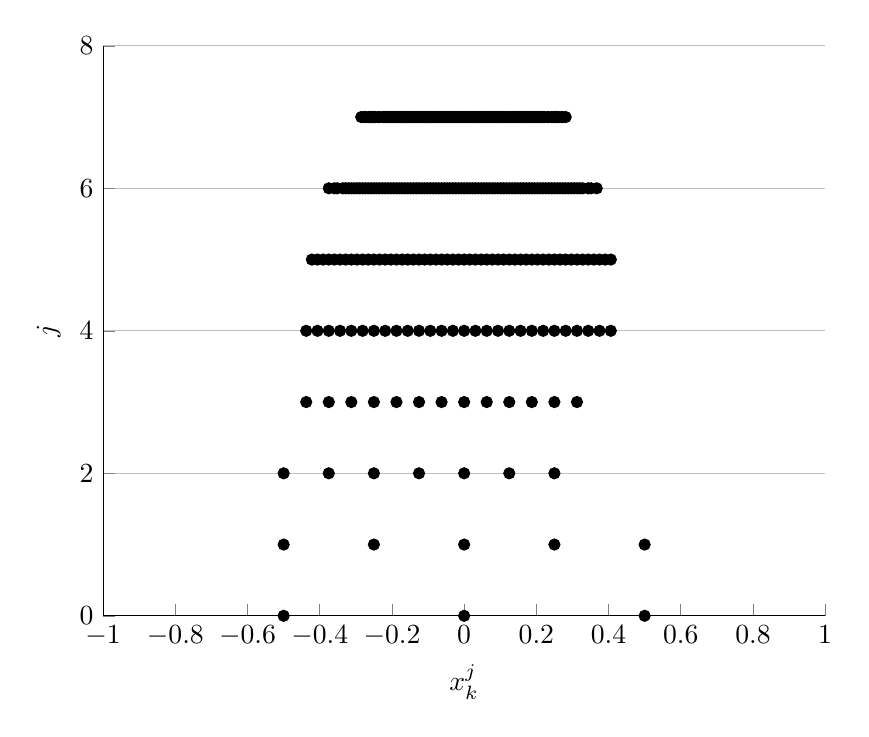
\begin{tikzpicture}

\begin{axis}[%
width=3.61in,
height=2.85in,
at={(1.01in,0.641in)},
scale only axis,
every outer x axis line/.append style={black},
every x tick label/.append style={font=\color{black}},
xmin=-1,
xmax=1,
xlabel={$x_{k}^{j}$},
every outer y axis line/.append style={black},
every y tick label/.append style={font=\color{black}},
ymin=0,
ymax=8,
ylabel={$j$},
ymajorgrids,
axis background/.style={fill=white},
axis x line*=bottom,
axis y line*=left
]
\addplot [color=black,only marks,mark=*,mark options={solid,fill=black,draw=black},forget plot]
  table[row sep=crcr]{%
-0.5	0\\
0	0\\
0.5	0\\
};
\addplot [color=black,only marks,mark=*,mark options={solid,fill=black,draw=black},forget plot]
  table[row sep=crcr]{%
-0.5	1\\
-0.25	1\\
0	1\\
0.25	1\\
0.5	1\\
};
\addplot [color=black,only marks,mark=*,mark options={solid,fill=black,draw=black},forget plot]
  table[row sep=crcr]{%
-0.5	2\\
-0.375	2\\
-0.25	2\\
-0.125	2\\
0	2\\
0.125	2\\
0.25	2\\
0.375	-5\\
0.5	-5\\
};
\addplot [color=black,only marks,mark=*,mark options={solid,fill=black,draw=black},forget plot]
  table[row sep=crcr]{%
-0.5	-5\\
-0.4375	3\\
-0.375	3\\
-0.3125	3\\
-0.25	3\\
-0.1875	3\\
-0.125	3\\
-0.0625	3\\
0	3\\
0.0625	3\\
0.125	3\\
0.1875	3\\
0.25	3\\
0.3125	3\\
0.375	-5\\
0.4375	-5\\
0.5	-5\\
};
\addplot [color=black,only marks,mark=*,mark options={solid,fill=black,draw=black},forget plot]
  table[row sep=crcr]{%
-0.5	-5\\
-0.46875	-5\\
-0.4375	4\\
-0.40625	4\\
-0.375	4\\
-0.34375	4\\
-0.3125	4\\
-0.28125	4\\
-0.25	4\\
-0.21875	4\\
-0.1875	4\\
-0.15625	4\\
-0.125	4\\
-0.09375	4\\
-0.0625	4\\
-0.03125	4\\
0	4\\
0.03125	4\\
0.0625	4\\
0.09375	4\\
0.125	4\\
0.15625	4\\
0.1875	4\\
0.21875	4\\
0.25	4\\
0.28125	4\\
0.3125	4\\
0.34375	4\\
0.375	4\\
0.40625	4\\
0.4375	-5\\
0.46875	-5\\
0.5	-5\\
};
\addplot [color=black,only marks,mark=*,mark options={solid,fill=black,draw=black},forget plot]
  table[row sep=crcr]{%
-0.5	-5\\
-0.484375	-5\\
-0.46875	-5\\
-0.453125	-5\\
-0.4375	-5\\
-0.421875	5\\
-0.40625	5\\
-0.390625	5\\
-0.375	5\\
-0.359375	5\\
-0.34375	5\\
-0.328125	5\\
-0.3125	5\\
-0.296875	5\\
-0.28125	5\\
-0.265625	5\\
-0.25	5\\
-0.234375	5\\
-0.21875	5\\
-0.203125	5\\
-0.1875	5\\
-0.171875	5\\
-0.15625	5\\
-0.140625	5\\
-0.125	5\\
-0.109375	5\\
-0.09375	5\\
-0.078125	5\\
-0.0625	5\\
-0.046875	5\\
-0.03125	5\\
-0.015625	5\\
0	5\\
0.015625	5\\
0.03125	5\\
0.046875	5\\
0.0625	5\\
0.078125	5\\
0.09375	5\\
0.109375	5\\
0.125	5\\
0.140625	5\\
0.15625	5\\
0.171875	5\\
0.1875	5\\
0.203125	5\\
0.21875	5\\
0.234375	5\\
0.25	5\\
0.265625	5\\
0.28125	5\\
0.296875	5\\
0.3125	5\\
0.328125	5\\
0.34375	5\\
0.359375	5\\
0.375	5\\
0.390625	5\\
0.40625	5\\
0.421875	-5\\
0.4375	-5\\
0.453125	-5\\
0.46875	-5\\
0.484375	-5\\
0.5	-5\\
};
\addplot [color=black,only marks,mark=*,mark options={solid,fill=black,draw=black},forget plot]
  table[row sep=crcr]{%
-0.5	-5\\
-0.492188	-5\\
-0.484375	-5\\
-0.476562	-5\\
-0.46875	-5\\
-0.460938	-5\\
-0.453125	-5\\
-0.445312	-5\\
-0.4375	-5\\
-0.429688	-5\\
-0.421875	-5\\
-0.414062	-5\\
-0.40625	-5\\
-0.398438	-5\\
-0.390625	-5\\
-0.382812	-5\\
-0.375	6\\
-0.367188	-5\\
-0.359375	6\\
-0.351562	6\\
-0.34375	-5\\
-0.335938	6\\
-0.328125	6\\
-0.320312	6\\
-0.3125	6\\
-0.304688	6\\
-0.296875	6\\
-0.289062	6\\
-0.28125	6\\
-0.273438	6\\
-0.265625	6\\
-0.257812	6\\
-0.25	6\\
-0.242188	6\\
-0.234375	6\\
-0.226562	6\\
-0.21875	6\\
-0.210938	6\\
-0.203125	6\\
-0.195312	6\\
-0.1875	6\\
-0.179688	6\\
-0.171875	6\\
-0.164062	6\\
-0.15625	6\\
-0.148438	6\\
-0.140625	6\\
-0.132812	6\\
-0.125	6\\
-0.117188	6\\
-0.109375	6\\
-0.101562	6\\
-0.09375	6\\
-0.0859375	6\\
-0.078125	6\\
-0.0703125	6\\
-0.0625	6\\
-0.0546875	6\\
-0.046875	6\\
-0.0390625	6\\
-0.03125	6\\
-0.0234375	6\\
-0.015625	6\\
-0.0078125	6\\
0	6\\
0.0078125	6\\
0.015625	6\\
0.0234375	6\\
0.03125	6\\
0.0390625	6\\
0.046875	6\\
0.0546875	6\\
0.0625	6\\
0.0703125	6\\
0.078125	6\\
0.0859375	6\\
0.09375	6\\
0.101562	6\\
0.109375	6\\
0.117188	6\\
0.125	6\\
0.132812	6\\
0.140625	6\\
0.148438	6\\
0.15625	6\\
0.164062	6\\
0.171875	6\\
0.179688	6\\
0.1875	6\\
0.195312	6\\
0.203125	6\\
0.210938	6\\
0.21875	6\\
0.226562	6\\
0.234375	6\\
0.242188	6\\
0.25	6\\
0.257812	6\\
0.265625	6\\
0.273438	6\\
0.28125	6\\
0.289062	6\\
0.296875	6\\
0.304688	6\\
0.3125	6\\
0.320312	6\\
0.328125	6\\
0.335938	-5\\
0.34375	6\\
0.351562	6\\
0.359375	-5\\
0.367188	6\\
0.375	-5\\
0.382812	-5\\
0.390625	-5\\
0.398438	-5\\
0.40625	-5\\
0.414062	-5\\
0.421875	-5\\
0.429688	-5\\
0.4375	-5\\
0.445312	-5\\
0.453125	-5\\
0.460938	-5\\
0.46875	-5\\
0.476562	-5\\
0.484375	-5\\
0.492188	-5\\
0.5	-5\\
};
\addplot [color=black,only marks,mark=*,mark options={solid,fill=black,draw=black},forget plot]
  table[row sep=crcr]{%
-0.5	-5\\
-0.496094	-5\\
-0.492188	-5\\
-0.488281	-5\\
-0.484375	-5\\
-0.480469	-5\\
-0.476562	-5\\
-0.472656	-5\\
-0.46875	-5\\
-0.464844	-5\\
-0.460938	-5\\
-0.457031	-5\\
-0.453125	-5\\
-0.449219	-5\\
-0.445312	-5\\
-0.441406	-5\\
-0.4375	-5\\
-0.433594	-5\\
-0.429688	-5\\
-0.425781	-5\\
-0.421875	-5\\
-0.417969	-5\\
-0.414062	-5\\
-0.410156	-5\\
-0.40625	-5\\
-0.402344	-5\\
-0.398438	-5\\
-0.394531	-5\\
-0.390625	-5\\
-0.386719	-5\\
-0.382812	-5\\
-0.378906	-5\\
-0.375	-5\\
-0.371094	-5\\
-0.367188	-5\\
-0.363281	-5\\
-0.359375	-5\\
-0.355469	-5\\
-0.351562	-5\\
-0.347656	-5\\
-0.34375	-5\\
-0.339844	-5\\
-0.335938	-5\\
-0.332031	-5\\
-0.328125	-5\\
-0.324219	-5\\
-0.320312	-5\\
-0.316406	-5\\
-0.3125	-5\\
-0.308594	-5\\
-0.304688	-5\\
-0.300781	-5\\
-0.296875	-5\\
-0.292969	-5\\
-0.289062	-5\\
-0.285156	7\\
-0.28125	-5\\
-0.277344	7\\
-0.273438	7\\
-0.269531	-5\\
-0.265625	7\\
-0.261719	7\\
-0.257812	7\\
-0.253906	7\\
-0.25	7\\
-0.246094	7\\
-0.242188	-5\\
-0.238281	7\\
-0.234375	7\\
-0.230469	-5\\
-0.226562	7\\
-0.222656	7\\
-0.21875	7\\
-0.214844	7\\
-0.210938	7\\
-0.207031	7\\
-0.203125	7\\
-0.199219	7\\
-0.195312	7\\
-0.191406	7\\
-0.1875	7\\
-0.183594	7\\
-0.179688	7\\
-0.175781	7\\
-0.171875	7\\
-0.167969	7\\
-0.164062	7\\
-0.160156	7\\
-0.15625	7\\
-0.152344	7\\
-0.148438	7\\
-0.144531	7\\
-0.140625	7\\
-0.136719	7\\
-0.132812	7\\
-0.128906	7\\
-0.125	7\\
-0.121094	7\\
-0.117188	7\\
-0.113281	7\\
-0.109375	7\\
-0.105469	7\\
-0.101562	7\\
-0.0976562	7\\
-0.09375	7\\
-0.0898438	7\\
-0.0859375	7\\
-0.0820312	7\\
-0.078125	7\\
-0.0742188	7\\
-0.0703125	7\\
-0.0664062	7\\
-0.0625	7\\
-0.0585938	7\\
-0.0546875	7\\
-0.0507812	7\\
-0.046875	7\\
-0.0429688	7\\
-0.0390625	7\\
-0.0351562	7\\
-0.03125	7\\
-0.0273438	7\\
-0.0234375	7\\
-0.0195312	7\\
-0.015625	7\\
-0.0117188	7\\
-0.0078125	7\\
-0.00390625	7\\
0	7\\
0.00390625	7\\
0.0078125	7\\
0.0117188	7\\
0.015625	7\\
0.0195312	7\\
0.0234375	7\\
0.0273438	7\\
0.03125	7\\
0.0351562	7\\
0.0390625	7\\
0.0429688	7\\
0.046875	7\\
0.0507812	7\\
0.0546875	7\\
0.0585938	7\\
0.0625	7\\
0.0664062	7\\
0.0703125	7\\
0.0742188	7\\
0.078125	7\\
0.0820312	7\\
0.0859375	7\\
0.0898438	7\\
0.09375	7\\
0.0976562	7\\
0.101562	7\\
0.105469	7\\
0.109375	7\\
0.113281	7\\
0.117188	7\\
0.121094	7\\
0.125	7\\
0.128906	7\\
0.132812	7\\
0.136719	7\\
0.140625	7\\
0.144531	7\\
0.148438	7\\
0.152344	7\\
0.15625	7\\
0.160156	7\\
0.164062	7\\
0.167969	7\\
0.171875	7\\
0.175781	7\\
0.179688	7\\
0.183594	7\\
0.1875	7\\
0.191406	7\\
0.195312	7\\
0.199219	7\\
0.203125	7\\
0.207031	7\\
0.210938	7\\
0.214844	7\\
0.21875	7\\
0.222656	7\\
0.226562	-5\\
0.230469	7\\
0.234375	7\\
0.238281	-5\\
0.242188	7\\
0.246094	7\\
0.25	7\\
0.253906	7\\
0.257812	7\\
0.261719	7\\
0.265625	-5\\
0.269531	7\\
0.273438	7\\
0.277344	-5\\
0.28125	7\\
0.285156	-5\\
0.289062	-5\\
0.292969	-5\\
0.296875	-5\\
0.300781	-5\\
0.304688	-5\\
0.308594	-5\\
0.3125	-5\\
0.316406	-5\\
0.320312	-5\\
0.324219	-5\\
0.328125	-5\\
0.332031	-5\\
0.335938	-5\\
0.339844	-5\\
0.34375	-5\\
0.347656	-5\\
0.351562	-5\\
0.355469	-5\\
0.359375	-5\\
0.363281	-5\\
0.367188	-5\\
0.371094	-5\\
0.375	-5\\
0.378906	-5\\
0.382812	-5\\
0.386719	-5\\
0.390625	-5\\
0.394531	-5\\
0.398438	-5\\
0.402344	-5\\
0.40625	-5\\
0.410156	-5\\
0.414062	-5\\
0.417969	-5\\
0.421875	-5\\
0.425781	-5\\
0.429688	-5\\
0.433594	-5\\
0.4375	-5\\
0.441406	-5\\
0.445312	-5\\
0.449219	-5\\
0.453125	-5\\
0.457031	-5\\
0.460938	-5\\
0.464844	-5\\
0.46875	-5\\
0.472656	-5\\
0.476562	-5\\
0.480469	-5\\
0.484375	-5\\
0.488281	-5\\
0.492188	-5\\
0.496094	-5\\
0.5	-5\\
};
\addplot [color=black,only marks,mark=*,mark options={solid,fill=black,draw=black},forget plot]
  table[row sep=crcr]{%
-0.5	-5\\
-0.498047	-5\\
-0.496094	-5\\
-0.494141	-5\\
-0.492188	-5\\
-0.490234	-5\\
-0.488281	-5\\
-0.486328	-5\\
-0.484375	-5\\
-0.482422	-5\\
-0.480469	-5\\
-0.478516	-5\\
-0.476562	-5\\
-0.474609	-5\\
-0.472656	-5\\
-0.470703	-5\\
-0.46875	-5\\
-0.466797	-5\\
-0.464844	-5\\
-0.462891	-5\\
-0.460938	-5\\
-0.458984	-5\\
-0.457031	-5\\
-0.455078	-5\\
-0.453125	-5\\
-0.451172	-5\\
-0.449219	-5\\
-0.447266	-5\\
-0.445312	-5\\
-0.443359	-5\\
-0.441406	-5\\
-0.439453	-5\\
-0.4375	-5\\
-0.435547	-5\\
-0.433594	-5\\
-0.431641	-5\\
-0.429688	-5\\
-0.427734	-5\\
-0.425781	-5\\
-0.423828	-5\\
-0.421875	-5\\
-0.419922	-5\\
-0.417969	-5\\
-0.416016	-5\\
-0.414062	-5\\
-0.412109	-5\\
-0.410156	-5\\
-0.408203	-5\\
-0.40625	-5\\
-0.404297	-5\\
-0.402344	-5\\
-0.400391	-5\\
-0.398438	-5\\
-0.396484	-5\\
-0.394531	-5\\
-0.392578	-5\\
-0.390625	-5\\
-0.388672	-5\\
-0.386719	-5\\
-0.384766	-5\\
-0.382812	-5\\
-0.380859	-5\\
-0.378906	-5\\
-0.376953	-5\\
-0.375	-5\\
-0.373047	-5\\
-0.371094	-5\\
-0.369141	-5\\
-0.367188	-5\\
-0.365234	-5\\
-0.363281	-5\\
-0.361328	-5\\
-0.359375	-5\\
-0.357422	-5\\
-0.355469	-5\\
-0.353516	-5\\
-0.351562	-5\\
-0.349609	-5\\
-0.347656	-5\\
-0.345703	-5\\
-0.34375	-5\\
-0.341797	-5\\
-0.339844	-5\\
-0.337891	-5\\
-0.335938	-5\\
-0.333984	-5\\
-0.332031	-5\\
-0.330078	-5\\
-0.328125	-5\\
-0.326172	-5\\
-0.324219	-5\\
-0.322266	-5\\
-0.320312	-5\\
-0.318359	-5\\
-0.316406	-5\\
-0.314453	-5\\
-0.3125	-5\\
-0.310547	-5\\
-0.308594	-5\\
-0.306641	-5\\
-0.304688	-5\\
-0.302734	-5\\
-0.300781	-5\\
-0.298828	-5\\
-0.296875	-5\\
-0.294922	-5\\
-0.292969	-5\\
-0.291016	-5\\
-0.289062	-5\\
-0.287109	-5\\
-0.285156	-5\\
-0.283203	-5\\
-0.28125	-5\\
-0.279297	-5\\
-0.277344	-5\\
-0.275391	-5\\
-0.273438	-5\\
-0.271484	-5\\
-0.269531	-5\\
-0.267578	-5\\
-0.265625	-5\\
-0.263672	-5\\
-0.261719	-5\\
-0.259766	-5\\
-0.257812	-5\\
-0.255859	-5\\
-0.253906	-5\\
-0.251953	-5\\
-0.25	-5\\
-0.248047	-5\\
-0.246094	-5\\
-0.244141	-5\\
-0.242188	-5\\
-0.240234	-5\\
-0.238281	-5\\
-0.236328	-5\\
-0.234375	-5\\
-0.232422	-5\\
-0.230469	-5\\
-0.228516	-5\\
-0.226562	-5\\
-0.224609	-5\\
-0.222656	-5\\
-0.220703	-5\\
-0.21875	-5\\
-0.216797	-5\\
-0.214844	-5\\
-0.212891	-5\\
-0.210938	-5\\
-0.208984	-5\\
-0.207031	-5\\
-0.205078	-5\\
-0.203125	-5\\
-0.201172	-5\\
-0.199219	-5\\
-0.197266	-5\\
-0.195312	-5\\
-0.193359	-5\\
-0.191406	-5\\
-0.189453	-5\\
-0.1875	-5\\
-0.185547	-5\\
-0.183594	-5\\
-0.181641	-5\\
-0.179688	-5\\
-0.177734	-5\\
-0.175781	-5\\
-0.173828	-5\\
-0.171875	-5\\
-0.169922	-5\\
-0.167969	-5\\
-0.166016	-5\\
-0.164062	-5\\
-0.162109	-5\\
-0.160156	-5\\
-0.158203	-5\\
-0.15625	-5\\
-0.154297	-5\\
-0.152344	-5\\
-0.150391	-5\\
-0.148438	-5\\
-0.146484	-5\\
-0.144531	-5\\
-0.142578	-5\\
-0.140625	-5\\
-0.138672	-5\\
-0.136719	-5\\
-0.134766	-5\\
-0.132812	-5\\
-0.130859	-5\\
-0.128906	-5\\
-0.126953	-5\\
-0.125	-5\\
-0.123047	-5\\
-0.121094	-5\\
-0.119141	-5\\
-0.117188	-5\\
-0.115234	-5\\
-0.113281	-5\\
-0.111328	-5\\
-0.109375	-5\\
-0.107422	-5\\
-0.105469	-5\\
-0.103516	-5\\
-0.101562	-5\\
-0.0996094	-5\\
-0.0976562	-5\\
-0.0957031	-5\\
-0.09375	-5\\
-0.0917969	-5\\
-0.0898438	-5\\
-0.0878906	-5\\
-0.0859375	-5\\
-0.0839844	-5\\
-0.0820312	-5\\
-0.0800781	-5\\
-0.078125	-5\\
-0.0761719	-5\\
-0.0742188	-5\\
-0.0722656	-5\\
-0.0703125	-5\\
-0.0683594	-5\\
-0.0664062	-5\\
-0.0644531	-5\\
-0.0625	-5\\
-0.0605469	-5\\
-0.0585938	-5\\
-0.0566406	-5\\
-0.0546875	-5\\
-0.0527344	-5\\
-0.0507812	-5\\
-0.0488281	-5\\
-0.046875	-5\\
-0.0449219	-5\\
-0.0429688	-5\\
-0.0410156	-5\\
-0.0390625	-5\\
-0.0371094	-5\\
-0.0351562	-5\\
-0.0332031	-5\\
-0.03125	-5\\
-0.0292969	-5\\
-0.0273438	-5\\
-0.0253906	-5\\
-0.0234375	-5\\
-0.0214844	-5\\
-0.0195312	-5\\
-0.0175781	-5\\
-0.015625	-5\\
-0.0136719	-5\\
-0.0117188	-5\\
-0.00976562	-5\\
-0.0078125	-5\\
-0.00585938	-5\\
-0.00390625	-5\\
-0.00195312	-5\\
0	-5\\
0.00195312	-5\\
0.00390625	-5\\
0.00585938	-5\\
0.0078125	-5\\
0.00976562	-5\\
0.0117188	-5\\
0.0136719	-5\\
0.015625	-5\\
0.0175781	-5\\
0.0195312	-5\\
0.0214844	-5\\
0.0234375	-5\\
0.0253906	-5\\
0.0273438	-5\\
0.0292969	-5\\
0.03125	-5\\
0.0332031	-5\\
0.0351562	-5\\
0.0371094	-5\\
0.0390625	-5\\
0.0410156	-5\\
0.0429688	-5\\
0.0449219	-5\\
0.046875	-5\\
0.0488281	-5\\
0.0507812	-5\\
0.0527344	-5\\
0.0546875	-5\\
0.0566406	-5\\
0.0585938	-5\\
0.0605469	-5\\
0.0625	-5\\
0.0644531	-5\\
0.0664062	-5\\
0.0683594	-5\\
0.0703125	-5\\
0.0722656	-5\\
0.0742188	-5\\
0.0761719	-5\\
0.078125	-5\\
0.0800781	-5\\
0.0820312	-5\\
0.0839844	-5\\
0.0859375	-5\\
0.0878906	-5\\
0.0898438	-5\\
0.0917969	-5\\
0.09375	-5\\
0.0957031	-5\\
0.0976562	-5\\
0.0996094	-5\\
0.101562	-5\\
0.103516	-5\\
0.105469	-5\\
0.107422	-5\\
0.109375	-5\\
0.111328	-5\\
0.113281	-5\\
0.115234	-5\\
0.117188	-5\\
0.119141	-5\\
0.121094	-5\\
0.123047	-5\\
0.125	-5\\
0.126953	-5\\
0.128906	-5\\
0.130859	-5\\
0.132812	-5\\
0.134766	-5\\
0.136719	-5\\
0.138672	-5\\
0.140625	-5\\
0.142578	-5\\
0.144531	-5\\
0.146484	-5\\
0.148438	-5\\
0.150391	-5\\
0.152344	-5\\
0.154297	-5\\
0.15625	-5\\
0.158203	-5\\
0.160156	-5\\
0.162109	-5\\
0.164062	-5\\
0.166016	-5\\
0.167969	-5\\
0.169922	-5\\
0.171875	-5\\
0.173828	-5\\
0.175781	-5\\
0.177734	-5\\
0.179688	-5\\
0.181641	-5\\
0.183594	-5\\
0.185547	-5\\
0.1875	-5\\
0.189453	-5\\
0.191406	-5\\
0.193359	-5\\
0.195312	-5\\
0.197266	-5\\
0.199219	-5\\
0.201172	-5\\
0.203125	-5\\
0.205078	-5\\
0.207031	-5\\
0.208984	-5\\
0.210938	-5\\
0.212891	-5\\
0.214844	-5\\
0.216797	-5\\
0.21875	-5\\
0.220703	-5\\
0.222656	-5\\
0.224609	-5\\
0.226562	-5\\
0.228516	-5\\
0.230469	-5\\
0.232422	-5\\
0.234375	-5\\
0.236328	-5\\
0.238281	-5\\
0.240234	-5\\
0.242188	-5\\
0.244141	-5\\
0.246094	-5\\
0.248047	-5\\
0.25	-5\\
0.251953	-5\\
0.253906	-5\\
0.255859	-5\\
0.257812	-5\\
0.259766	-5\\
0.261719	-5\\
0.263672	-5\\
0.265625	-5\\
0.267578	-5\\
0.269531	-5\\
0.271484	-5\\
0.273438	-5\\
0.275391	-5\\
0.277344	-5\\
0.279297	-5\\
0.28125	-5\\
0.283203	-5\\
0.285156	-5\\
0.287109	-5\\
0.289062	-5\\
0.291016	-5\\
0.292969	-5\\
0.294922	-5\\
0.296875	-5\\
0.298828	-5\\
0.300781	-5\\
0.302734	-5\\
0.304688	-5\\
0.306641	-5\\
0.308594	-5\\
0.310547	-5\\
0.3125	-5\\
0.314453	-5\\
0.316406	-5\\
0.318359	-5\\
0.320312	-5\\
0.322266	-5\\
0.324219	-5\\
0.326172	-5\\
0.328125	-5\\
0.330078	-5\\
0.332031	-5\\
0.333984	-5\\
0.335938	-5\\
0.337891	-5\\
0.339844	-5\\
0.341797	-5\\
0.34375	-5\\
0.345703	-5\\
0.347656	-5\\
0.349609	-5\\
0.351562	-5\\
0.353516	-5\\
0.355469	-5\\
0.357422	-5\\
0.359375	-5\\
0.361328	-5\\
0.363281	-5\\
0.365234	-5\\
0.367188	-5\\
0.369141	-5\\
0.371094	-5\\
0.373047	-5\\
0.375	-5\\
0.376953	-5\\
0.378906	-5\\
0.380859	-5\\
0.382812	-5\\
0.384766	-5\\
0.386719	-5\\
0.388672	-5\\
0.390625	-5\\
0.392578	-5\\
0.394531	-5\\
0.396484	-5\\
0.398438	-5\\
0.400391	-5\\
0.402344	-5\\
0.404297	-5\\
0.40625	-5\\
0.408203	-5\\
0.410156	-5\\
0.412109	-5\\
0.414062	-5\\
0.416016	-5\\
0.417969	-5\\
0.419922	-5\\
0.421875	-5\\
0.423828	-5\\
0.425781	-5\\
0.427734	-5\\
0.429688	-5\\
0.431641	-5\\
0.433594	-5\\
0.435547	-5\\
0.4375	-5\\
0.439453	-5\\
0.441406	-5\\
0.443359	-5\\
0.445312	-5\\
0.447266	-5\\
0.449219	-5\\
0.451172	-5\\
0.453125	-5\\
0.455078	-5\\
0.457031	-5\\
0.458984	-5\\
0.460938	-5\\
0.462891	-5\\
0.464844	-5\\
0.466797	-5\\
0.46875	-5\\
0.470703	-5\\
0.472656	-5\\
0.474609	-5\\
0.476562	-5\\
0.478516	-5\\
0.480469	-5\\
0.482422	-5\\
0.484375	-5\\
0.486328	-5\\
0.488281	-5\\
0.490234	-5\\
0.492188	-5\\
0.494141	-5\\
0.496094	-5\\
0.498047	-5\\
0.5	-5\\
};
\end{axis}
\end{tikzpicture}%
	\caption{Coefficients kept with $\epsilon=10^{-5}$.}
\end{figure}

\begin{figure}[H]
	\center
	% GNUPLOT: LaTeX picture
\setlength{\unitlength}{0.240900pt}
\ifx\plotpoint\undefined\newsavebox{\plotpoint}\fi
\sbox{\plotpoint}{\rule[-0.200pt]{0.400pt}{0.400pt}}%
\begin{picture}(1500,900)(0,0)
\sbox{\plotpoint}{\rule[-0.200pt]{0.400pt}{0.400pt}}%
\put(171.0,131.0){\rule[-0.200pt]{4.818pt}{0.400pt}}
\put(151,131){\makebox(0,0)[r]{$-1$}}
\put(1419.0,131.0){\rule[-0.200pt]{4.818pt}{0.400pt}}
\put(171.0,204.0){\rule[-0.200pt]{4.818pt}{0.400pt}}
\put(151,204){\makebox(0,0)[r]{$-0.8$}}
\put(1419.0,204.0){\rule[-0.200pt]{4.818pt}{0.400pt}}
\put(171.0,277.0){\rule[-0.200pt]{4.818pt}{0.400pt}}
\put(151,277){\makebox(0,0)[r]{$-0.6$}}
\put(1419.0,277.0){\rule[-0.200pt]{4.818pt}{0.400pt}}
\put(171.0,349.0){\rule[-0.200pt]{4.818pt}{0.400pt}}
\put(151,349){\makebox(0,0)[r]{$-0.4$}}
\put(1419.0,349.0){\rule[-0.200pt]{4.818pt}{0.400pt}}
\put(171.0,422.0){\rule[-0.200pt]{4.818pt}{0.400pt}}
\put(151,422){\makebox(0,0)[r]{$-0.2$}}
\put(1419.0,422.0){\rule[-0.200pt]{4.818pt}{0.400pt}}
\put(171.0,495.0){\rule[-0.200pt]{4.818pt}{0.400pt}}
\put(151,495){\makebox(0,0)[r]{$0$}}
\put(1419.0,495.0){\rule[-0.200pt]{4.818pt}{0.400pt}}
\put(171.0,568.0){\rule[-0.200pt]{4.818pt}{0.400pt}}
\put(151,568){\makebox(0,0)[r]{$0.2$}}
\put(1419.0,568.0){\rule[-0.200pt]{4.818pt}{0.400pt}}
\put(171.0,641.0){\rule[-0.200pt]{4.818pt}{0.400pt}}
\put(151,641){\makebox(0,0)[r]{$0.4$}}
\put(1419.0,641.0){\rule[-0.200pt]{4.818pt}{0.400pt}}
\put(171.0,713.0){\rule[-0.200pt]{4.818pt}{0.400pt}}
\put(151,713){\makebox(0,0)[r]{$0.6$}}
\put(1419.0,713.0){\rule[-0.200pt]{4.818pt}{0.400pt}}
\put(171.0,786.0){\rule[-0.200pt]{4.818pt}{0.400pt}}
\put(151,786){\makebox(0,0)[r]{$0.8$}}
\put(1419.0,786.0){\rule[-0.200pt]{4.818pt}{0.400pt}}
\put(171.0,859.0){\rule[-0.200pt]{4.818pt}{0.400pt}}
\put(151,859){\makebox(0,0)[r]{$1$}}
\put(1419.0,859.0){\rule[-0.200pt]{4.818pt}{0.400pt}}
\put(171.0,131.0){\rule[-0.200pt]{0.400pt}{4.818pt}}
\put(171,90){\makebox(0,0){$-0.6$}}
\put(171.0,839.0){\rule[-0.200pt]{0.400pt}{4.818pt}}
\put(382.0,131.0){\rule[-0.200pt]{0.400pt}{4.818pt}}
\put(382,90){\makebox(0,0){$-0.4$}}
\put(382.0,839.0){\rule[-0.200pt]{0.400pt}{4.818pt}}
\put(594.0,131.0){\rule[-0.200pt]{0.400pt}{4.818pt}}
\put(594,90){\makebox(0,0){$-0.2$}}
\put(594.0,839.0){\rule[-0.200pt]{0.400pt}{4.818pt}}
\put(805.0,131.0){\rule[-0.200pt]{0.400pt}{4.818pt}}
\put(805,90){\makebox(0,0){$0$}}
\put(805.0,839.0){\rule[-0.200pt]{0.400pt}{4.818pt}}
\put(1016.0,131.0){\rule[-0.200pt]{0.400pt}{4.818pt}}
\put(1016,90){\makebox(0,0){$0.2$}}
\put(1016.0,839.0){\rule[-0.200pt]{0.400pt}{4.818pt}}
\put(1228.0,131.0){\rule[-0.200pt]{0.400pt}{4.818pt}}
\put(1228,90){\makebox(0,0){$0.4$}}
\put(1228.0,839.0){\rule[-0.200pt]{0.400pt}{4.818pt}}
\put(1439.0,131.0){\rule[-0.200pt]{0.400pt}{4.818pt}}
\put(1439,90){\makebox(0,0){$0.6$}}
\put(1439.0,839.0){\rule[-0.200pt]{0.400pt}{4.818pt}}
\put(171.0,131.0){\rule[-0.200pt]{0.400pt}{175.375pt}}
\put(171.0,131.0){\rule[-0.200pt]{305.461pt}{0.400pt}}
\put(1439.0,131.0){\rule[-0.200pt]{0.400pt}{175.375pt}}
\put(171.0,859.0){\rule[-0.200pt]{305.461pt}{0.400pt}}
\put(30,495){\makebox(0,0){$f(x)$}}
\put(805,29){\makebox(0,0){$x$}}
\put(277,495){\usebox{\plotpoint}}
\put(460,493.67){\rule{0.482pt}{0.400pt}}
\multiput(460.00,494.17)(1.000,-1.000){2}{\rule{0.241pt}{0.400pt}}
\put(277.0,495.0){\rule[-0.200pt]{44.085pt}{0.400pt}}
\put(477,493.67){\rule{0.482pt}{0.400pt}}
\multiput(477.00,493.17)(1.000,1.000){2}{\rule{0.241pt}{0.400pt}}
\put(462.0,494.0){\rule[-0.200pt]{3.613pt}{0.400pt}}
\put(485,494.67){\rule{0.482pt}{0.400pt}}
\multiput(485.00,494.17)(1.000,1.000){2}{\rule{0.241pt}{0.400pt}}
\put(479.0,495.0){\rule[-0.200pt]{1.445pt}{0.400pt}}
\put(491,494.67){\rule{0.482pt}{0.400pt}}
\multiput(491.00,495.17)(1.000,-1.000){2}{\rule{0.241pt}{0.400pt}}
\put(487.0,496.0){\rule[-0.200pt]{0.964pt}{0.400pt}}
\put(495,493.67){\rule{0.482pt}{0.400pt}}
\multiput(495.00,494.17)(1.000,-1.000){2}{\rule{0.241pt}{0.400pt}}
\put(497,492.67){\rule{0.723pt}{0.400pt}}
\multiput(497.00,493.17)(1.500,-1.000){2}{\rule{0.361pt}{0.400pt}}
\put(493.0,495.0){\rule[-0.200pt]{0.482pt}{0.400pt}}
\put(502,492.67){\rule{0.482pt}{0.400pt}}
\multiput(502.00,492.17)(1.000,1.000){2}{\rule{0.241pt}{0.400pt}}
\put(500.0,493.0){\rule[-0.200pt]{0.482pt}{0.400pt}}
\put(506,493.67){\rule{0.482pt}{0.400pt}}
\multiput(506.00,493.17)(1.000,1.000){2}{\rule{0.241pt}{0.400pt}}
\put(508,494.67){\rule{0.482pt}{0.400pt}}
\multiput(508.00,494.17)(1.000,1.000){2}{\rule{0.241pt}{0.400pt}}
\put(510,495.67){\rule{0.482pt}{0.400pt}}
\multiput(510.00,495.17)(1.000,1.000){2}{\rule{0.241pt}{0.400pt}}
\put(512,496.67){\rule{0.482pt}{0.400pt}}
\multiput(512.00,496.17)(1.000,1.000){2}{\rule{0.241pt}{0.400pt}}
\put(504.0,494.0){\rule[-0.200pt]{0.482pt}{0.400pt}}
\put(516,496.67){\rule{0.482pt}{0.400pt}}
\multiput(516.00,497.17)(1.000,-1.000){2}{\rule{0.241pt}{0.400pt}}
\put(518,495.17){\rule{0.482pt}{0.400pt}}
\multiput(518.00,496.17)(1.000,-2.000){2}{\rule{0.241pt}{0.400pt}}
\put(520,493.67){\rule{0.482pt}{0.400pt}}
\multiput(520.00,494.17)(1.000,-1.000){2}{\rule{0.241pt}{0.400pt}}
\put(522,492.17){\rule{0.482pt}{0.400pt}}
\multiput(522.00,493.17)(1.000,-2.000){2}{\rule{0.241pt}{0.400pt}}
\put(524,490.67){\rule{0.482pt}{0.400pt}}
\multiput(524.00,491.17)(1.000,-1.000){2}{\rule{0.241pt}{0.400pt}}
\put(514.0,498.0){\rule[-0.200pt]{0.482pt}{0.400pt}}
\put(528,490.67){\rule{0.723pt}{0.400pt}}
\multiput(528.00,490.17)(1.500,1.000){2}{\rule{0.361pt}{0.400pt}}
\put(531,491.67){\rule{0.482pt}{0.400pt}}
\multiput(531.00,491.17)(1.000,1.000){2}{\rule{0.241pt}{0.400pt}}
\put(533,493.17){\rule{0.482pt}{0.400pt}}
\multiput(533.00,492.17)(1.000,2.000){2}{\rule{0.241pt}{0.400pt}}
\put(535.17,495){\rule{0.400pt}{0.700pt}}
\multiput(534.17,495.00)(2.000,1.547){2}{\rule{0.400pt}{0.350pt}}
\put(537.17,498){\rule{0.400pt}{0.700pt}}
\multiput(536.17,498.00)(2.000,1.547){2}{\rule{0.400pt}{0.350pt}}
\put(539,500.67){\rule{0.482pt}{0.400pt}}
\multiput(539.00,500.17)(1.000,1.000){2}{\rule{0.241pt}{0.400pt}}
\put(541,500.67){\rule{0.482pt}{0.400pt}}
\multiput(541.00,501.17)(1.000,-1.000){2}{\rule{0.241pt}{0.400pt}}
\put(543,499.17){\rule{0.482pt}{0.400pt}}
\multiput(543.00,500.17)(1.000,-2.000){2}{\rule{0.241pt}{0.400pt}}
\put(545.17,496){\rule{0.400pt}{0.700pt}}
\multiput(544.17,497.55)(2.000,-1.547){2}{\rule{0.400pt}{0.350pt}}
\put(547.17,492){\rule{0.400pt}{0.900pt}}
\multiput(546.17,494.13)(2.000,-2.132){2}{\rule{0.400pt}{0.450pt}}
\put(549.17,488){\rule{0.400pt}{0.900pt}}
\multiput(548.17,490.13)(2.000,-2.132){2}{\rule{0.400pt}{0.450pt}}
\put(551,486.17){\rule{0.482pt}{0.400pt}}
\multiput(551.00,487.17)(1.000,-2.000){2}{\rule{0.241pt}{0.400pt}}
\put(553,484.67){\rule{0.482pt}{0.400pt}}
\multiput(553.00,485.17)(1.000,-1.000){2}{\rule{0.241pt}{0.400pt}}
\put(555,485.17){\rule{0.482pt}{0.400pt}}
\multiput(555.00,484.17)(1.000,2.000){2}{\rule{0.241pt}{0.400pt}}
\put(557.17,487){\rule{0.400pt}{1.100pt}}
\multiput(556.17,487.00)(2.000,2.717){2}{\rule{0.400pt}{0.550pt}}
\put(559.17,492){\rule{0.400pt}{1.300pt}}
\multiput(558.17,492.00)(2.000,3.302){2}{\rule{0.400pt}{0.650pt}}
\multiput(561.61,498.00)(0.447,1.132){3}{\rule{0.108pt}{0.900pt}}
\multiput(560.17,498.00)(3.000,4.132){2}{\rule{0.400pt}{0.450pt}}
\put(564.17,504){\rule{0.400pt}{0.900pt}}
\multiput(563.17,504.00)(2.000,2.132){2}{\rule{0.400pt}{0.450pt}}
\put(566,507.67){\rule{0.482pt}{0.400pt}}
\multiput(566.00,507.17)(1.000,1.000){2}{\rule{0.241pt}{0.400pt}}
\put(568,507.67){\rule{0.482pt}{0.400pt}}
\multiput(568.00,508.17)(1.000,-1.000){2}{\rule{0.241pt}{0.400pt}}
\put(570.17,503){\rule{0.400pt}{1.100pt}}
\multiput(569.17,505.72)(2.000,-2.717){2}{\rule{0.400pt}{0.550pt}}
\put(572.17,495){\rule{0.400pt}{1.700pt}}
\multiput(571.17,499.47)(2.000,-4.472){2}{\rule{0.400pt}{0.850pt}}
\put(574.17,487){\rule{0.400pt}{1.700pt}}
\multiput(573.17,491.47)(2.000,-4.472){2}{\rule{0.400pt}{0.850pt}}
\put(576.17,479){\rule{0.400pt}{1.700pt}}
\multiput(575.17,483.47)(2.000,-4.472){2}{\rule{0.400pt}{0.850pt}}
\put(578.17,475){\rule{0.400pt}{0.900pt}}
\multiput(577.17,477.13)(2.000,-2.132){2}{\rule{0.400pt}{0.450pt}}
\put(580,474.67){\rule{0.482pt}{0.400pt}}
\multiput(580.00,474.17)(1.000,1.000){2}{\rule{0.241pt}{0.400pt}}
\put(582.17,476){\rule{0.400pt}{1.100pt}}
\multiput(581.17,476.00)(2.000,2.717){2}{\rule{0.400pt}{0.550pt}}
\put(584.17,481){\rule{0.400pt}{1.900pt}}
\multiput(583.17,481.00)(2.000,5.056){2}{\rule{0.400pt}{0.950pt}}
\put(586.17,490){\rule{0.400pt}{2.500pt}}
\multiput(585.17,490.00)(2.000,6.811){2}{\rule{0.400pt}{1.250pt}}
\put(588.17,502){\rule{0.400pt}{2.300pt}}
\multiput(587.17,502.00)(2.000,6.226){2}{\rule{0.400pt}{1.150pt}}
\put(590.17,513){\rule{0.400pt}{1.700pt}}
\multiput(589.17,513.00)(2.000,4.472){2}{\rule{0.400pt}{0.850pt}}
\put(592,521.17){\rule{0.482pt}{0.400pt}}
\multiput(592.00,520.17)(1.000,2.000){2}{\rule{0.241pt}{0.400pt}}
\multiput(594.61,519.82)(0.447,-0.909){3}{\rule{0.108pt}{0.767pt}}
\multiput(593.17,521.41)(3.000,-3.409){2}{\rule{0.400pt}{0.383pt}}
\put(597.17,507){\rule{0.400pt}{2.300pt}}
\multiput(596.17,513.23)(2.000,-6.226){2}{\rule{0.400pt}{1.150pt}}
\put(599.17,492){\rule{0.400pt}{3.100pt}}
\multiput(598.17,500.57)(2.000,-8.566){2}{\rule{0.400pt}{1.550pt}}
\put(601.17,476){\rule{0.400pt}{3.300pt}}
\multiput(600.17,485.15)(2.000,-9.151){2}{\rule{0.400pt}{1.650pt}}
\put(603.17,463){\rule{0.400pt}{2.700pt}}
\multiput(602.17,470.40)(2.000,-7.396){2}{\rule{0.400pt}{1.350pt}}
\put(605.17,457){\rule{0.400pt}{1.300pt}}
\multiput(604.17,460.30)(2.000,-3.302){2}{\rule{0.400pt}{0.650pt}}
\put(607.17,457){\rule{0.400pt}{0.700pt}}
\multiput(606.17,457.00)(2.000,1.547){2}{\rule{0.400pt}{0.350pt}}
\put(609.17,460){\rule{0.400pt}{2.500pt}}
\multiput(608.17,460.00)(2.000,6.811){2}{\rule{0.400pt}{1.250pt}}
\put(611.17,472){\rule{0.400pt}{3.900pt}}
\multiput(610.17,472.00)(2.000,10.905){2}{\rule{0.400pt}{1.950pt}}
\put(613.17,491){\rule{0.400pt}{4.500pt}}
\multiput(612.17,491.00)(2.000,12.660){2}{\rule{0.400pt}{2.250pt}}
\put(615.17,513){\rule{0.400pt}{3.900pt}}
\multiput(614.17,513.00)(2.000,10.905){2}{\rule{0.400pt}{1.950pt}}
\put(617.17,532){\rule{0.400pt}{2.500pt}}
\multiput(616.17,532.00)(2.000,6.811){2}{\rule{0.400pt}{1.250pt}}
\put(619,543.67){\rule{0.482pt}{0.400pt}}
\multiput(619.00,543.17)(1.000,1.000){2}{\rule{0.241pt}{0.400pt}}
\put(621.17,534){\rule{0.400pt}{2.300pt}}
\multiput(620.17,540.23)(2.000,-6.226){2}{\rule{0.400pt}{1.150pt}}
\put(623.17,511){\rule{0.400pt}{4.700pt}}
\multiput(622.17,524.24)(2.000,-13.245){2}{\rule{0.400pt}{2.350pt}}
\multiput(625.61,495.09)(0.447,-6.044){3}{\rule{0.108pt}{3.833pt}}
\multiput(624.17,503.04)(3.000,-20.044){2}{\rule{0.400pt}{1.917pt}}
\put(628.17,455){\rule{0.400pt}{5.700pt}}
\multiput(627.17,471.17)(2.000,-16.169){2}{\rule{0.400pt}{2.850pt}}
\put(630.17,435){\rule{0.400pt}{4.100pt}}
\multiput(629.17,446.49)(2.000,-11.490){2}{\rule{0.400pt}{2.050pt}}
\put(632.17,428){\rule{0.400pt}{1.500pt}}
\multiput(631.17,431.89)(2.000,-3.887){2}{\rule{0.400pt}{0.750pt}}
\put(634.17,428){\rule{0.400pt}{1.700pt}}
\multiput(633.17,428.00)(2.000,4.472){2}{\rule{0.400pt}{0.850pt}}
\put(636.17,436){\rule{0.400pt}{5.100pt}}
\multiput(635.17,436.00)(2.000,14.415){2}{\rule{0.400pt}{2.550pt}}
\put(638.17,461){\rule{0.400pt}{6.900pt}}
\multiput(637.17,461.00)(2.000,19.679){2}{\rule{0.400pt}{3.450pt}}
\put(640.17,495){\rule{0.400pt}{7.500pt}}
\multiput(639.17,495.00)(2.000,21.433){2}{\rule{0.400pt}{3.750pt}}
\put(642.17,532){\rule{0.400pt}{6.500pt}}
\multiput(641.17,532.00)(2.000,18.509){2}{\rule{0.400pt}{3.250pt}}
\put(644.17,564){\rule{0.400pt}{3.300pt}}
\multiput(643.17,564.00)(2.000,9.151){2}{\rule{0.400pt}{1.650pt}}
\put(646.17,577){\rule{0.400pt}{0.700pt}}
\multiput(645.17,578.55)(2.000,-1.547){2}{\rule{0.400pt}{0.350pt}}
\put(648.17,553){\rule{0.400pt}{4.900pt}}
\multiput(647.17,566.83)(2.000,-13.830){2}{\rule{0.400pt}{2.450pt}}
\put(650.17,514){\rule{0.400pt}{7.900pt}}
\multiput(649.17,536.60)(2.000,-22.603){2}{\rule{0.400pt}{3.950pt}}
\put(652.17,466){\rule{0.400pt}{9.700pt}}
\multiput(651.17,493.87)(2.000,-27.867){2}{\rule{0.400pt}{4.850pt}}
\put(654.17,422){\rule{0.400pt}{8.900pt}}
\multiput(653.17,447.53)(2.000,-25.528){2}{\rule{0.400pt}{4.450pt}}
\put(656.17,394){\rule{0.400pt}{5.700pt}}
\multiput(655.17,410.17)(2.000,-16.169){2}{\rule{0.400pt}{2.850pt}}
\multiput(658.61,389.71)(0.447,-1.355){3}{\rule{0.108pt}{1.033pt}}
\multiput(657.17,391.86)(3.000,-4.855){2}{\rule{0.400pt}{0.517pt}}
\put(661.17,387){\rule{0.400pt}{4.100pt}}
\multiput(660.17,387.00)(2.000,11.490){2}{\rule{0.400pt}{2.050pt}}
\put(663.17,407){\rule{0.400pt}{8.700pt}}
\multiput(662.17,407.00)(2.000,24.943){2}{\rule{0.400pt}{4.350pt}}
\put(665.17,450){\rule{0.400pt}{11.500pt}}
\multiput(664.17,450.00)(2.000,33.131){2}{\rule{0.400pt}{5.750pt}}
\put(667.17,507){\rule{0.400pt}{11.700pt}}
\multiput(666.17,507.00)(2.000,33.716){2}{\rule{0.400pt}{5.850pt}}
\put(669.17,565){\rule{0.400pt}{8.900pt}}
\multiput(668.17,565.00)(2.000,25.528){2}{\rule{0.400pt}{4.450pt}}
\put(671.17,609){\rule{0.400pt}{4.100pt}}
\multiput(670.17,609.00)(2.000,11.490){2}{\rule{0.400pt}{2.050pt}}
\put(673.17,616){\rule{0.400pt}{2.700pt}}
\multiput(672.17,623.40)(2.000,-7.396){2}{\rule{0.400pt}{1.350pt}}
\put(675.17,574){\rule{0.400pt}{8.500pt}}
\multiput(674.17,598.36)(2.000,-24.358){2}{\rule{0.400pt}{4.250pt}}
\put(677.17,509){\rule{0.400pt}{13.100pt}}
\multiput(676.17,546.81)(2.000,-37.810){2}{\rule{0.400pt}{6.550pt}}
\put(679.17,437){\rule{0.400pt}{14.500pt}}
\multiput(678.17,478.90)(2.000,-41.905){2}{\rule{0.400pt}{7.250pt}}
\put(681.17,375){\rule{0.400pt}{12.500pt}}
\multiput(680.17,411.06)(2.000,-36.056){2}{\rule{0.400pt}{6.250pt}}
\put(683.17,338){\rule{0.400pt}{7.500pt}}
\multiput(682.17,359.43)(2.000,-21.433){2}{\rule{0.400pt}{3.750pt}}
\put(526.0,491.0){\rule[-0.200pt]{0.482pt}{0.400pt}}
\put(687.17,338){\rule{0.400pt}{7.500pt}}
\multiput(686.17,338.00)(2.000,21.433){2}{\rule{0.400pt}{3.750pt}}
\put(689.17,375){\rule{0.400pt}{14.100pt}}
\multiput(688.17,375.00)(2.000,40.735){2}{\rule{0.400pt}{7.050pt}}
\multiput(691.61,445.00)(0.447,18.770){3}{\rule{0.108pt}{11.433pt}}
\multiput(690.17,445.00)(3.000,61.270){2}{\rule{0.400pt}{5.717pt}}
\put(694.17,530){\rule{0.400pt}{16.300pt}}
\multiput(693.17,530.00)(2.000,47.169){2}{\rule{0.400pt}{8.150pt}}
\put(696.17,611){\rule{0.400pt}{11.700pt}}
\multiput(695.17,611.00)(2.000,33.716){2}{\rule{0.400pt}{5.850pt}}
\put(698.17,669){\rule{0.400pt}{3.700pt}}
\multiput(697.17,669.00)(2.000,10.320){2}{\rule{0.400pt}{1.850pt}}
\put(700.17,659){\rule{0.400pt}{5.700pt}}
\multiput(699.17,675.17)(2.000,-16.169){2}{\rule{0.400pt}{2.850pt}}
\put(702.17,590){\rule{0.400pt}{13.900pt}}
\multiput(701.17,630.15)(2.000,-40.150){2}{\rule{0.400pt}{6.950pt}}
\put(704.17,495){\rule{0.400pt}{19.100pt}}
\multiput(703.17,550.36)(2.000,-55.357){2}{\rule{0.400pt}{9.550pt}}
\put(706.17,395){\rule{0.400pt}{20.100pt}}
\multiput(705.17,453.28)(2.000,-58.281){2}{\rule{0.400pt}{10.050pt}}
\put(708.17,314){\rule{0.400pt}{16.300pt}}
\multiput(707.17,361.17)(2.000,-47.169){2}{\rule{0.400pt}{8.150pt}}
\put(710.17,274){\rule{0.400pt}{8.100pt}}
\multiput(709.17,297.19)(2.000,-23.188){2}{\rule{0.400pt}{4.050pt}}
\put(712.17,274){\rule{0.400pt}{2.300pt}}
\multiput(711.17,274.00)(2.000,6.226){2}{\rule{0.400pt}{1.150pt}}
\put(714.17,285){\rule{0.400pt}{12.900pt}}
\multiput(713.17,285.00)(2.000,37.225){2}{\rule{0.400pt}{6.450pt}}
\put(716.17,349){\rule{0.400pt}{20.100pt}}
\multiput(715.17,349.00)(2.000,58.281){2}{\rule{0.400pt}{10.050pt}}
\put(718.17,449){\rule{0.400pt}{23.300pt}}
\multiput(717.17,449.00)(2.000,67.640){2}{\rule{0.400pt}{11.650pt}}
\put(720.17,565){\rule{0.400pt}{20.900pt}}
\multiput(719.17,565.00)(2.000,60.621){2}{\rule{0.400pt}{10.450pt}}
\multiput(722.61,669.00)(0.447,14.528){3}{\rule{0.108pt}{8.900pt}}
\multiput(721.17,669.00)(3.000,47.528){2}{\rule{0.400pt}{4.450pt}}
\put(725.17,735){\rule{0.400pt}{2.300pt}}
\multiput(724.17,735.00)(2.000,6.226){2}{\rule{0.400pt}{1.150pt}}
\put(727.17,696){\rule{0.400pt}{10.100pt}}
\multiput(726.17,725.04)(2.000,-29.037){2}{\rule{0.400pt}{5.050pt}}
\put(729.17,597){\rule{0.400pt}{19.900pt}}
\multiput(728.17,654.70)(2.000,-57.697){2}{\rule{0.400pt}{9.950pt}}
\put(731.17,468){\rule{0.400pt}{25.900pt}}
\multiput(730.17,543.24)(2.000,-75.243){2}{\rule{0.400pt}{12.950pt}}
\put(733.17,342){\rule{0.400pt}{25.300pt}}
\multiput(732.17,415.49)(2.000,-73.489){2}{\rule{0.400pt}{12.650pt}}
\put(735.17,249){\rule{0.400pt}{18.700pt}}
\multiput(734.17,303.19)(2.000,-54.187){2}{\rule{0.400pt}{9.350pt}}
\put(737.17,212){\rule{0.400pt}{7.500pt}}
\multiput(736.17,233.43)(2.000,-21.433){2}{\rule{0.400pt}{3.750pt}}
\put(739.17,212){\rule{0.400pt}{5.900pt}}
\multiput(738.17,212.00)(2.000,16.754){2}{\rule{0.400pt}{2.950pt}}
\put(741.17,241){\rule{0.400pt}{18.500pt}}
\multiput(740.17,241.00)(2.000,53.602){2}{\rule{0.400pt}{9.250pt}}
\put(743.17,333){\rule{0.400pt}{26.700pt}}
\multiput(742.17,333.00)(2.000,77.583){2}{\rule{0.400pt}{13.350pt}}
\put(745.17,466){\rule{0.400pt}{28.900pt}}
\multiput(744.17,466.00)(2.000,84.017){2}{\rule{0.400pt}{14.450pt}}
\put(747.17,610){\rule{0.400pt}{24.300pt}}
\multiput(746.17,610.00)(2.000,70.564){2}{\rule{0.400pt}{12.150pt}}
\put(749.17,731){\rule{0.400pt}{13.500pt}}
\multiput(748.17,731.00)(2.000,38.980){2}{\rule{0.400pt}{6.750pt}}
\put(751.17,794){\rule{0.400pt}{0.900pt}}
\multiput(750.17,796.13)(2.000,-2.132){2}{\rule{0.400pt}{0.450pt}}
\put(753.17,719){\rule{0.400pt}{15.100pt}}
\multiput(752.17,762.66)(2.000,-43.659){2}{\rule{0.400pt}{7.550pt}}
\multiput(755.61,645.53)(0.447,-29.263){3}{\rule{0.108pt}{17.700pt}}
\multiput(754.17,682.26)(3.000,-95.263){2}{\rule{0.400pt}{8.850pt}}
\put(758.17,432){\rule{0.400pt}{31.100pt}}
\multiput(757.17,522.45)(2.000,-90.450){2}{\rule{0.400pt}{15.550pt}}
\put(760.17,288){\rule{0.400pt}{28.900pt}}
\multiput(759.17,372.02)(2.000,-84.017){2}{\rule{0.400pt}{14.450pt}}
\put(762.17,190){\rule{0.400pt}{19.700pt}}
\multiput(761.17,247.11)(2.000,-57.112){2}{\rule{0.400pt}{9.850pt}}
\put(764.17,163){\rule{0.400pt}{5.500pt}}
\multiput(763.17,178.58)(2.000,-15.584){2}{\rule{0.400pt}{2.750pt}}
\put(766.17,163){\rule{0.400pt}{10.500pt}}
\multiput(765.17,163.00)(2.000,30.207){2}{\rule{0.400pt}{5.250pt}}
\put(768.17,215){\rule{0.400pt}{24.300pt}}
\multiput(767.17,215.00)(2.000,70.564){2}{\rule{0.400pt}{12.150pt}}
\put(770.17,336){\rule{0.400pt}{31.900pt}}
\multiput(769.17,336.00)(2.000,92.790){2}{\rule{0.400pt}{15.950pt}}
\put(772.17,495){\rule{0.400pt}{32.500pt}}
\multiput(771.17,495.00)(2.000,94.545){2}{\rule{0.400pt}{16.250pt}}
\put(774.17,657){\rule{0.400pt}{25.500pt}}
\multiput(773.17,657.00)(2.000,74.073){2}{\rule{0.400pt}{12.750pt}}
\put(776.17,784){\rule{0.400pt}{11.900pt}}
\multiput(775.17,784.00)(2.000,34.301){2}{\rule{0.400pt}{5.950pt}}
\put(778.17,820){\rule{0.400pt}{4.700pt}}
\multiput(777.17,833.24)(2.000,-13.245){2}{\rule{0.400pt}{2.350pt}}
\put(780.17,719){\rule{0.400pt}{20.300pt}}
\multiput(779.17,777.87)(2.000,-58.866){2}{\rule{0.400pt}{10.150pt}}
\put(782.17,564){\rule{0.400pt}{31.100pt}}
\multiput(781.17,654.45)(2.000,-90.450){2}{\rule{0.400pt}{15.550pt}}
\put(784.17,392){\rule{0.400pt}{34.500pt}}
\multiput(783.17,492.39)(2.000,-100.394){2}{\rule{0.400pt}{17.250pt}}
\put(786.17,242){\rule{0.400pt}{30.100pt}}
\multiput(785.17,329.53)(2.000,-87.526){2}{\rule{0.400pt}{15.050pt}}
\multiput(788.61,191.22)(0.447,-20.109){3}{\rule{0.108pt}{12.233pt}}
\multiput(787.17,216.61)(3.000,-65.609){2}{\rule{0.400pt}{6.117pt}}
\put(791.17,141){\rule{0.400pt}{2.100pt}}
\multiput(790.17,146.64)(2.000,-5.641){2}{\rule{0.400pt}{1.050pt}}
\put(793.17,141){\rule{0.400pt}{14.900pt}}
\multiput(792.17,141.00)(2.000,43.074){2}{\rule{0.400pt}{7.450pt}}
\put(795.17,215){\rule{0.400pt}{28.300pt}}
\multiput(794.17,215.00)(2.000,82.262){2}{\rule{0.400pt}{14.150pt}}
\put(797.17,356){\rule{0.400pt}{34.900pt}}
\multiput(796.17,356.00)(2.000,101.563){2}{\rule{0.400pt}{17.450pt}}
\put(799.17,530){\rule{0.400pt}{33.500pt}}
\multiput(798.17,530.00)(2.000,97.469){2}{\rule{0.400pt}{16.750pt}}
\put(801.17,697){\rule{0.400pt}{23.900pt}}
\multiput(800.17,697.00)(2.000,69.394){2}{\rule{0.400pt}{11.950pt}}
\put(803.17,816){\rule{0.400pt}{8.700pt}}
\multiput(802.17,816.00)(2.000,24.943){2}{\rule{0.400pt}{4.350pt}}
\put(805.17,816){\rule{0.400pt}{8.700pt}}
\multiput(804.17,840.94)(2.000,-24.943){2}{\rule{0.400pt}{4.350pt}}
\put(807.17,697){\rule{0.400pt}{23.900pt}}
\multiput(806.17,766.39)(2.000,-69.394){2}{\rule{0.400pt}{11.950pt}}
\put(809.17,530){\rule{0.400pt}{33.500pt}}
\multiput(808.17,627.47)(2.000,-97.469){2}{\rule{0.400pt}{16.750pt}}
\put(811.17,356){\rule{0.400pt}{34.900pt}}
\multiput(810.17,457.56)(2.000,-101.563){2}{\rule{0.400pt}{17.450pt}}
\put(813.17,215){\rule{0.400pt}{28.300pt}}
\multiput(812.17,297.26)(2.000,-82.262){2}{\rule{0.400pt}{14.150pt}}
\put(815.17,141){\rule{0.400pt}{14.900pt}}
\multiput(814.17,184.07)(2.000,-43.074){2}{\rule{0.400pt}{7.450pt}}
\put(817.17,141){\rule{0.400pt}{2.100pt}}
\multiput(816.17,141.00)(2.000,5.641){2}{\rule{0.400pt}{1.050pt}}
\multiput(819.61,151.00)(0.447,20.109){3}{\rule{0.108pt}{12.233pt}}
\multiput(818.17,151.00)(3.000,65.609){2}{\rule{0.400pt}{6.117pt}}
\put(822.17,242){\rule{0.400pt}{30.100pt}}
\multiput(821.17,242.00)(2.000,87.526){2}{\rule{0.400pt}{15.050pt}}
\put(824.17,392){\rule{0.400pt}{34.500pt}}
\multiput(823.17,392.00)(2.000,100.394){2}{\rule{0.400pt}{17.250pt}}
\put(826.17,564){\rule{0.400pt}{31.100pt}}
\multiput(825.17,564.00)(2.000,90.450){2}{\rule{0.400pt}{15.550pt}}
\put(828.17,719){\rule{0.400pt}{20.300pt}}
\multiput(827.17,719.00)(2.000,58.866){2}{\rule{0.400pt}{10.150pt}}
\put(830.17,820){\rule{0.400pt}{4.700pt}}
\multiput(829.17,820.00)(2.000,13.245){2}{\rule{0.400pt}{2.350pt}}
\put(832.17,784){\rule{0.400pt}{11.900pt}}
\multiput(831.17,818.30)(2.000,-34.301){2}{\rule{0.400pt}{5.950pt}}
\put(834.17,657){\rule{0.400pt}{25.500pt}}
\multiput(833.17,731.07)(2.000,-74.073){2}{\rule{0.400pt}{12.750pt}}
\put(836.17,495){\rule{0.400pt}{32.500pt}}
\multiput(835.17,589.54)(2.000,-94.545){2}{\rule{0.400pt}{16.250pt}}
\put(838.17,336){\rule{0.400pt}{31.900pt}}
\multiput(837.17,428.79)(2.000,-92.790){2}{\rule{0.400pt}{15.950pt}}
\put(840.17,215){\rule{0.400pt}{24.300pt}}
\multiput(839.17,285.56)(2.000,-70.564){2}{\rule{0.400pt}{12.150pt}}
\put(842.17,163){\rule{0.400pt}{10.500pt}}
\multiput(841.17,193.21)(2.000,-30.207){2}{\rule{0.400pt}{5.250pt}}
\put(844.17,163){\rule{0.400pt}{5.500pt}}
\multiput(843.17,163.00)(2.000,15.584){2}{\rule{0.400pt}{2.750pt}}
\put(846.17,190){\rule{0.400pt}{19.700pt}}
\multiput(845.17,190.00)(2.000,57.112){2}{\rule{0.400pt}{9.850pt}}
\put(848.17,288){\rule{0.400pt}{28.900pt}}
\multiput(847.17,288.00)(2.000,84.017){2}{\rule{0.400pt}{14.450pt}}
\put(850.17,432){\rule{0.400pt}{31.100pt}}
\multiput(849.17,432.00)(2.000,90.450){2}{\rule{0.400pt}{15.550pt}}
\multiput(852.61,587.00)(0.447,29.263){3}{\rule{0.108pt}{17.700pt}}
\multiput(851.17,587.00)(3.000,95.263){2}{\rule{0.400pt}{8.850pt}}
\put(855.17,719){\rule{0.400pt}{15.100pt}}
\multiput(854.17,719.00)(2.000,43.659){2}{\rule{0.400pt}{7.550pt}}
\put(857.17,794){\rule{0.400pt}{0.900pt}}
\multiput(856.17,794.00)(2.000,2.132){2}{\rule{0.400pt}{0.450pt}}
\put(859.17,731){\rule{0.400pt}{13.500pt}}
\multiput(858.17,769.98)(2.000,-38.980){2}{\rule{0.400pt}{6.750pt}}
\put(861.17,610){\rule{0.400pt}{24.300pt}}
\multiput(860.17,680.56)(2.000,-70.564){2}{\rule{0.400pt}{12.150pt}}
\put(863.17,466){\rule{0.400pt}{28.900pt}}
\multiput(862.17,550.02)(2.000,-84.017){2}{\rule{0.400pt}{14.450pt}}
\put(865.17,333){\rule{0.400pt}{26.700pt}}
\multiput(864.17,410.58)(2.000,-77.583){2}{\rule{0.400pt}{13.350pt}}
\put(867.17,241){\rule{0.400pt}{18.500pt}}
\multiput(866.17,294.60)(2.000,-53.602){2}{\rule{0.400pt}{9.250pt}}
\put(869.17,212){\rule{0.400pt}{5.900pt}}
\multiput(868.17,228.75)(2.000,-16.754){2}{\rule{0.400pt}{2.950pt}}
\put(871.17,212){\rule{0.400pt}{7.500pt}}
\multiput(870.17,212.00)(2.000,21.433){2}{\rule{0.400pt}{3.750pt}}
\put(873.17,249){\rule{0.400pt}{18.700pt}}
\multiput(872.17,249.00)(2.000,54.187){2}{\rule{0.400pt}{9.350pt}}
\put(875.17,342){\rule{0.400pt}{25.300pt}}
\multiput(874.17,342.00)(2.000,73.489){2}{\rule{0.400pt}{12.650pt}}
\put(877.17,468){\rule{0.400pt}{25.900pt}}
\multiput(876.17,468.00)(2.000,75.243){2}{\rule{0.400pt}{12.950pt}}
\put(879.17,597){\rule{0.400pt}{19.900pt}}
\multiput(878.17,597.00)(2.000,57.697){2}{\rule{0.400pt}{9.950pt}}
\put(881.17,696){\rule{0.400pt}{10.100pt}}
\multiput(880.17,696.00)(2.000,29.037){2}{\rule{0.400pt}{5.050pt}}
\put(883.17,735){\rule{0.400pt}{2.300pt}}
\multiput(882.17,741.23)(2.000,-6.226){2}{\rule{0.400pt}{1.150pt}}
\multiput(885.61,698.06)(0.447,-14.528){3}{\rule{0.108pt}{8.900pt}}
\multiput(884.17,716.53)(3.000,-47.528){2}{\rule{0.400pt}{4.450pt}}
\put(888.17,565){\rule{0.400pt}{20.900pt}}
\multiput(887.17,625.62)(2.000,-60.621){2}{\rule{0.400pt}{10.450pt}}
\put(890.17,449){\rule{0.400pt}{23.300pt}}
\multiput(889.17,516.64)(2.000,-67.640){2}{\rule{0.400pt}{11.650pt}}
\put(892.17,349){\rule{0.400pt}{20.100pt}}
\multiput(891.17,407.28)(2.000,-58.281){2}{\rule{0.400pt}{10.050pt}}
\put(894.17,285){\rule{0.400pt}{12.900pt}}
\multiput(893.17,322.23)(2.000,-37.225){2}{\rule{0.400pt}{6.450pt}}
\put(896.17,274){\rule{0.400pt}{2.300pt}}
\multiput(895.17,280.23)(2.000,-6.226){2}{\rule{0.400pt}{1.150pt}}
\put(898.17,274){\rule{0.400pt}{8.100pt}}
\multiput(897.17,274.00)(2.000,23.188){2}{\rule{0.400pt}{4.050pt}}
\put(900.17,314){\rule{0.400pt}{16.300pt}}
\multiput(899.17,314.00)(2.000,47.169){2}{\rule{0.400pt}{8.150pt}}
\put(902.17,395){\rule{0.400pt}{20.100pt}}
\multiput(901.17,395.00)(2.000,58.281){2}{\rule{0.400pt}{10.050pt}}
\put(904.17,495){\rule{0.400pt}{19.100pt}}
\multiput(903.17,495.00)(2.000,55.357){2}{\rule{0.400pt}{9.550pt}}
\put(906.17,590){\rule{0.400pt}{13.900pt}}
\multiput(905.17,590.00)(2.000,40.150){2}{\rule{0.400pt}{6.950pt}}
\put(908.17,659){\rule{0.400pt}{5.700pt}}
\multiput(907.17,659.00)(2.000,16.169){2}{\rule{0.400pt}{2.850pt}}
\put(910.17,669){\rule{0.400pt}{3.700pt}}
\multiput(909.17,679.32)(2.000,-10.320){2}{\rule{0.400pt}{1.850pt}}
\put(912.17,611){\rule{0.400pt}{11.700pt}}
\multiput(911.17,644.72)(2.000,-33.716){2}{\rule{0.400pt}{5.850pt}}
\put(914.17,530){\rule{0.400pt}{16.300pt}}
\multiput(913.17,577.17)(2.000,-47.169){2}{\rule{0.400pt}{8.150pt}}
\multiput(916.61,482.54)(0.447,-18.770){3}{\rule{0.108pt}{11.433pt}}
\multiput(915.17,506.27)(3.000,-61.270){2}{\rule{0.400pt}{5.717pt}}
\put(919.17,375){\rule{0.400pt}{14.100pt}}
\multiput(918.17,415.73)(2.000,-40.735){2}{\rule{0.400pt}{7.050pt}}
\put(921.17,338){\rule{0.400pt}{7.500pt}}
\multiput(920.17,359.43)(2.000,-21.433){2}{\rule{0.400pt}{3.750pt}}
\put(685.0,338.0){\rule[-0.200pt]{0.482pt}{0.400pt}}
\put(925.17,338){\rule{0.400pt}{7.500pt}}
\multiput(924.17,338.00)(2.000,21.433){2}{\rule{0.400pt}{3.750pt}}
\put(927.17,375){\rule{0.400pt}{12.500pt}}
\multiput(926.17,375.00)(2.000,36.056){2}{\rule{0.400pt}{6.250pt}}
\put(929.17,437){\rule{0.400pt}{14.500pt}}
\multiput(928.17,437.00)(2.000,41.905){2}{\rule{0.400pt}{7.250pt}}
\put(931.17,509){\rule{0.400pt}{13.100pt}}
\multiput(930.17,509.00)(2.000,37.810){2}{\rule{0.400pt}{6.550pt}}
\put(933.17,574){\rule{0.400pt}{8.500pt}}
\multiput(932.17,574.00)(2.000,24.358){2}{\rule{0.400pt}{4.250pt}}
\put(935.17,616){\rule{0.400pt}{2.700pt}}
\multiput(934.17,616.00)(2.000,7.396){2}{\rule{0.400pt}{1.350pt}}
\put(937.17,609){\rule{0.400pt}{4.100pt}}
\multiput(936.17,620.49)(2.000,-11.490){2}{\rule{0.400pt}{2.050pt}}
\put(939.17,565){\rule{0.400pt}{8.900pt}}
\multiput(938.17,590.53)(2.000,-25.528){2}{\rule{0.400pt}{4.450pt}}
\put(941.17,507){\rule{0.400pt}{11.700pt}}
\multiput(940.17,540.72)(2.000,-33.716){2}{\rule{0.400pt}{5.850pt}}
\put(943.17,450){\rule{0.400pt}{11.500pt}}
\multiput(942.17,483.13)(2.000,-33.131){2}{\rule{0.400pt}{5.750pt}}
\put(945.17,407){\rule{0.400pt}{8.700pt}}
\multiput(944.17,431.94)(2.000,-24.943){2}{\rule{0.400pt}{4.350pt}}
\put(947.17,387){\rule{0.400pt}{4.100pt}}
\multiput(946.17,398.49)(2.000,-11.490){2}{\rule{0.400pt}{2.050pt}}
\multiput(949.61,387.00)(0.447,1.355){3}{\rule{0.108pt}{1.033pt}}
\multiput(948.17,387.00)(3.000,4.855){2}{\rule{0.400pt}{0.517pt}}
\put(952.17,394){\rule{0.400pt}{5.700pt}}
\multiput(951.17,394.00)(2.000,16.169){2}{\rule{0.400pt}{2.850pt}}
\put(954.17,422){\rule{0.400pt}{8.900pt}}
\multiput(953.17,422.00)(2.000,25.528){2}{\rule{0.400pt}{4.450pt}}
\put(956.17,466){\rule{0.400pt}{9.700pt}}
\multiput(955.17,466.00)(2.000,27.867){2}{\rule{0.400pt}{4.850pt}}
\put(958.17,514){\rule{0.400pt}{7.900pt}}
\multiput(957.17,514.00)(2.000,22.603){2}{\rule{0.400pt}{3.950pt}}
\put(960.17,553){\rule{0.400pt}{4.900pt}}
\multiput(959.17,553.00)(2.000,13.830){2}{\rule{0.400pt}{2.450pt}}
\put(962.17,577){\rule{0.400pt}{0.700pt}}
\multiput(961.17,577.00)(2.000,1.547){2}{\rule{0.400pt}{0.350pt}}
\put(964.17,564){\rule{0.400pt}{3.300pt}}
\multiput(963.17,573.15)(2.000,-9.151){2}{\rule{0.400pt}{1.650pt}}
\put(966.17,532){\rule{0.400pt}{6.500pt}}
\multiput(965.17,550.51)(2.000,-18.509){2}{\rule{0.400pt}{3.250pt}}
\put(968.17,495){\rule{0.400pt}{7.500pt}}
\multiput(967.17,516.43)(2.000,-21.433){2}{\rule{0.400pt}{3.750pt}}
\put(970.17,461){\rule{0.400pt}{6.900pt}}
\multiput(969.17,480.68)(2.000,-19.679){2}{\rule{0.400pt}{3.450pt}}
\put(972.17,436){\rule{0.400pt}{5.100pt}}
\multiput(971.17,450.41)(2.000,-14.415){2}{\rule{0.400pt}{2.550pt}}
\put(974.17,428){\rule{0.400pt}{1.700pt}}
\multiput(973.17,432.47)(2.000,-4.472){2}{\rule{0.400pt}{0.850pt}}
\put(976.17,428){\rule{0.400pt}{1.500pt}}
\multiput(975.17,428.00)(2.000,3.887){2}{\rule{0.400pt}{0.750pt}}
\put(978.17,435){\rule{0.400pt}{4.100pt}}
\multiput(977.17,435.00)(2.000,11.490){2}{\rule{0.400pt}{2.050pt}}
\put(980.17,455){\rule{0.400pt}{5.700pt}}
\multiput(979.17,455.00)(2.000,16.169){2}{\rule{0.400pt}{2.850pt}}
\multiput(982.61,483.00)(0.447,6.267){3}{\rule{0.108pt}{3.967pt}}
\multiput(981.17,483.00)(3.000,20.767){2}{\rule{0.400pt}{1.983pt}}
\put(985.17,512){\rule{0.400pt}{4.500pt}}
\multiput(984.17,512.00)(2.000,12.660){2}{\rule{0.400pt}{2.250pt}}
\put(987.17,534){\rule{0.400pt}{2.300pt}}
\multiput(986.17,534.00)(2.000,6.226){2}{\rule{0.400pt}{1.150pt}}
\put(989,543.67){\rule{0.482pt}{0.400pt}}
\multiput(989.00,544.17)(1.000,-1.000){2}{\rule{0.241pt}{0.400pt}}
\put(991.17,532){\rule{0.400pt}{2.500pt}}
\multiput(990.17,538.81)(2.000,-6.811){2}{\rule{0.400pt}{1.250pt}}
\put(993.17,513){\rule{0.400pt}{3.900pt}}
\multiput(992.17,523.91)(2.000,-10.905){2}{\rule{0.400pt}{1.950pt}}
\put(995.17,491){\rule{0.400pt}{4.500pt}}
\multiput(994.17,503.66)(2.000,-12.660){2}{\rule{0.400pt}{2.250pt}}
\put(997.17,472){\rule{0.400pt}{3.900pt}}
\multiput(996.17,482.91)(2.000,-10.905){2}{\rule{0.400pt}{1.950pt}}
\put(999.17,460){\rule{0.400pt}{2.500pt}}
\multiput(998.17,466.81)(2.000,-6.811){2}{\rule{0.400pt}{1.250pt}}
\put(1001.17,457){\rule{0.400pt}{0.700pt}}
\multiput(1000.17,458.55)(2.000,-1.547){2}{\rule{0.400pt}{0.350pt}}
\put(1003.17,457){\rule{0.400pt}{1.300pt}}
\multiput(1002.17,457.00)(2.000,3.302){2}{\rule{0.400pt}{0.650pt}}
\put(1005.17,463){\rule{0.400pt}{2.700pt}}
\multiput(1004.17,463.00)(2.000,7.396){2}{\rule{0.400pt}{1.350pt}}
\put(1007.17,476){\rule{0.400pt}{3.300pt}}
\multiput(1006.17,476.00)(2.000,9.151){2}{\rule{0.400pt}{1.650pt}}
\put(1009.17,492){\rule{0.400pt}{3.100pt}}
\multiput(1008.17,492.00)(2.000,8.566){2}{\rule{0.400pt}{1.550pt}}
\put(1011.17,507){\rule{0.400pt}{2.300pt}}
\multiput(1010.17,507.00)(2.000,6.226){2}{\rule{0.400pt}{1.150pt}}
\multiput(1013.61,518.00)(0.447,0.909){3}{\rule{0.108pt}{0.767pt}}
\multiput(1012.17,518.00)(3.000,3.409){2}{\rule{0.400pt}{0.383pt}}
\put(1016,521.17){\rule{0.482pt}{0.400pt}}
\multiput(1016.00,522.17)(1.000,-2.000){2}{\rule{0.241pt}{0.400pt}}
\put(1018.17,513){\rule{0.400pt}{1.700pt}}
\multiput(1017.17,517.47)(2.000,-4.472){2}{\rule{0.400pt}{0.850pt}}
\put(1020.17,502){\rule{0.400pt}{2.300pt}}
\multiput(1019.17,508.23)(2.000,-6.226){2}{\rule{0.400pt}{1.150pt}}
\put(1022.17,490){\rule{0.400pt}{2.500pt}}
\multiput(1021.17,496.81)(2.000,-6.811){2}{\rule{0.400pt}{1.250pt}}
\put(1024.17,481){\rule{0.400pt}{1.900pt}}
\multiput(1023.17,486.06)(2.000,-5.056){2}{\rule{0.400pt}{0.950pt}}
\put(1026.17,475){\rule{0.400pt}{1.300pt}}
\multiput(1025.17,478.30)(2.000,-3.302){2}{\rule{0.400pt}{0.650pt}}
\put(923.0,338.0){\rule[-0.200pt]{0.482pt}{0.400pt}}
\put(1030.17,475){\rule{0.400pt}{0.900pt}}
\multiput(1029.17,475.00)(2.000,2.132){2}{\rule{0.400pt}{0.450pt}}
\put(1032.17,479){\rule{0.400pt}{1.500pt}}
\multiput(1031.17,479.00)(2.000,3.887){2}{\rule{0.400pt}{0.750pt}}
\put(1034.17,486){\rule{0.400pt}{1.900pt}}
\multiput(1033.17,486.00)(2.000,5.056){2}{\rule{0.400pt}{0.950pt}}
\put(1036.17,495){\rule{0.400pt}{1.500pt}}
\multiput(1035.17,495.00)(2.000,3.887){2}{\rule{0.400pt}{0.750pt}}
\put(1038.17,502){\rule{0.400pt}{1.300pt}}
\multiput(1037.17,502.00)(2.000,3.302){2}{\rule{0.400pt}{0.650pt}}
\put(1040,507.67){\rule{0.482pt}{0.400pt}}
\multiput(1040.00,507.17)(1.000,1.000){2}{\rule{0.241pt}{0.400pt}}
\put(1042,507.67){\rule{0.482pt}{0.400pt}}
\multiput(1042.00,508.17)(1.000,-1.000){2}{\rule{0.241pt}{0.400pt}}
\put(1044.17,503){\rule{0.400pt}{1.100pt}}
\multiput(1043.17,505.72)(2.000,-2.717){2}{\rule{0.400pt}{0.550pt}}
\multiput(1046.61,499.82)(0.447,-0.909){3}{\rule{0.108pt}{0.767pt}}
\multiput(1045.17,501.41)(3.000,-3.409){2}{\rule{0.400pt}{0.383pt}}
\put(1049.17,492){\rule{0.400pt}{1.300pt}}
\multiput(1048.17,495.30)(2.000,-3.302){2}{\rule{0.400pt}{0.650pt}}
\put(1051.17,487){\rule{0.400pt}{1.100pt}}
\multiput(1050.17,489.72)(2.000,-2.717){2}{\rule{0.400pt}{0.550pt}}
\put(1053,485.17){\rule{0.482pt}{0.400pt}}
\multiput(1053.00,486.17)(1.000,-2.000){2}{\rule{0.241pt}{0.400pt}}
\put(1055,484.67){\rule{0.482pt}{0.400pt}}
\multiput(1055.00,484.17)(1.000,1.000){2}{\rule{0.241pt}{0.400pt}}
\put(1057,486.17){\rule{0.482pt}{0.400pt}}
\multiput(1057.00,485.17)(1.000,2.000){2}{\rule{0.241pt}{0.400pt}}
\put(1059.17,488){\rule{0.400pt}{0.900pt}}
\multiput(1058.17,488.00)(2.000,2.132){2}{\rule{0.400pt}{0.450pt}}
\put(1061.17,492){\rule{0.400pt}{0.900pt}}
\multiput(1060.17,492.00)(2.000,2.132){2}{\rule{0.400pt}{0.450pt}}
\put(1063.17,496){\rule{0.400pt}{0.700pt}}
\multiput(1062.17,496.00)(2.000,1.547){2}{\rule{0.400pt}{0.350pt}}
\put(1065,499.17){\rule{0.482pt}{0.400pt}}
\multiput(1065.00,498.17)(1.000,2.000){2}{\rule{0.241pt}{0.400pt}}
\put(1067,500.67){\rule{0.482pt}{0.400pt}}
\multiput(1067.00,500.17)(1.000,1.000){2}{\rule{0.241pt}{0.400pt}}
\put(1069,500.67){\rule{0.482pt}{0.400pt}}
\multiput(1069.00,501.17)(1.000,-1.000){2}{\rule{0.241pt}{0.400pt}}
\put(1071.17,498){\rule{0.400pt}{0.700pt}}
\multiput(1070.17,499.55)(2.000,-1.547){2}{\rule{0.400pt}{0.350pt}}
\put(1073,496.17){\rule{0.482pt}{0.400pt}}
\multiput(1073.00,497.17)(1.000,-2.000){2}{\rule{0.241pt}{0.400pt}}
\put(1075.17,493){\rule{0.400pt}{0.700pt}}
\multiput(1074.17,494.55)(2.000,-1.547){2}{\rule{0.400pt}{0.350pt}}
\put(1077,491.67){\rule{0.482pt}{0.400pt}}
\multiput(1077.00,492.17)(1.000,-1.000){2}{\rule{0.241pt}{0.400pt}}
\put(1079,490.67){\rule{0.723pt}{0.400pt}}
\multiput(1079.00,491.17)(1.500,-1.000){2}{\rule{0.361pt}{0.400pt}}
\put(1082,490.67){\rule{0.482pt}{0.400pt}}
\multiput(1082.00,490.17)(1.000,1.000){2}{\rule{0.241pt}{0.400pt}}
\put(1028.0,475.0){\rule[-0.200pt]{0.482pt}{0.400pt}}
\put(1086,492.17){\rule{0.482pt}{0.400pt}}
\multiput(1086.00,491.17)(1.000,2.000){2}{\rule{0.241pt}{0.400pt}}
\put(1088,493.67){\rule{0.482pt}{0.400pt}}
\multiput(1088.00,493.17)(1.000,1.000){2}{\rule{0.241pt}{0.400pt}}
\put(1090,495.17){\rule{0.482pt}{0.400pt}}
\multiput(1090.00,494.17)(1.000,2.000){2}{\rule{0.241pt}{0.400pt}}
\put(1092,496.67){\rule{0.482pt}{0.400pt}}
\multiput(1092.00,496.17)(1.000,1.000){2}{\rule{0.241pt}{0.400pt}}
\put(1084.0,492.0){\rule[-0.200pt]{0.482pt}{0.400pt}}
\put(1096,496.67){\rule{0.482pt}{0.400pt}}
\multiput(1096.00,497.17)(1.000,-1.000){2}{\rule{0.241pt}{0.400pt}}
\put(1098,495.67){\rule{0.482pt}{0.400pt}}
\multiput(1098.00,496.17)(1.000,-1.000){2}{\rule{0.241pt}{0.400pt}}
\put(1100,494.67){\rule{0.482pt}{0.400pt}}
\multiput(1100.00,495.17)(1.000,-1.000){2}{\rule{0.241pt}{0.400pt}}
\put(1094.0,498.0){\rule[-0.200pt]{0.482pt}{0.400pt}}
\put(1104,493.67){\rule{0.482pt}{0.400pt}}
\multiput(1104.00,494.17)(1.000,-1.000){2}{\rule{0.241pt}{0.400pt}}
\put(1102.0,495.0){\rule[-0.200pt]{0.482pt}{0.400pt}}
\put(1113,493.67){\rule{0.482pt}{0.400pt}}
\multiput(1113.00,493.17)(1.000,1.000){2}{\rule{0.241pt}{0.400pt}}
\put(1115,494.67){\rule{0.482pt}{0.400pt}}
\multiput(1115.00,494.17)(1.000,1.000){2}{\rule{0.241pt}{0.400pt}}
\put(1117,495.67){\rule{0.482pt}{0.400pt}}
\multiput(1117.00,495.17)(1.000,1.000){2}{\rule{0.241pt}{0.400pt}}
\put(1106.0,494.0){\rule[-0.200pt]{1.686pt}{0.400pt}}
\put(1121,495.67){\rule{0.482pt}{0.400pt}}
\multiput(1121.00,496.17)(1.000,-1.000){2}{\rule{0.241pt}{0.400pt}}
\put(1119.0,497.0){\rule[-0.200pt]{0.482pt}{0.400pt}}
\put(1129,494.67){\rule{0.482pt}{0.400pt}}
\multiput(1129.00,495.17)(1.000,-1.000){2}{\rule{0.241pt}{0.400pt}}
\put(1123.0,496.0){\rule[-0.200pt]{1.445pt}{0.400pt}}
\put(1131.0,495.0){\rule[-0.200pt]{48.662pt}{0.400pt}}
\put(171.0,131.0){\rule[-0.200pt]{0.400pt}{175.375pt}}
\put(171.0,131.0){\rule[-0.200pt]{305.461pt}{0.400pt}}
\put(1439.0,131.0){\rule[-0.200pt]{0.400pt}{175.375pt}}
\put(171.0,859.0){\rule[-0.200pt]{305.461pt}{0.400pt}}
\end{picture}

	\caption{Approximation of $f(x)$ with $\epsilon=10^{-3}$.}
\end{figure}

\begin{figure}[H]
	\center
	% This file was created by matlab2tikz.
%
%The latest updates can be retrieved from
%  http://www.mathworks.com/matlabcentral/fileexchange/22022-matlab2tikz-matlab2tikz
%where you can also make suggestions and rate matlab2tikz.
%
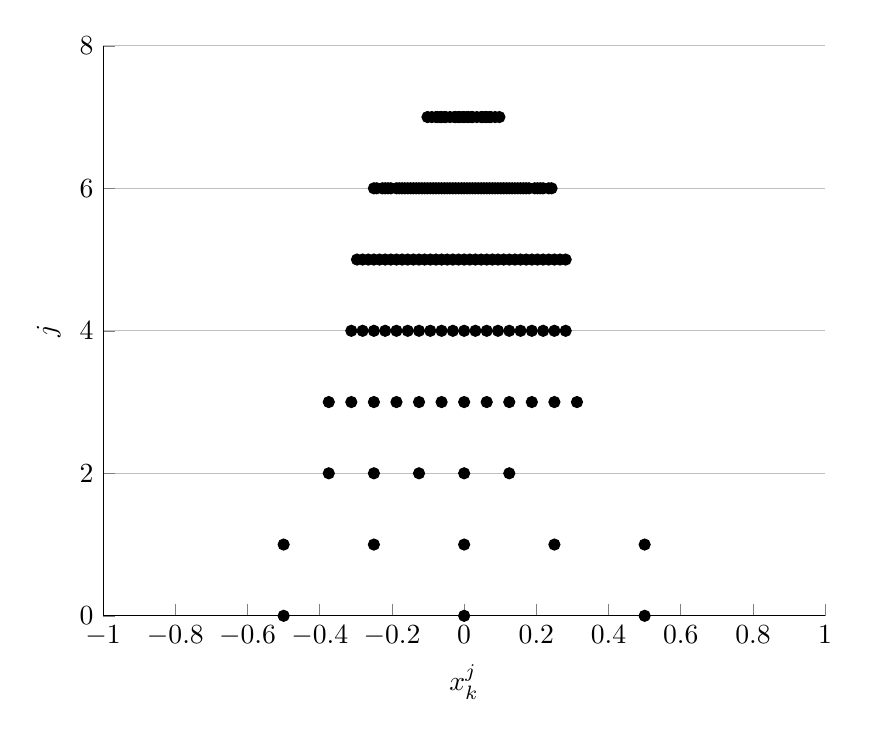
\begin{tikzpicture}

\begin{axis}[%
width=3.61in,
height=2.85in,
at={(1.01in,0.641in)},
scale only axis,
every outer x axis line/.append style={black},
every x tick label/.append style={font=\color{black}},
xmin=-1,
xmax=1,
xlabel={$x_{k}^{j}$},
every outer y axis line/.append style={black},
every y tick label/.append style={font=\color{black}},
ymin=0,
ymax=8,
ylabel={$j$},
ymajorgrids,
axis background/.style={fill=white},
axis x line*=bottom,
axis y line*=left
]
\addplot [color=black,only marks,mark=*,mark options={solid,fill=black,draw=black},forget plot]
  table[row sep=crcr]{%
-0.5	0\\
0	0\\
0.5	0\\
};
\addplot [color=black,only marks,mark=*,mark options={solid,fill=black,draw=black},forget plot]
  table[row sep=crcr]{%
-0.5	1\\
-0.25	1\\
0	1\\
0.25	1\\
0.5	1\\
};
\addplot [color=black,only marks,mark=*,mark options={solid,fill=black,draw=black},forget plot]
  table[row sep=crcr]{%
-0.5	-5\\
-0.375	2\\
-0.25	2\\
-0.125	2\\
0	2\\
0.125	2\\
0.25	-5\\
0.375	-5\\
0.5	-5\\
};
\addplot [color=black,only marks,mark=*,mark options={solid,fill=black,draw=black},forget plot]
  table[row sep=crcr]{%
-0.5	-5\\
-0.4375	-5\\
-0.375	3\\
-0.3125	3\\
-0.25	3\\
-0.1875	3\\
-0.125	3\\
-0.0625	3\\
0	3\\
0.0625	3\\
0.125	3\\
0.1875	3\\
0.25	3\\
0.3125	3\\
0.375	-5\\
0.4375	-5\\
0.5	-5\\
};
\addplot [color=black,only marks,mark=*,mark options={solid,fill=black,draw=black},forget plot]
  table[row sep=crcr]{%
-0.5	-5\\
-0.46875	-5\\
-0.4375	-5\\
-0.40625	-5\\
-0.375	-5\\
-0.34375	-5\\
-0.3125	4\\
-0.28125	4\\
-0.25	4\\
-0.21875	4\\
-0.1875	4\\
-0.15625	4\\
-0.125	4\\
-0.09375	4\\
-0.0625	4\\
-0.03125	4\\
0	4\\
0.03125	4\\
0.0625	4\\
0.09375	4\\
0.125	4\\
0.15625	4\\
0.1875	4\\
0.21875	4\\
0.25	4\\
0.28125	4\\
0.3125	-5\\
0.34375	-5\\
0.375	-5\\
0.40625	-5\\
0.4375	-5\\
0.46875	-5\\
0.5	-5\\
};
\addplot [color=black,only marks,mark=*,mark options={solid,fill=black,draw=black},forget plot]
  table[row sep=crcr]{%
-0.5	-5\\
-0.484375	-5\\
-0.46875	-5\\
-0.453125	-5\\
-0.4375	-5\\
-0.421875	-5\\
-0.40625	-5\\
-0.390625	-5\\
-0.375	-5\\
-0.359375	-5\\
-0.34375	-5\\
-0.328125	-5\\
-0.3125	-5\\
-0.296875	5\\
-0.28125	5\\
-0.265625	5\\
-0.25	5\\
-0.234375	5\\
-0.21875	5\\
-0.203125	5\\
-0.1875	5\\
-0.171875	5\\
-0.15625	5\\
-0.140625	5\\
-0.125	5\\
-0.109375	5\\
-0.09375	5\\
-0.078125	5\\
-0.0625	5\\
-0.046875	5\\
-0.03125	5\\
-0.015625	5\\
0	5\\
0.015625	5\\
0.03125	5\\
0.046875	5\\
0.0625	5\\
0.078125	5\\
0.09375	5\\
0.109375	5\\
0.125	5\\
0.140625	5\\
0.15625	5\\
0.171875	5\\
0.1875	5\\
0.203125	5\\
0.21875	5\\
0.234375	5\\
0.25	5\\
0.265625	5\\
0.28125	5\\
0.296875	-5\\
0.3125	-5\\
0.328125	-5\\
0.34375	-5\\
0.359375	-5\\
0.375	-5\\
0.390625	-5\\
0.40625	-5\\
0.421875	-5\\
0.4375	-5\\
0.453125	-5\\
0.46875	-5\\
0.484375	-5\\
0.5	-5\\
};
\addplot [color=black,only marks,mark=*,mark options={solid,fill=black,draw=black},forget plot]
  table[row sep=crcr]{%
-0.5	-5\\
-0.492188	-5\\
-0.484375	-5\\
-0.476562	-5\\
-0.46875	-5\\
-0.460938	-5\\
-0.453125	-5\\
-0.445312	-5\\
-0.4375	-5\\
-0.429688	-5\\
-0.421875	-5\\
-0.414062	-5\\
-0.40625	-5\\
-0.398438	-5\\
-0.390625	-5\\
-0.382812	-5\\
-0.375	-5\\
-0.367188	-5\\
-0.359375	-5\\
-0.351562	-5\\
-0.34375	-5\\
-0.335938	-5\\
-0.328125	-5\\
-0.320312	-5\\
-0.3125	-5\\
-0.304688	-5\\
-0.296875	-5\\
-0.289062	-5\\
-0.28125	-5\\
-0.273438	-5\\
-0.265625	-5\\
-0.257812	-5\\
-0.25	6\\
-0.242188	6\\
-0.234375	-5\\
-0.226562	6\\
-0.21875	6\\
-0.210938	6\\
-0.203125	6\\
-0.195312	-5\\
-0.1875	6\\
-0.179688	6\\
-0.171875	6\\
-0.164062	6\\
-0.15625	6\\
-0.148438	6\\
-0.140625	6\\
-0.132812	6\\
-0.125	6\\
-0.117188	6\\
-0.109375	6\\
-0.101562	6\\
-0.09375	6\\
-0.0859375	6\\
-0.078125	6\\
-0.0703125	6\\
-0.0625	6\\
-0.0546875	6\\
-0.046875	6\\
-0.0390625	6\\
-0.03125	6\\
-0.0234375	6\\
-0.015625	6\\
-0.0078125	6\\
0	6\\
0.0078125	6\\
0.015625	6\\
0.0234375	6\\
0.03125	6\\
0.0390625	6\\
0.046875	6\\
0.0546875	6\\
0.0625	6\\
0.0703125	6\\
0.078125	6\\
0.0859375	6\\
0.09375	6\\
0.101562	6\\
0.109375	6\\
0.117188	6\\
0.125	6\\
0.132812	6\\
0.140625	6\\
0.148438	6\\
0.15625	6\\
0.164062	6\\
0.171875	6\\
0.179688	6\\
0.1875	-5\\
0.195312	6\\
0.203125	6\\
0.210938	6\\
0.21875	6\\
0.226562	-5\\
0.234375	6\\
0.242188	6\\
0.25	-5\\
0.257812	-5\\
0.265625	-5\\
0.273438	-5\\
0.28125	-5\\
0.289062	-5\\
0.296875	-5\\
0.304688	-5\\
0.3125	-5\\
0.320312	-5\\
0.328125	-5\\
0.335938	-5\\
0.34375	-5\\
0.351562	-5\\
0.359375	-5\\
0.367188	-5\\
0.375	-5\\
0.382812	-5\\
0.390625	-5\\
0.398438	-5\\
0.40625	-5\\
0.414062	-5\\
0.421875	-5\\
0.429688	-5\\
0.4375	-5\\
0.445312	-5\\
0.453125	-5\\
0.460938	-5\\
0.46875	-5\\
0.476562	-5\\
0.484375	-5\\
0.492188	-5\\
0.5	-5\\
};
\addplot [color=black,only marks,mark=*,mark options={solid,fill=black,draw=black},forget plot]
  table[row sep=crcr]{%
-0.5	-5\\
-0.496094	-5\\
-0.492188	-5\\
-0.488281	-5\\
-0.484375	-5\\
-0.480469	-5\\
-0.476562	-5\\
-0.472656	-5\\
-0.46875	-5\\
-0.464844	-5\\
-0.460938	-5\\
-0.457031	-5\\
-0.453125	-5\\
-0.449219	-5\\
-0.445312	-5\\
-0.441406	-5\\
-0.4375	-5\\
-0.433594	-5\\
-0.429688	-5\\
-0.425781	-5\\
-0.421875	-5\\
-0.417969	-5\\
-0.414062	-5\\
-0.410156	-5\\
-0.40625	-5\\
-0.402344	-5\\
-0.398438	-5\\
-0.394531	-5\\
-0.390625	-5\\
-0.386719	-5\\
-0.382812	-5\\
-0.378906	-5\\
-0.375	-5\\
-0.371094	-5\\
-0.367188	-5\\
-0.363281	-5\\
-0.359375	-5\\
-0.355469	-5\\
-0.351562	-5\\
-0.347656	-5\\
-0.34375	-5\\
-0.339844	-5\\
-0.335938	-5\\
-0.332031	-5\\
-0.328125	-5\\
-0.324219	-5\\
-0.320312	-5\\
-0.316406	-5\\
-0.3125	-5\\
-0.308594	-5\\
-0.304688	-5\\
-0.300781	-5\\
-0.296875	-5\\
-0.292969	-5\\
-0.289062	-5\\
-0.285156	-5\\
-0.28125	-5\\
-0.277344	-5\\
-0.273438	-5\\
-0.269531	-5\\
-0.265625	-5\\
-0.261719	-5\\
-0.257812	-5\\
-0.253906	-5\\
-0.25	-5\\
-0.246094	-5\\
-0.242188	-5\\
-0.238281	-5\\
-0.234375	-5\\
-0.230469	-5\\
-0.226562	-5\\
-0.222656	-5\\
-0.21875	-5\\
-0.214844	-5\\
-0.210938	-5\\
-0.207031	-5\\
-0.203125	-5\\
-0.199219	-5\\
-0.195312	-5\\
-0.191406	-5\\
-0.1875	-5\\
-0.183594	-5\\
-0.179688	-5\\
-0.175781	-5\\
-0.171875	-5\\
-0.167969	-5\\
-0.164062	-5\\
-0.160156	-5\\
-0.15625	-5\\
-0.152344	-5\\
-0.148438	-5\\
-0.144531	-5\\
-0.140625	-5\\
-0.136719	-5\\
-0.132812	-5\\
-0.128906	-5\\
-0.125	-5\\
-0.121094	-5\\
-0.117188	-5\\
-0.113281	-5\\
-0.109375	-5\\
-0.105469	-5\\
-0.101562	7\\
-0.0976562	-5\\
-0.09375	-5\\
-0.0898438	7\\
-0.0859375	-5\\
-0.0820312	-5\\
-0.078125	7\\
-0.0742188	7\\
-0.0703125	-5\\
-0.0664062	7\\
-0.0625	7\\
-0.0585938	-5\\
-0.0546875	7\\
-0.0507812	7\\
-0.046875	-5\\
-0.0429688	-5\\
-0.0390625	7\\
-0.0351562	-5\\
-0.03125	-5\\
-0.0273438	7\\
-0.0234375	7\\
-0.0195312	-5\\
-0.015625	7\\
-0.0117188	7\\
-0.0078125	-5\\
-0.00390625	7\\
0	7\\
0.00390625	-5\\
0.0078125	7\\
0.0117188	7\\
0.015625	-5\\
0.0195312	7\\
0.0234375	7\\
0.0273438	-5\\
0.03125	-5\\
0.0351562	7\\
0.0390625	-5\\
0.0429688	-5\\
0.046875	7\\
0.0507812	7\\
0.0546875	-5\\
0.0585938	7\\
0.0625	7\\
0.0664062	-5\\
0.0703125	7\\
0.0742188	7\\
0.078125	-5\\
0.0820312	-5\\
0.0859375	7\\
0.0898438	-5\\
0.09375	-5\\
0.0976562	7\\
0.101562	-5\\
0.105469	-5\\
0.109375	-5\\
0.113281	-5\\
0.117188	-5\\
0.121094	-5\\
0.125	-5\\
0.128906	-5\\
0.132812	-5\\
0.136719	-5\\
0.140625	-5\\
0.144531	-5\\
0.148438	-5\\
0.152344	-5\\
0.15625	-5\\
0.160156	-5\\
0.164062	-5\\
0.167969	-5\\
0.171875	-5\\
0.175781	-5\\
0.179688	-5\\
0.183594	-5\\
0.1875	-5\\
0.191406	-5\\
0.195312	-5\\
0.199219	-5\\
0.203125	-5\\
0.207031	-5\\
0.210938	-5\\
0.214844	-5\\
0.21875	-5\\
0.222656	-5\\
0.226562	-5\\
0.230469	-5\\
0.234375	-5\\
0.238281	-5\\
0.242188	-5\\
0.246094	-5\\
0.25	-5\\
0.253906	-5\\
0.257812	-5\\
0.261719	-5\\
0.265625	-5\\
0.269531	-5\\
0.273438	-5\\
0.277344	-5\\
0.28125	-5\\
0.285156	-5\\
0.289062	-5\\
0.292969	-5\\
0.296875	-5\\
0.300781	-5\\
0.304688	-5\\
0.308594	-5\\
0.3125	-5\\
0.316406	-5\\
0.320312	-5\\
0.324219	-5\\
0.328125	-5\\
0.332031	-5\\
0.335938	-5\\
0.339844	-5\\
0.34375	-5\\
0.347656	-5\\
0.351562	-5\\
0.355469	-5\\
0.359375	-5\\
0.363281	-5\\
0.367188	-5\\
0.371094	-5\\
0.375	-5\\
0.378906	-5\\
0.382812	-5\\
0.386719	-5\\
0.390625	-5\\
0.394531	-5\\
0.398438	-5\\
0.402344	-5\\
0.40625	-5\\
0.410156	-5\\
0.414062	-5\\
0.417969	-5\\
0.421875	-5\\
0.425781	-5\\
0.429688	-5\\
0.433594	-5\\
0.4375	-5\\
0.441406	-5\\
0.445312	-5\\
0.449219	-5\\
0.453125	-5\\
0.457031	-5\\
0.460938	-5\\
0.464844	-5\\
0.46875	-5\\
0.472656	-5\\
0.476562	-5\\
0.480469	-5\\
0.484375	-5\\
0.488281	-5\\
0.492188	-5\\
0.496094	-5\\
0.5	-5\\
};
\addplot [color=black,only marks,mark=*,mark options={solid,fill=black,draw=black},forget plot]
  table[row sep=crcr]{%
-0.5	-5\\
-0.498047	-5\\
-0.496094	-5\\
-0.494141	-5\\
-0.492188	-5\\
-0.490234	-5\\
-0.488281	-5\\
-0.486328	-5\\
-0.484375	-5\\
-0.482422	-5\\
-0.480469	-5\\
-0.478516	-5\\
-0.476562	-5\\
-0.474609	-5\\
-0.472656	-5\\
-0.470703	-5\\
-0.46875	-5\\
-0.466797	-5\\
-0.464844	-5\\
-0.462891	-5\\
-0.460938	-5\\
-0.458984	-5\\
-0.457031	-5\\
-0.455078	-5\\
-0.453125	-5\\
-0.451172	-5\\
-0.449219	-5\\
-0.447266	-5\\
-0.445312	-5\\
-0.443359	-5\\
-0.441406	-5\\
-0.439453	-5\\
-0.4375	-5\\
-0.435547	-5\\
-0.433594	-5\\
-0.431641	-5\\
-0.429688	-5\\
-0.427734	-5\\
-0.425781	-5\\
-0.423828	-5\\
-0.421875	-5\\
-0.419922	-5\\
-0.417969	-5\\
-0.416016	-5\\
-0.414062	-5\\
-0.412109	-5\\
-0.410156	-5\\
-0.408203	-5\\
-0.40625	-5\\
-0.404297	-5\\
-0.402344	-5\\
-0.400391	-5\\
-0.398438	-5\\
-0.396484	-5\\
-0.394531	-5\\
-0.392578	-5\\
-0.390625	-5\\
-0.388672	-5\\
-0.386719	-5\\
-0.384766	-5\\
-0.382812	-5\\
-0.380859	-5\\
-0.378906	-5\\
-0.376953	-5\\
-0.375	-5\\
-0.373047	-5\\
-0.371094	-5\\
-0.369141	-5\\
-0.367188	-5\\
-0.365234	-5\\
-0.363281	-5\\
-0.361328	-5\\
-0.359375	-5\\
-0.357422	-5\\
-0.355469	-5\\
-0.353516	-5\\
-0.351562	-5\\
-0.349609	-5\\
-0.347656	-5\\
-0.345703	-5\\
-0.34375	-5\\
-0.341797	-5\\
-0.339844	-5\\
-0.337891	-5\\
-0.335938	-5\\
-0.333984	-5\\
-0.332031	-5\\
-0.330078	-5\\
-0.328125	-5\\
-0.326172	-5\\
-0.324219	-5\\
-0.322266	-5\\
-0.320312	-5\\
-0.318359	-5\\
-0.316406	-5\\
-0.314453	-5\\
-0.3125	-5\\
-0.310547	-5\\
-0.308594	-5\\
-0.306641	-5\\
-0.304688	-5\\
-0.302734	-5\\
-0.300781	-5\\
-0.298828	-5\\
-0.296875	-5\\
-0.294922	-5\\
-0.292969	-5\\
-0.291016	-5\\
-0.289062	-5\\
-0.287109	-5\\
-0.285156	-5\\
-0.283203	-5\\
-0.28125	-5\\
-0.279297	-5\\
-0.277344	-5\\
-0.275391	-5\\
-0.273438	-5\\
-0.271484	-5\\
-0.269531	-5\\
-0.267578	-5\\
-0.265625	-5\\
-0.263672	-5\\
-0.261719	-5\\
-0.259766	-5\\
-0.257812	-5\\
-0.255859	-5\\
-0.253906	-5\\
-0.251953	-5\\
-0.25	-5\\
-0.248047	-5\\
-0.246094	-5\\
-0.244141	-5\\
-0.242188	-5\\
-0.240234	-5\\
-0.238281	-5\\
-0.236328	-5\\
-0.234375	-5\\
-0.232422	-5\\
-0.230469	-5\\
-0.228516	-5\\
-0.226562	-5\\
-0.224609	-5\\
-0.222656	-5\\
-0.220703	-5\\
-0.21875	-5\\
-0.216797	-5\\
-0.214844	-5\\
-0.212891	-5\\
-0.210938	-5\\
-0.208984	-5\\
-0.207031	-5\\
-0.205078	-5\\
-0.203125	-5\\
-0.201172	-5\\
-0.199219	-5\\
-0.197266	-5\\
-0.195312	-5\\
-0.193359	-5\\
-0.191406	-5\\
-0.189453	-5\\
-0.1875	-5\\
-0.185547	-5\\
-0.183594	-5\\
-0.181641	-5\\
-0.179688	-5\\
-0.177734	-5\\
-0.175781	-5\\
-0.173828	-5\\
-0.171875	-5\\
-0.169922	-5\\
-0.167969	-5\\
-0.166016	-5\\
-0.164062	-5\\
-0.162109	-5\\
-0.160156	-5\\
-0.158203	-5\\
-0.15625	-5\\
-0.154297	-5\\
-0.152344	-5\\
-0.150391	-5\\
-0.148438	-5\\
-0.146484	-5\\
-0.144531	-5\\
-0.142578	-5\\
-0.140625	-5\\
-0.138672	-5\\
-0.136719	-5\\
-0.134766	-5\\
-0.132812	-5\\
-0.130859	-5\\
-0.128906	-5\\
-0.126953	-5\\
-0.125	-5\\
-0.123047	-5\\
-0.121094	-5\\
-0.119141	-5\\
-0.117188	-5\\
-0.115234	-5\\
-0.113281	-5\\
-0.111328	-5\\
-0.109375	-5\\
-0.107422	-5\\
-0.105469	-5\\
-0.103516	-5\\
-0.101562	-5\\
-0.0996094	-5\\
-0.0976562	-5\\
-0.0957031	-5\\
-0.09375	-5\\
-0.0917969	-5\\
-0.0898438	-5\\
-0.0878906	-5\\
-0.0859375	-5\\
-0.0839844	-5\\
-0.0820312	-5\\
-0.0800781	-5\\
-0.078125	-5\\
-0.0761719	-5\\
-0.0742188	-5\\
-0.0722656	-5\\
-0.0703125	-5\\
-0.0683594	-5\\
-0.0664062	-5\\
-0.0644531	-5\\
-0.0625	-5\\
-0.0605469	-5\\
-0.0585938	-5\\
-0.0566406	-5\\
-0.0546875	-5\\
-0.0527344	-5\\
-0.0507812	-5\\
-0.0488281	-5\\
-0.046875	-5\\
-0.0449219	-5\\
-0.0429688	-5\\
-0.0410156	-5\\
-0.0390625	-5\\
-0.0371094	-5\\
-0.0351562	-5\\
-0.0332031	-5\\
-0.03125	-5\\
-0.0292969	-5\\
-0.0273438	-5\\
-0.0253906	-5\\
-0.0234375	-5\\
-0.0214844	-5\\
-0.0195312	-5\\
-0.0175781	-5\\
-0.015625	-5\\
-0.0136719	-5\\
-0.0117188	-5\\
-0.00976562	-5\\
-0.0078125	-5\\
-0.00585938	-5\\
-0.00390625	-5\\
-0.00195312	-5\\
0	-5\\
0.00195312	-5\\
0.00390625	-5\\
0.00585938	-5\\
0.0078125	-5\\
0.00976562	-5\\
0.0117188	-5\\
0.0136719	-5\\
0.015625	-5\\
0.0175781	-5\\
0.0195312	-5\\
0.0214844	-5\\
0.0234375	-5\\
0.0253906	-5\\
0.0273438	-5\\
0.0292969	-5\\
0.03125	-5\\
0.0332031	-5\\
0.0351562	-5\\
0.0371094	-5\\
0.0390625	-5\\
0.0410156	-5\\
0.0429688	-5\\
0.0449219	-5\\
0.046875	-5\\
0.0488281	-5\\
0.0507812	-5\\
0.0527344	-5\\
0.0546875	-5\\
0.0566406	-5\\
0.0585938	-5\\
0.0605469	-5\\
0.0625	-5\\
0.0644531	-5\\
0.0664062	-5\\
0.0683594	-5\\
0.0703125	-5\\
0.0722656	-5\\
0.0742188	-5\\
0.0761719	-5\\
0.078125	-5\\
0.0800781	-5\\
0.0820312	-5\\
0.0839844	-5\\
0.0859375	-5\\
0.0878906	-5\\
0.0898438	-5\\
0.0917969	-5\\
0.09375	-5\\
0.0957031	-5\\
0.0976562	-5\\
0.0996094	-5\\
0.101562	-5\\
0.103516	-5\\
0.105469	-5\\
0.107422	-5\\
0.109375	-5\\
0.111328	-5\\
0.113281	-5\\
0.115234	-5\\
0.117188	-5\\
0.119141	-5\\
0.121094	-5\\
0.123047	-5\\
0.125	-5\\
0.126953	-5\\
0.128906	-5\\
0.130859	-5\\
0.132812	-5\\
0.134766	-5\\
0.136719	-5\\
0.138672	-5\\
0.140625	-5\\
0.142578	-5\\
0.144531	-5\\
0.146484	-5\\
0.148438	-5\\
0.150391	-5\\
0.152344	-5\\
0.154297	-5\\
0.15625	-5\\
0.158203	-5\\
0.160156	-5\\
0.162109	-5\\
0.164062	-5\\
0.166016	-5\\
0.167969	-5\\
0.169922	-5\\
0.171875	-5\\
0.173828	-5\\
0.175781	-5\\
0.177734	-5\\
0.179688	-5\\
0.181641	-5\\
0.183594	-5\\
0.185547	-5\\
0.1875	-5\\
0.189453	-5\\
0.191406	-5\\
0.193359	-5\\
0.195312	-5\\
0.197266	-5\\
0.199219	-5\\
0.201172	-5\\
0.203125	-5\\
0.205078	-5\\
0.207031	-5\\
0.208984	-5\\
0.210938	-5\\
0.212891	-5\\
0.214844	-5\\
0.216797	-5\\
0.21875	-5\\
0.220703	-5\\
0.222656	-5\\
0.224609	-5\\
0.226562	-5\\
0.228516	-5\\
0.230469	-5\\
0.232422	-5\\
0.234375	-5\\
0.236328	-5\\
0.238281	-5\\
0.240234	-5\\
0.242188	-5\\
0.244141	-5\\
0.246094	-5\\
0.248047	-5\\
0.25	-5\\
0.251953	-5\\
0.253906	-5\\
0.255859	-5\\
0.257812	-5\\
0.259766	-5\\
0.261719	-5\\
0.263672	-5\\
0.265625	-5\\
0.267578	-5\\
0.269531	-5\\
0.271484	-5\\
0.273438	-5\\
0.275391	-5\\
0.277344	-5\\
0.279297	-5\\
0.28125	-5\\
0.283203	-5\\
0.285156	-5\\
0.287109	-5\\
0.289062	-5\\
0.291016	-5\\
0.292969	-5\\
0.294922	-5\\
0.296875	-5\\
0.298828	-5\\
0.300781	-5\\
0.302734	-5\\
0.304688	-5\\
0.306641	-5\\
0.308594	-5\\
0.310547	-5\\
0.3125	-5\\
0.314453	-5\\
0.316406	-5\\
0.318359	-5\\
0.320312	-5\\
0.322266	-5\\
0.324219	-5\\
0.326172	-5\\
0.328125	-5\\
0.330078	-5\\
0.332031	-5\\
0.333984	-5\\
0.335938	-5\\
0.337891	-5\\
0.339844	-5\\
0.341797	-5\\
0.34375	-5\\
0.345703	-5\\
0.347656	-5\\
0.349609	-5\\
0.351562	-5\\
0.353516	-5\\
0.355469	-5\\
0.357422	-5\\
0.359375	-5\\
0.361328	-5\\
0.363281	-5\\
0.365234	-5\\
0.367188	-5\\
0.369141	-5\\
0.371094	-5\\
0.373047	-5\\
0.375	-5\\
0.376953	-5\\
0.378906	-5\\
0.380859	-5\\
0.382812	-5\\
0.384766	-5\\
0.386719	-5\\
0.388672	-5\\
0.390625	-5\\
0.392578	-5\\
0.394531	-5\\
0.396484	-5\\
0.398438	-5\\
0.400391	-5\\
0.402344	-5\\
0.404297	-5\\
0.40625	-5\\
0.408203	-5\\
0.410156	-5\\
0.412109	-5\\
0.414062	-5\\
0.416016	-5\\
0.417969	-5\\
0.419922	-5\\
0.421875	-5\\
0.423828	-5\\
0.425781	-5\\
0.427734	-5\\
0.429688	-5\\
0.431641	-5\\
0.433594	-5\\
0.435547	-5\\
0.4375	-5\\
0.439453	-5\\
0.441406	-5\\
0.443359	-5\\
0.445312	-5\\
0.447266	-5\\
0.449219	-5\\
0.451172	-5\\
0.453125	-5\\
0.455078	-5\\
0.457031	-5\\
0.458984	-5\\
0.460938	-5\\
0.462891	-5\\
0.464844	-5\\
0.466797	-5\\
0.46875	-5\\
0.470703	-5\\
0.472656	-5\\
0.474609	-5\\
0.476562	-5\\
0.478516	-5\\
0.480469	-5\\
0.482422	-5\\
0.484375	-5\\
0.486328	-5\\
0.488281	-5\\
0.490234	-5\\
0.492188	-5\\
0.494141	-5\\
0.496094	-5\\
0.498047	-5\\
0.5	-5\\
};
\end{axis}
\end{tikzpicture}%
	\caption{Coefficients kept with $\epsilon=10^{-3}$.}
\end{figure}
\newpage
\section{To Be Completed Soon}
\begin{enumerate}
	\item Implement code for calculating spatial derivatives. When a particular point on $\mathcal{G}^{j+1}$ is absent 
		of its detail coefficient (due to the threshold, or $j+1$ is the maximum level of refinement), then the approximation 
		from the interpolating polynomial constructed on $\mathcal{G}^j$ is good enough. Thus differentiating the local
		polynomial is a good enough approximation to the derivative of the function at that location.
	\item The issue of the detail coefficient at the last point in the grid must be solved. As can be seen in Figure 5 and 
		Figure 7, the detail coefficients are not being calculated correctly at the very last index. This would depend on 
		interpolating at a ghost point possibly, so I am determining the best way to deal with the issue.
	\item The additional 'lifting' step requires adjustment of 3 lines of code in the program. One simply also constructs
		interpolating polynomials from the odd points to the even points. I wanted to get the code working properly before 
		moving on to this necessary step. 
\end{enumerate}

\end{document}
